\documentclass[12pt,a4paper,%
%draft%
]{scrreprt}
% prevent warning \float@addtolists detected
\usepackage{scrhack} 

% Textkodierung Deutsch
\usepackage[ngerman]{babel}
\usepackage[T1]{fontenc}
\usepackage[utf8]{inputenc}
\usepackage{lmodern}
\usepackage{xspace}
\usepackage{microtype}

% Basisinfos
\title{Modellbasierte Testautomatisierung eines verteilen, adaptiven Load-Balancing-Systems}
\author{Gerald Siegert}
\date{\today}
%Variablen welche innerhalb der gesamten Arbeit zur Verfügung stehen sollen
\newcommand{\titleDocument}{Masterarbeit}
\newcommand{\subjectDocument}{im Studiengang Informatik}
\newcommand{\zB}{z.\,B. }
\newcommand{\uA}{u.\,A. }
\newcommand{\sS}{S\# }
\newcommand{\cS}{C\# }
\newcommand{\uU}{unter Umständen}
%hier müssen alle Wörter rein, welche Latex von sich auch nicht korrekt trennt bzw. bei denen man die genaue Trennung vorgeben möchte
\hyphenation
{
    Film-pro-du-zen-ten
    Lux-em-burg
    Soft-ware-bau-steins
    zeit-in-ten-siv
}
\renewcommand{\texttt}[1]{%
    \begingroup
    \ttfamily
    \begingroup\lccode`~=`/\lowercase{\endgroup\def~}{/\discretionary{}{}{}}%
    \begingroup\lccode`~=`[\lowercase{\endgroup\def~}{[\discretionary{}{}{}}%
    \begingroup\lccode`~=`.\lowercase{\endgroup\def~}{.\discretionary{}{}{}}%
    \catcode`/=\active\catcode`[=\active\catcode`.=\active
    \scantokens{#1\noexpand}%
    \endgroup
}

% Seitenränder
\usepackage{geometry}
\geometry{left=35mm,right=20mm,top=25mm,bottom=20mm}

% Kopf/Fußzeilen
\usepackage[headsepline]{scrlayer-scrpage}
\clearscrheadfoot
\pagestyle{scrheadings}

\ihead{\headmark}
\automark{chapter}
\ohead{\pagemark}

\renewcommand*{\headfont}{\normalfont}
\setlength{\headheight}{1.5\baselineskip}
\renewcommand*{\chapterpagestyle}{scrheadings}

\newpairofpagestyles[scrheadings]{lists}{%
    \ihead{Verzeichnisse}%
}

% Grafiken
\usepackage{graphicx}
\usepackage{wrapfig}
\usepackage[format=plain]{caption}
\setkeys{Gin}{width=0.8\columnwidth} % default width
 
% Tabellen
\usepackage{multirow}
\usepackage{tabu}

% Textfarben
\usepackage{xcolor}

% Abkürzungen
\usepackage[nohyperlinks,printonlyused]{acronym}

% Zeilenabstand
\usepackage[onehalfspacing]{setspace}
\usepackage{enumitem}
% noitemsep bei listen
\setlist[itemize]{noitemsep}
\setlist[enumerate]{noitemsep}
% Abstand vor Kapiteltitel
\renewcommand*{\chapterheadstartvskip}{\vspace*{.5\baselineskip}}

% Literatur
\usepackage[style=numeric-comp,%
    natbib=true,%
    maxitems=1,%
    backend=biber,%
    sorting=none]{biblatex}
\usepackage{csquotes}
\addbibresource{./literatur/literatur.bib}
\addbibresource{./literatur/web.bib}
\addbibresource{./literatur/abbildungen.bib}
% Zeilenumbrüche bei URLs
\setcounter{biburllcpenalty}{7000}
\setcounter{biburlucpenalty}{8000}

% Listings
\usepackage{listings}
\makeatletter
\definecolor{bluekeywords}{rgb}{0.13,0.13,1}
\definecolor{greencomments}{rgb}{0,0.5,0}
\definecolor{redstrings}{rgb}{0.9,0,0}
\definecolor{typeidentifier}{RGB}{38,121,153}
\definecolor{backgroundgray}{rgb}{0.95,0.95,0.95}
\lstdefinestyle{base}{
    basicstyle=\footnotesize\ttfamily,
    frame=single,
    backgroundcolor=\color{backgroundgray},
    numbers=left,
    numberstyle=\tiny,
    numbersep=7pt,
    breaklines=true,
    tabsize=2,
    captionpos=b,
    extendedchars=true,
    showstringspaces=false,
}
\lstdefinestyle{cs}{
    language=[sharp]c,
    style=base,
    morekeywords={get,set,var,nameof,yield},
    keywordstyle=\color{bluekeywords}\bfseries,
    commentstyle=\color{greencomments},
    stringstyle=\color{redstrings},
}
\lstdefinestyle{plain}{
    language={},
    style=base,
    tabsize=4,
    captionpos=t,
}
% Json Listings
\newcommand\JSONnumbervaluestyle{\color{blue}}
\newcommand\JSONstringvaluestyle{\color{red}}
% switch used as state variable
\newif\ifcolonfoundonthisline
\lstdefinestyle{json}
{
    style=base,
    captionpos=t,
    showstringspaces    = false,
    keywords            = {false,true},
    alsoletter          = 0123456789.,
    morestring          = [s]{"}{"},
    stringstyle         = \ifcolonfoundonthisline\JSONstringvaluestyle\fi,
    MoreSelectCharTable =%
    \lst@DefSaveDef{`:}\colon@json{\processColon@json},
    keywordstyle        = \bfseries,
}
% flip the switch if a colon is found in Pmode
\newcommand\processColon@json{%
    \colon@json%
    \ifnum\lst@mode=\lst@Pmode%
    \global\colonfoundonthislinetrue%
    \fi
}
\lst@AddToHook{Output}{%
    \ifcolonfoundonthisline%
    \ifnum\lst@mode=\lst@Pmode%
    \def\lst@thestyle{\JSONnumbervaluestyle}%
    \fi
    \fi
    %override by keyword style if a keyword is detected!
    \lsthk@DetectKeywords% 
}
% reset the switch at the end of line
\lst@AddToHook{EOL}%
{\global\colonfoundonthislinefalse}
%%%%%%%%%% end listings

\makeatletter

% Default centering floatboxes
\g@addto@macro\@floatboxreset\centering

% Verzeichnisse
\renewcommand\listoffigures{%
    \addsec{\listfigurename}%
    \@mkboth{\MakeUppercase\listfigurename}%
    {\listfigurename}%
    \@starttoc{lof}%
}
\renewcommand\listoftables{%
    \addsec{\listtablename}%
    \@mkboth{\MakeUppercase\listtablename}%
    {\listtablename}%
    \@starttoc{lot}%
}
\renewcommand\lstlistoflistings{%
    \addsec{\lstlistlistingname}%
    \@mkboth{\MakeUppercase\lstlistlistingname}%
    {\lstlistlistingname}%
    \@starttoc{lol}%
}

\makeatother

% Hurenkinder, Schusterjungen
\clubpenalty = 10000
\widowpenalty = 10000
\displaywidowpenalty = 10000 

% Referenzen
\PassOptionsToPackage{hyphens}{url}\usepackage{hyperref}

\usepackage{todonotes}
\presetkeys{todonotes}{inline}{}

\begin{document}
    % Titelseite
    \setcounter{page}{-100}
    \begin{titlepage}
        \begin{doublespace}
            \begin{center}
    {\Large{Universität Augsburg\\Fakultät für Angewandte Informatik}}
    \vspace{4\baselineskip}
    
    \begin{onehalfspace}
        \textbf{\large{Modellbasierte Testautomatisierung eines\\verteilten, adaptiven Load-Balancing-Systems}}
    \end{onehalfspace}
    \vspace{3\baselineskip}
    
    \textbf{{\Large{Masterarbeit}}}
    \vspace{1\baselineskip}
    
    \textbf{im Studiengang Informatik}
    \vspace{1\baselineskip}
    
    \textbf{zur Erlangung des akademischen Grades\\Master of Science}
    \vspace{1\baselineskip}
    
    \textbf{von\\Gerald Siegert}
    \vspace{\fill}
    
    \begin{singlespace}
        \begin{tabular}{llll}
            \textbf{Mat.-Nr.:}  &  & 1450117                      &  \\
            &  &  \\
            \textbf{Datum:}     &  & \today                       &  \\
            &  &  \\
            \textbf{Betreuer:}  &  & M.Sc. Benedikt Eberhardinger &  \\
            \textbf{1. Prüfer:} &  & Prof. Dr. X                  &  \\
            \textbf{2. Prüfer:} &  & Prof. Dr. Y                  &
        \end{tabular}
    \end{singlespace}
\end{center}

        \end{doublespace}
    \end{titlepage}
    
    % Abstract
    \pagenumbering{Roman}
    \begin{abstract}
    Durch eine Automatisierung von Tests lassen sich im Bereich der Softwareentwicklung hohe Kosten einsparen.
    Daher wurden zahlreiche Test"=Frameworks und Möglichkeiten zum Testen von Systemen und ihrer Software entwickelt.
    Ein solches Framework ist \acrshort{ss} (\acrlong{ss}), mit dem mithilfe eines modellbasierten Ansatzes Systeme getestet werden können.
    Mithilfe des \acrshort{ss}"=Frameworks soll nun ein Testsystem entwickelt werden, um hiermit automatisiert ein verteiltes, adaptives Load"=Balancing"=System zu testen.
    Hierfür wurde Apache Hadoop ausgewählt, welches mit einer selbstadaptiven Komponente ergänzt wird.
    Diese selbstadaptive Komponente verändert dynamisch und basierend auf den derzeit auf dem Hadoop"=Cluster ausgeführten Anwendungen einige der sonst statischen Einstellungen von Hadoop, womit die verfügbaren Ressourcen des Clusters optimaler genutzt werden können.
    
    Um Hadoop testen zu können, wurde zunächst mithilfe von \acrshort{ss} ein Modell entwickelt, welches die wesentlichen Komponenten des YARN=Frameworks von Hadoop abbildet.
    Dieses Modell wurde wiederum mithilfe eines hierfür entwickelten Treibers mit einem realen Hadoop"=Cluster verbunden.
    Dadurch wurde es ermöglicht, durch die Testausführung mit \acrshort{ss} unterschiedliche Anwendungen auf dem realen Cluster auszuführen und die Daten der Anwendungen und des Clusters im Modell zu nutzen.
    Um zu testen, ob sich das entwickelte Testsystem zur Testautomatisierung eines verteilten, adaptiven Load"=Balancing"=Systems eignet, wurde hierfür eine Fallstudie durchgeführt.
    
    In dieser Masterarbeit werden der Aufbau und Ablauf der durchgeführten Fallstudie, sowie die Entwicklung und Implementierung des hierfür genutzten Testsystems erläutert.
    Es wird gezeigt, welche Besonderheiten bei der Durchführung und Auswertung der Fallstudie aufgetreten sind, und inwiefern sich das entwickelte, modellbasierte Testsystem zur Testautomatisierung eines verteilten, adaptiven Load"=Balancing"=Systems eignet.
\end{abstract}

\clearpage
\begin{otherlanguage}{english}
\begin{abstract}
    By automating tests, high costs can be saved in software development.
    Therefore, numerous test frameworks and ways to test systems and their software have been developed.
    One such framework is \acrshort{ss} (\acrlong{ss}), which uses a model-based approach to test systems.
    By using the \acrshort{ss} framework, a test system will be developed to automatically test a distributed, adaptive load-balancing system.
    For this, Apache Hadoop was chosen, which is equipped with an adaptive resource manager.
    The manager detect the current usage of the cluster and modify some of Hadoop's otherwise static settings to make a better use of the available resources.
    
    To test hadoop, a \acrshort{ss} model was developed, which contains the essential componentens of the Hadoop YARN framework.
    To connect the model to a real Hadoop cluster a driver was developed for this purpose.
    This allows \acrshort{ss} to run different applications on the real cluster and detect the state of the running applications and the cluster.
    To determine the developed test system is suitable for the test automation of a distributed, adaptive load-balancing system, a case study was performed.
    
    This master thesis explains the structure and processes of the case study, as well as the development and implementation of the test system used for this purpose.
    It shows the won experiences by performing the case study and shows how the developed, model-based test system is suitable for test automation of a distributed, adaptive load-balancing system.
\end{abstract}
\end{otherlanguage}


    
    % Verzeichnisse
    \newpage
    \begin{singlespace}
        \tableofcontents
        %\addchap{Verzeichnisse}

\addcontentsline{toc}{chapter}{Literatur}
%\renewcommand\refname{Literatur}
\printbibliography

\addcontentsline{toc}{chapter}{Abbildungsverzeichnis}
%\renewcommand{\listfigurename}{Abbildungen}
\listoffigures

\addcontentsline{toc}{chapter}{Listings}
%\renewcommand{\lstlistlistingname}{Listings}
\lstlistoflistings

\addcontentsline{toc}{chapter}{Tabellenverzeichnis}
%\renewcommand{\listtablename}{Tabellen}
\listoftables

\addcontentsline{toc}{chapter}{Verzeichnis der Algorithmen}
%\renewcommand{\listalgorithmname}{Algorithmen}
\listofalgorithms

    \end{singlespace}
    
    % Inhalt
    \pagestyle{scrheadings}
    \newpage
    \pagenumbering{arabic}
    
    \chapter{Einleitung}
\label{chap:intro}

Im Bereich der Softwaretests wird heutzutage sehr viel mit automatisierten Testverfahren gearbeitet.
Dies ist insofern logisch, als dass diese Testautomatisierung einerseits Aufwand und damit andererseits direkt Kosten einer Software einspart.
Daher gibt es vor allem im Bereich der Komponententests zahlreiche Frameworks, mit denen Tests einfach und automatisiert erstellt bzw. ausgeführt werden können.
Ein Beispiel für ein solches Testframework wäre das \emph{xUnit}"=Framework, zu dem \uA JUnit\footnote{\url{https://junit.org}} für Java und NUnit\footnote{\url{https://nunit.org/}} für .NET zählen.
Dabei werden zunächst einzelne Testfälle erstellt und können im Anschluss mit der jeweils aktuellen Codebasis jederzeit ausgeführt werden.
Automatisierte Tests können auch dazu genutzt werden, um einen einzelnen Test mit verschiedenen Eingaben durchzuführen.
Dadurch können verschiedene Eingabeklassen (wie negative oder positive Ganzzahlen) mit sehr geringem Aufwand in einem Test genutzt werden und somit verschiedene Testfälle direkt ausgeführt werden, wodurch eine massive Kosteneinsparung einhergeht \cite{Polo2013}.

Es gibt aber nicht nur Frameworks für Komponententests, sondern auch für modellbasierte Testverfahren wie \zB dem \ac{MC}.
Beim \ac{MC} wird ein Modell mithilfe eines entsprechenden Frameworks automatisiert auf seine Spezifikation getestet und geprüft, unter welchen Umständen diese verletzt wird \cite{Grumberg1999,Habermaier2015}.

In dieser Masterarbeit soll daher nun ein verteiltes, adaptives Load"=Balancing"=System getestet werden.
Hauptziel ist es, zu ermitteln, wie ein modellbasierter Testansatz auf ein komplexes Beispiel übertragen werden kann.
Dafür wird zunächst ein reales System als vereinfachtes Modell nachgebildet und anschließend mithilfe eines \ac{MC} getestet.
Es soll dabei auch ermittelt werden, wie ein reales System in das Modell eingebunden werden kann und wie bei Problemen mit asynchronen Prozessen innerhalb des verteilten Systems umgegangen werden muss.

    \chapter{Grundlagen und Stand der Technik}
\label{ch:basics}

\todo{Einleitungstext}

%\section{Model Checking}\label{sec:modelchecking}

\ac{MC} ist eine Möglichkeit, um Systeme zu testen und zu verifizieren. Dazu werden vom \ac{MCr} alle möglichen Systemzustände in einem \emph{brute-force}-ähnlichem Vorgehen getestet und somit alle möglichen Szenarien getestet. Die Anzahl der Zustände kann sehr schnell $ 10^{120} $ oder mehr betragen \cite{Grumberg1999,Baier2008}.

\begin{figure}
	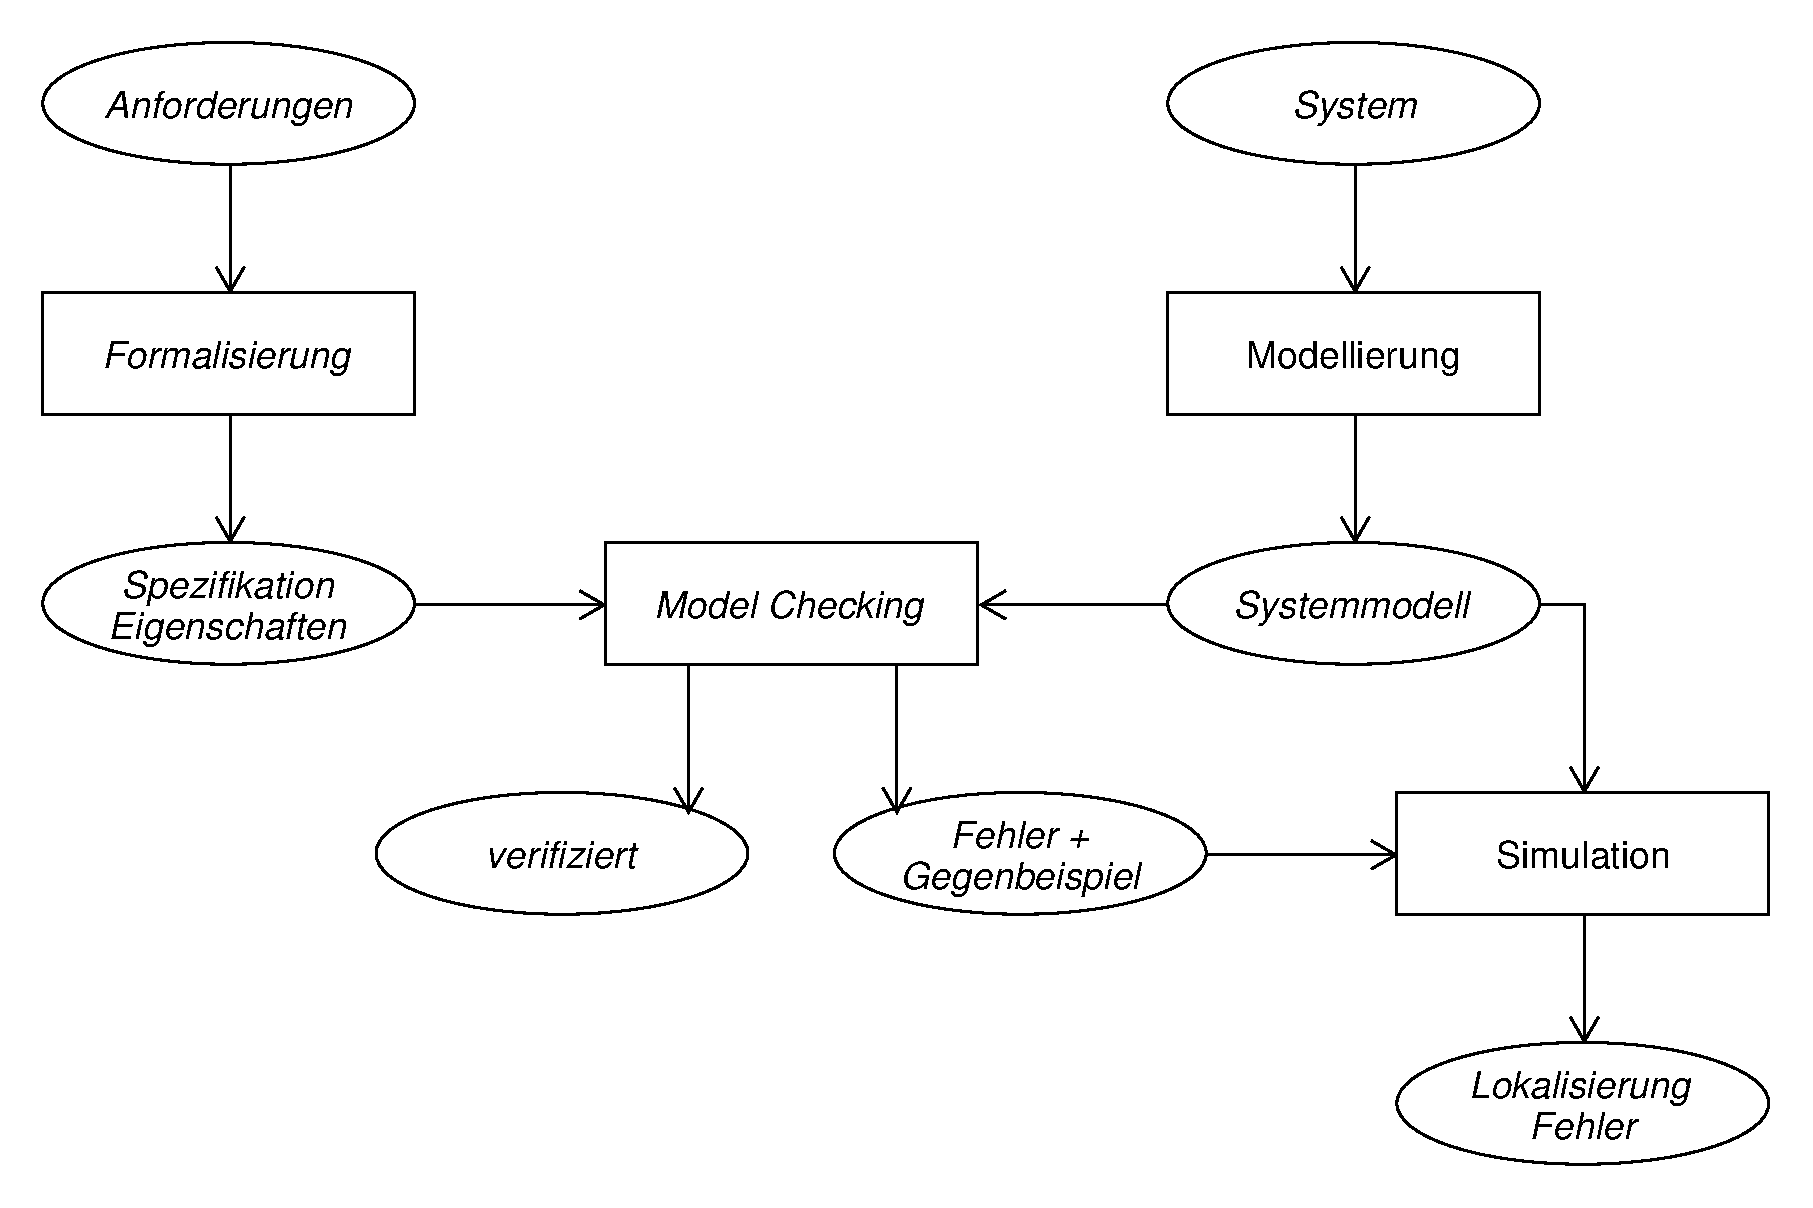
\includegraphics{./images/mcSchema.pdf}
	\caption[Schematischer Aufbau beim MC]{Schematischer Aufbau beim MC, nach \cite{Baier2008}}
	\label{fig:mcSchema}
\end{figure}

Ein \ac{MCr} nutzt, wie der Name schon sagt, ein Modell des Systems, um das System zu testen. Wie bei jeder anderen modellbasierten Technik ist daher die Qualität des \ac{MC} nur so gut wie das darauf zugrunde liegende Modell. Ein Modell kann auch als endlicher Automat angesehen werden, da ein Modell ebenfalls eine endliche Anzahl an möglichen Zuständen und dazugehörige Übergänge besitzt. Für jede Eigenschaft eines Zustandes muss zudem mithilfe einer sog. \emph{temporalen Logik}, also mathematisch bzw. formal, festgelegt werden, was gültige Werte dieser Eigenschaft sind. Die dazu benötigten Informationen werden aus den Anforderungen des Systems ermittelt und dem \ac{MCr} übergeben. So können später verschiedene Eigenschaften des gesamten Systems (\zB die formale Korrektheit, die Ausführbarkeit ohne Deadlocks oder die Einhaltung von Sicherheitsvorgaben) geprüft werden.

Zur Ausführung wird das gesamte Modell zunächst initialisiert und dann automatisch und systematisch vom \ac{MCr} auf Fehler und ungültige Zustände geprüft. In der Regel ist aber auch eine Ausführung als reine Simulation des Systems möglich, ohne explizit nach Fehlern zu suchen.

Wenn alle Zustände und deren Eigenschaften die Anforderungen erfüllen, erfüllt auch das Modell die Spezifikation. Wenn ein Zustand bzw. Eigenschaft die Anforderungen nicht erfüllt, prüft der \ac{MCr} anhand eines Gegenbeispiels den Ausführungspfad zum Fehler. Dadurch kann ermittelt werden, wo die Fehlerursache liegt. Einige der wesentlichen Fehlertypen und Ursachen sind:

\begin{description}
	\item[Modelling Error] Der Fehler liegt im Modell, welches korrigiert werden muss.
	\item[Design Error] Der Fehler liegt in den formellen oder informellen Anforderungen, dadurch muss das Modell und/oder die temporale Logik korrigiert werden.
	\item[Property Error] Der Fehler ist wirklich ein Fehler im System, welcher gefunden werden soll.
\end{description}

Möglich ist aber auch, dass die Ressourcen nicht ausreichen, um alle Zustände zu prüfen. In so einem Fall gibt es mehrere Möglichkeiten, damit umzugehen, \zB können Heuristiken oder Abstraktionen vom Modell genutzt werden \cite{Baier2008,Eberhardinger2016}.

\ac{MC} besitzt durch seine Charakteristik einige Vorteile, \uA \cite{Baier2008}:
\begin{itemize}
	\item \ac{MC} ist universell nutzbar, \zB für Software, Hardware oder eingebettete Systeme
	\item Partielle Verifikation ist möglich ohne das gesamte System testen zu müssen
	\item Vollständig automatisierbar und benötigt kaum Benutzerinteraktion oder hohe Expertise
\end{itemize}

Natürlich gibt es aber auch einige Nachteile, \uA \cite{Baier2008}:
\begin{itemize}
	\item Mit \ac{MC} wird nur ein Systemmodell und nicht das eigentliche System getestet, was weitere Fehler nicht ausschließt
	\item Hauptsächlich für steuerungsbasierte Anwendungen und nicht für datenbasierte Anwendungen geeignet
	\item Anzahl der möglichen Zustände kann zu hoch sein, um alle zu testen
\end{itemize}

Es gibt zahlreiche \ac{MC}-Frameworks, die bereits erwähnten \emph{LTSmin} und \emph{\sS} sind nur zwei davon.

\section{\acl{ss}}
\label{sec:ssharp}

\todo{Testen unter SS allgemein genauer erklären}
\textbf{\acf{ss}} ist ein am \isse der Universität Augsburg entwickeltes Framework zum Testen und Verifizieren von Systemen und Modellen.
Da es in \cS entwickelt wurde und \cS auch zum Entwickeln von Modellen und dazugehörigen Testszenarien genutzt wird, können zahlreiche Features des .NET"=Frameworks bzw. der Sprache \cS im Speziellen genutzt werden.
\ac{ss} vereint dabei die Simulation, die Visualisierung, modellbasierte Tests sowie die Verifizierung der Modelle durch einen \ac{MCr} \cite{Habermaier2015,Habermaier2016}.
Dadurch können alle Schritte einer vollständigen Analyse inkl. Modellierung direkt im Visual Studio ausgeführt werden und somit auch alle Features der IDE und .NET, wie \zB die Debugging"=Werkzeuge, genutzt werden.
Um entsprechende Analysen zu gewährleisten, hat das Framework jedoch auch einige Einschränkungen, wodurch \zB Schleifen und Rekursionen nur eingeschränkt bzw. nicht möglich sind.
Eine der größten Einschränkungen ist allerdings, dass während der Laufzeit keine neuen Objektinstanzen innerhalb des zu testenden Modells erzeugt werden können, sodass alle benötigten Instanzen bereits während der Initialisierung des Modells erzeugt werden müssen \cite{Habermaier2015}.

Um nun ein System testen zu können, muss dieses zunächst mithilfe von \cS-Klassen und -Instanzen modelliert werden.
Die dafür verwendeten Modelle sind meist stark vereinfacht und bilden nur die wesentlichen Aspekte der realen Systeme ab.
Für einen korrekten Test ist es jedoch wichtig, dass das Modell des Systems vergleichbar mit dem echten System ist.

Folgendes Beispiel zeigt den typischen, grundlegenden Aufbau einer \ac{ss}-Komponente:

\begin{lstlisting}[label=lst:ssExample,style=cs,
caption={Grundlegender Aufbau einer \acs{ss}-Komponente.}]
public class MyCOmponent : Component
{
  // fault definition, also possible: new PermanentFault()
  public readonly Fault MyFault = new TransientFault();
  
  // interaction logic (Fields, Properties, Methods...)
  
  // fault effect
  [FaultEffect(Fault = nameof(MyFault))]
  internal class MyFaultEffect : MyCOmponent
  {
    // fault effect logic
  }
}
\end{lstlisting}


Jede Komponente des Modells muss von \texttt{Component} erben, um als \ac{ss}-Komponente definiert zu sein.
Jede Komponente kann nun temporäre (\texttt{TransientFault}) oder dauerhafte (\texttt{PermanentFault}) Komponentenfehler enthalten, welche zunächst innerhalb der Komponente als Felder definiert werden. 
Der Effekt eines Komponentenfehlers wird anschließend in der entsprechenden Effekt"=Klasse definiert, welche von der Hauptklasse (hier \texttt{YarnNode}) erbt und mithilfe des Attributs \texttt{FaultEffectAttribute} dem dazugehörigen Komponentenfehler zugeordnet wird \cite{Habermaier2016}.

Um die Modelle zu testen, kommen in \ac{ss} verschiedene Werkzeuge zum Einsatz.
Eines davon ist eine reine Simulation, bei der das Framework nur einen Ausführungspfad ausführt und dabei keine Komponentenfehler aktiviert bzw. die Aktivierung \textit{manuell} gesteuert werden kann.
Ein weiterer Nutzen liegt in der Möglichkeit, im ausgeführten Ausführungspfad zeitliche Abläufe zu berücksichtigen, da hier das Modell Schritt für Schritt ausgeführt wird.
Hierbei wird für jede im Modell genutzte Komponente pro Schritt einmal die jeweilige Methode \texttt{Update()} aufgerufen, in der die jeweiligen Komponenten ihre Aktivitäten durchführen \cite{Habermaier2016}.

Ein anderes wichtiges Werkzeug von \ac{ss} ist die \ac{DCCA}, welche eine vollautomatische und \ac{MC}-basierte Sicherheitsanalyse ermöglicht.
Dabei wird selbstständig die Menge der aktivierten Komponentenfehler ermittelt, mit denen das Gesamtsystem nicht mehr rekonfiguriert werden kann und somit ausfällt.
Je nach Konfiguration können dazu auch Heuristiken genutzt werden, welche die Analyse beschleunigen und genauer machen können \cite{Eberhardinger2016}.
Dabei werden die verschiedenen aktivierten Komponentenfehler während der Analyse in tolerierbare und nicht-tolerierbare Fehler unterschieden.
Tolerierbare Komponentenfehler werden dazu genutzt, die Grenzen der Selbstkonfiguration des Systems zu ermitteln.
Dabei wird für jeden Systemzustand nach einer Rekonfiguration durch die \ac{DCCA} eine neue Fehlermenge ermittelt, mit der das System gerade noch lauffähig ist.
Das Auftreten eines tolerierbaren Komponentenfehler ist also gleichbedeutend mit einem einfachen Fehler im System, welcher die gesamte Funktionsweise des Systems nicht massiv einschränkt und eine Rekonfiguration noch ermöglicht.
Sobald jedoch ein Fehler auftritt, durch den eine Rekonfiguration des Systems nicht mehr möglich ist, wurde ein nicht-tolerierbarer Fehler gefunden, durch den das System nicht mehr funktionsfähig ist \cite{Habermaier2015}.

Das dritte Werkzeug zur Ausführung von Modellen in \ac{ss} ist der \ac{MCr} selbst.
Hierbei kann der in \ac{ss} bereits enthaltene, oder alternativ \emph{LTSmin}\footnote{\url{http://ltsmin.utwente.nl/}} genutzt werden \cite{SSWikiModelChecking}.
Beim \ac{MC} werden in einem \emph{brute-force}-ähnlichem Verfahren alle möglichen Zustände und Ausführungspfade in einem Modell mit einer endlichen Anzahl an Zuständen getestet.
Dadurch wird es ermöglicht, verschiedene Eigenschaften eines System zu testen und Fehler (\zB Deadlocks) zu erkennen \cite{Grumberg1999}.


\section{Apache Hadoop}
\label{sec:hadoop}

\textbf{Apache\texttrademark Hadoop\textregistered}\footnote{\url{https://hadoop.apache.org/}} ist ein Open"=Source"=Software"=Projekt, welches die Verarbeitung von großen Datenmengen auf einem verteilten System ermöglicht.
Hadoop wird von der \emph{Apache Foundation} entwickelt und stellt und enthält verschiedene vollständig skalierbare Komponenten.
Es ist daher möglich, ein Hadoop"=Cluster auf nur einem einzelnen PC, aber auch verteilt auf zahlreichen Servern auszuführen.
Hadoop ermöglicht es dadurch, sehr einfach Anwendungen auszuführen, um große Datenmengen zu verarbeiten.
Die für das Cluster, und damit den Anwendungen, verfügbaren Ressourcen beschränken sich lediglich auf die Summe der verfügbaren Ressourcen aller Hosts, auf denen das Cluster ausgeführt wird.

Hadoop besteht aus folgenden Kernmodulen \cite{HadoopHomePage}:

\begin{description}
	\item[Hadoop Common] \hfill \\
        Gemeinsam genutzte Kernkomponenten
	\item[Hadoop \acs{YARN} (\acl{YARN}\acused{YARN})] \hfill \\
        Framework zur Verteilung und Ausführung von Anwendungen und das dazugehörige Ressourcen"=Management
	\item[\acl{HDFS}] \hfill \\
        Kurz \acs{HDFS}\acused{HDFS}, verteiltes Dateisystem
	\item[Hadoop \acl{MR}] \hfill \\
        Kurz \acs{MR}\acused{MR}, Implementierung des \ac{MR}"=Ansatzes zum Verarbeiten von großen Datenmengen, nutzt \ac{YARN} zur Ausführung der Anwendungen
\end{description}

Aufgrund seiner Verbreitung stellt Hadoop eine der wichtigsten Implementierungen des \ac{MR}"=Ansatzes dar \cite{PoweredByHadoop}.
Die Eingabe"= und Ausgabedaten sind hierbei als \emph{Key"=Value}"=Paare definiert, die mithilfe des \ac{MR}"=Frameworks verarbeitet werden.
Hierbei werden zunächst die eingelesenen Eingabedaten in kleine und dadurch einfach zu verarbeitende Datenmengen aufgeteilt.
Die geteilten Daten werden dann in mehreren, parallel ausgeführten Map"=Tasks verarbeitet und zwischengespeichert.
Die zwischengespeicherten Daten werden anschließend von einem oder mehreren Reduce"=Tasks zusammengeführt und in die Ausgabedateien geschrieben.
Das Framework ist hierbei sehr Fehlertolerant, da ein fehlerhafter Task jederzeit neu gestartet werden kann \cite{Dean2004,Dean2010}.
Zur Speicherung der Ein-, Zwischen- und Ausgabedaten wird im Falle von Hadoop das \ac{HDFS} genutzt \cite{HadoopMapRedTutorial271}.
Für weitere Details zum \ac{MR}"=Framework sei hier auf \cite{Dean2004} und \cite{Dean2010} verwiesen, eine ausführliche Betrachtung des \ac{MR}"=Frameworks mit Vorteilen und Problemen lässt sich in \cite{Lee2012} finden.

Da das \ac{MR}"=Framework bzw. seine Implementierung in Hadoop nicht perfekt ist und in der Praxis zum Teil auch zweckentfremdet wurde, wurde in \cite{Vavilapalli2013} das \textbf{\ac{YARN}}"=Framework vorgestellt.
Die Kernidee ist hierbei die Trennung von Ressourcenmanagement und Scheduling vom eigentlichen Programm.
In diesem Kontext bildet der \ac{MR}"=Ansatz eine mögliche Anwendung, die mithilfe des \ac{YARN}"=Frameworks ausgeführt wird \cite{Vavilapalli2013}.

Ein Hadoop"=Cluster mit dem \ac{YARN}"=Framework besteht aus zwei wesentlichen Komponenten, dem \emph{Controller} mit \ac{RM} und den angeschlossenen \emph{Nodes}:

\begin{figure}[h]
    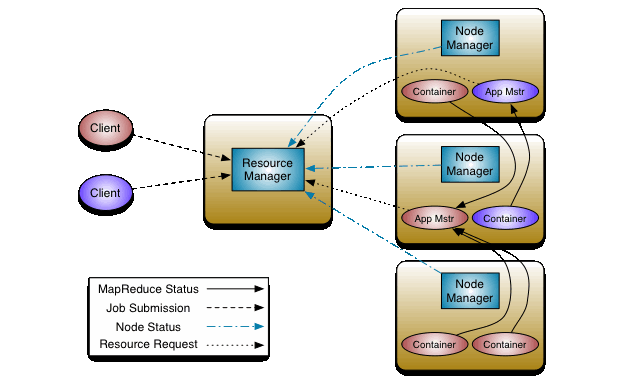
\includegraphics{./resources/yarn_architecture.png}
    \caption[Architektur des YARN"=Frameworks]
    {Architektur des \ac{YARN}"=Frameworks (entnommen aus \cite{HadoopYarnArch271})}
    \label{fig:yarnarch}
\end{figure}

Der \ac{RM} dient hierbei als \emph{Load"=Balancer} für das gesamte Cluster und besteht aus dem \ac{AM} und dem \emph{Scheduler}, die eigentliche Ausführung der Anwendungen findet auf den Nodes statt.
Der \ac{AM} ist für die Annahme und Ausführung von einzelnen Anwendungen zuständig, denen der Scheduler die dafür notwendigen Ressourcen im Cluster zuteilt.
Jeder Node besitzt einen \ac{NM}, der für die Überwachung der Ressourcen auf dem jeweiligen Node sowie der auf dem Node ausgeführten Anwendungs"=Container zuständig ist und diese Daten dem \ac{RM} übermittelt.

Jede \ac{YARN}"=Anwendung bzw. Job besteht aus einer oder mehreren Ausführungsinstanzen, genannt \emph{Attempts}.
Jeder Attempt besitzt einen eigenen \ac{AppMstr}, welcher das Monitoring der Anwendung und die Kommunikation mit dem \ac{RM} und \ac{NM} übernimmt und die dafür benötigten Informationen bereitstellt \cite{HadoopYarnArch271}.
Die eigentliche Ausführung einer Anwendung findet in den bereits erwähnten \emph{Containern} statt, die jeweils einem Attempt zugeordnet sind.
Container können auf einem beliebigen Node ausgeführt werden und repräsentieren die Ausführung eines Tasks innerhalb der Anwendung.

Zu erwähnen ist hier zudem, dass die Kommunikation zwischen den einzelnen Komponenten nicht in allen Fällen in Echtzeit statt findet.
Vor allem das Prüfen des generellen Node"=Zustandes durch den \ac{RM} wird bei einer Standard"=Konfiguration in periodischen Abständen von jeweils mehreren Minuten durchgeführt.
Sollte der \ac{NM} bei solchen Status"=Abfragen zunächst nicht reagieren, wird mehrere Minuten gewartet, bis der Node als defekt erkannt wird.
Ähnlich verhält es sich bei Zustandsabfragen an den \ac{AppMstr} \cite{HadoopYarnConfig271}.

Ein weiterer Bestandteil von Hadoop bzw. \ac{YARN} ist der \ac{TLS}.
Er ist speziell dafür entwickelt, die Metadaten und Logs der \ac{YARN}"=Anwendungen zu speichern und jederzeit, also als Anwendungshistorie, auszugeben \cite{HadoopYarnTlServer271}.

Zum Steuern des Clusters bzw. dem Monitoring der mithilfe von \ac{YARN} ausgeführten Anwendungen stellt Hadoop drei Schnittstellen zur Verfügung.
Dies sind eine graphische Weboberfläche, was zugleich auch die wichtigste Schnittstelle darstellt, entsprechende Befehle für die \acl{CLI} (engl. \emph{Command-line interface}, kurz \acs{CLI})\acused{CLI}, sowie eine REST"=API.
Während sich die Weboberfläche zur menschlichen Interaktion oder zum Finden von Fehlern eignet, dienen die \ac{CLI}"=Befehle vor allem zum Steuern des Clusters und die REST"=API zur automatisierten Rückgabe der Daten des Clusters zur Nutzung in anderen Programmen \cite{HadoopClusterSetup271,HadoopYarnCmds271,HadoopRmApi271,HadoopNmApi271}.

Das \textbf{\ac{HDFS}} basiert auf einer ähnlichen Architektur wie \ac{YARN} und besitzt ebenfalls einen Controller und mehrere Nodes:

\begin{figure}[h]
    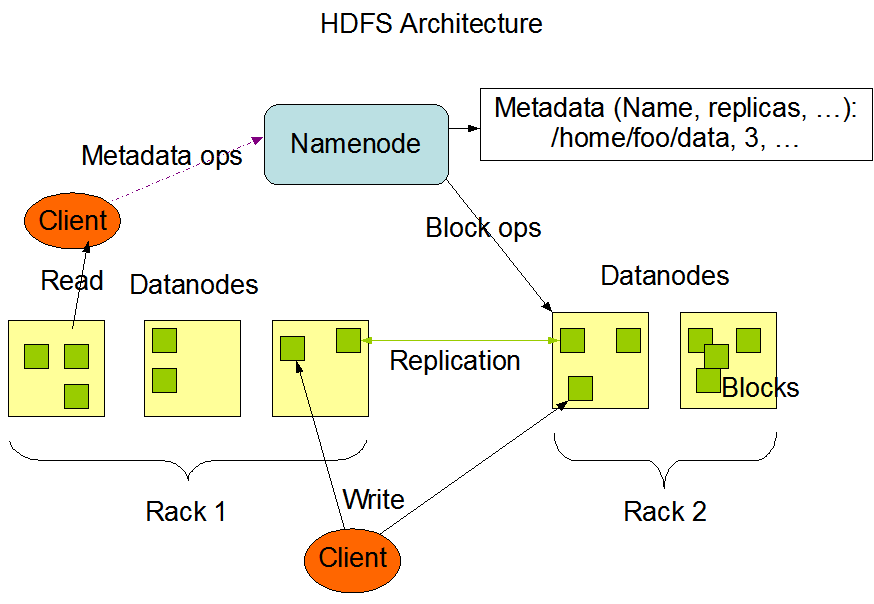
\includegraphics{./resources/hdfsarchitecture.png}
    \caption[Architektur des HDFS]
    {Architektur des \acs{HDFS} (entnommen aus \cite{HadoopHdfsDesc271})}
    \label{fig:hdfsarch}
\end{figure}

Der \emph{NameNode} dient als Controller für die Verwaltung des Dateisystems und reguliert den Zugriff auf die darauf gespeicherten Daten.
Unterstützt wird der NameNode vom \emph{Secondary NameNode}, der Teile der internen Datenverwaltung des \ac{HDFS} durchführt \cite{HadoopHdfsGuide271}.
Die Daten selbst werden in mehreren Blöcke aufgeteilt auf den \emph{DataNodes} gespeichert.
Um den Zugriff auf die Daten im Falle eines Node"=Ausfalls zu gewährleisten, wird jeder Block auf anderen Nodes repliziert.
Dateioperationen (wie Öffnen oder Schließen) werden direkt auf den DataNodes ausgeführt.
Sie sind darüber hinaus auch dafür verantwortlich, dass die gespeicherten Daten gelesen und beschrieben werden können \cite{Shvachko2010,HadoopHdfsDesc271}.

Das Überprüfen der DataNodes durch den NameNode erfolgt genauso wie bei den entsprechenden \ac{YARN}"=Komponenten periodisch im Abstand von mehreren Minuten.
Auch hier dauert es bei einer Standard"=Konfiguration daher mehrere Minuten, bis erkannt wird, wenn ein DataNode nicht mehr verfügbar ist \cite{HadoopHdfsConfig271}.


\section{Adaptive Komponente in Hadoop}
\label{sec:inriaSetting}

Eine normale Hadoop"=Installation besitzt keine Komponente zur dynamischen Anpassungen der Einstellungen des Clusters.
Um damit Hadoop zu optimieren, müssen die Einstellungen daher immer manuell auf den jeweils benötigten Anwendungstyp angepasst werden.
Dazu gibt es \uA verschiedene Scheduler, den \emph{Fair Scheduler}, welcher alle Anwendungen ausführt und ihnen gleich viele Ressourcen zuteilt, und den \emph{Capacity Scheduler}.
Letzterer sorgt dafür, dass nur eine bestimmte Anzahl an Anwendungen pro Benutzter gleichzeitig ausgeführt wird und teilt ihnen so viele Ressourcen zu, wie benötigt werden bzw. dem Benutzer zur Verfügung stehen.
Entwickelt wurde der Capacity Scheduler vor allem für Cluster, die von mehreren Organisationen gemeinsam verwendet werden.
Er soll sicherstellen, dass jede Organisation eine Mindestmenge an Ressourcen zur Verfügung hat \cite{HadoopCapScheduler271}.
Für diesen Scheduler wurde in \cite{Zhang2016} ein selbstadaptiver Ansatz vorgestellt (in dieser Arbeit auch als \textbf{Selfbalancing"=Komponente} bezeichnet), welcher im Folgenden genauer erläutert wird.

\subsection{MARP"=Wert}
\label{subsec:selfbalancingMarp}

Der Capacity Scheduler besitzt verschiedene Einstellungen, um ihn für das konkrete Cluster anzupassen.
So besteht \zB die Möglichkeit, den verfügbaren Speicher pro Anwendungs"=Container festzulegen oder welcher Anteil der verfügbaren Ressourcen durch \gls{AppMstr}"=Container beansprucht werden darf.
Vor allem letztere Einstellungsmöglichkeit Namens \gls{MARP} ist sehr wichtig, wenn mehrere Anwendungen gleichzeitig ausgeführt werden sollen.
Der in der Konfiguration des Schedulers definierte \gls{MARP}"=Wert gibt an, wie viel Prozent des verfügbaren Speichers durch \gls{AppMstr}"=Container genutzt werden darf \cite{HadoopCapScheduler271}.
Der gesamte, für Anwendungen verfügbare Speicher wird durch den \gls{MARP}"=Wert in zwei Teile aufgeteilt.
Während ein Teil des Speichers nur durch \gls{AppMstr}"=Container beansprucht werden darf, wird der andere Teil des Speichers durch alle anderen Anwendungs"=Container genutzt.
Wird durch den \gls{MARP}"=Wert der erste, für \gls{AppMstr}"=reservierten Teil zu klein gehalten, können daher weniger \gls{AppMstr} allokiert werden und somit auch weniger Anwendungen gestartet werden (\emph{Loss of Jobs Parallelism}, LoJP).
Ist der \gls{MARP}"=Wert dagegen zu groß, wird der verfügbare Speicher zu entsprechend großen Teilen für mögliche \gls{AppMstr} reserviert.
Dadurch ist der Anteil des Speichers für Anwendungs"=Container entsprechend klein und es können dadurch weniger Container gestartet werden, um eine Anwendung auszuführen, womit sich die Ausführungsgeschwindigkeit der Anwendungen verringert (\emph{Loss of Job Throughput}, LoJT) \cite{Zhang2016}:

\begin{figure}[h]
    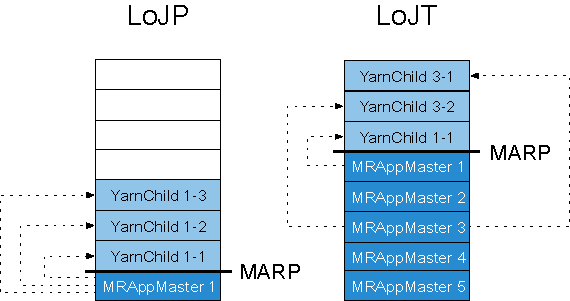
\includegraphics{./resources/marpValue.pdf}
    \caption[LoJP und LoJT in Hadoop]
    {LoJP und LoJT in Hadoop (entnommen aus \cite{Zhang2016}).
        Während beim LoJP sehr viel Speicher für Anwendungs"=Container ungenutzt bleibt, können beim LoJT nicht genügend Anwendungs"=Container allokiert werden, um die Anwendungen auszuführen.}
    \label{fig:marpValue}
\end{figure}

Damit bestimmt der \gls{MARP}"=Wert indirekt auch die maximale Anzahl an Anwendungen, die gleichzeitig ausgeführt werden können.
Da der \gls{MARP}"=Wert jedoch nicht während der Laufzeit dynamisch angepasst werden kann, haben \citeauthor{Zhang2016} in \cite{Zhang2016} einen Ansatz zur dynamischen Anpassung des \gls{MARP}"=Wertes zur Laufzeit von Hadoop vorgestellt.
Die entwickelte Selfbalancing"=Komponente passt den \gls{MARP}"=Wert abhängig von der Speicherauslastung der ausgeführten Anwendungen dynamisch zur Laufzeit an.
So wird der \gls{MARP}"=Wert, und damit auch die Anzahl der ausführbaren \gls{AppMstr}, verringert, wenn die Speicherauslastung sehr hoch ist, und erhöht, wenn die Speicherauslastung sehr niedrig ist.
Die Selfbalancing"=Komponente ermöglicht daher, dass immer die maximal mögliche Anzahl an Anwendungen ausgeführt werden kann.
Die Evaluation von \citeauthor{Zhang2016} ergab zudem, dass Anwendungen dadurch im Schnitt um bis zu 40 Prozent schneller ausgeführt werden können.
Zudem kann die dynamische Anpassung auch effizienter sein, als eine manuelle, statische Optimierung \cite{Zhang2016}.

\subsection{Analyse der Selfbalancing"=Komponente}
\label{subsec:selfbalancingAnalysis}

Da in dieser Fallstudie auch Mutationstests eingesetzt werden, bei denen die Selfbalancing"=Komponente entsprechend verändert wird (Implementierung in \cref{sec:implMutationTests}), wurde die Komponente zunächst analyisiert.
Sie besteht aus folgenden vier Java"=Klassen, welche den Kern der Komponente darstellen, und drei Shell"=Scripten, die als Verbindung zum Hadoop"=Cluster dienen:

\begin{itemize}
    \item Java"=Klassen:
    \begin{itemize}
        \item \texttt{controller.Controller}
        \item \texttt{effectuator.Effectuator}
        \item \texttt{monitor.ControlNodeMonitor}
        \item \texttt{monitor.MemUtilization}
    \end{itemize}
    \item Shell"=Scripte:
    \begin{itemize}
        \item \texttt{selfTuning-CapacityScheduler.sh}
        \item \texttt{selfTuning-controlNode.sh}
        \item \texttt{selfTuning-mem-controlNode.sh}
    \end{itemize}
\end{itemize}

Um den Zustand von Hadoop korrekt zu ermitteln, wird ein Kalman"=Filter in Form der Open"=Source"=Bibliotek JKalman\footnote{\url{https://jkalman.sourceforge.io/}} genutzt.
Der Kalman"=Filter wurde von \citeauthor{Kalman1960} erstmals in \cite{Kalman1960} beschrieben und wird genutzt, um \enquote{aus verrauschten und teils redundanten Messungen die Zustände und Parameter des Systems zu schätzen} \cite{Marchthaler2017}.
Der Filter lässt sich aufgrund seines Aufbaus zudem auch für Echtzeitanwendungen nutzen \cite{Marchthaler2017}.
Als einfaches Anwendungsbeispiel hierfür ist in \cite{Marchthaler2017} die Apollo"=Mondlandefähre genannt, \citeauthor{Strukov2001} nutzte ihn in \cite{Strukov2001} aber auch zur Reduktion der Komplexität im Controlling.
Für weitere Informationen zum Kalman"=Filter wie seinen Aufbau, Funktionsweise und Anwendung sei hier auf entsprechende Fachliteratur wie \zB \cite{Kim2016,Simon2006,Aggoun2004} verwiesen.

Die drei Shell-Scripte der Selfbalacing"=Komponente dienen zur Interaktion zwischen der Komponente und dem Cluster.
Die beiden zuletzt genannten Scripte werden von den beiden Monitor"=Klassen sekündlich gestartet und ermitteln basierend auf den Logs von Hadoop die Auslastung des Clusters.
Mithilfe von \texttt{selfTuning-controlNode.sh}, das von \texttt{ControlNodeMonitor} gestartet wird, wird die Anzahl an aktiven und wartenden YARN"=Jobs ermittelt und anschließend in der \texttt{controlNodeLog}"=Datei gespeichert.
Durch die Ausführung von \texttt{selfTuning-mem-controlNode.sh} (gestartet durch \texttt{MemUtilization}) wird dagegen die Auslastung des Speichers des Clusters ermittelt und in der \texttt{memLog}"=Datei notiert.

Die in den beiden Dateien enthaltenen Werten werden im Anschluss wiederum sekündlich vom \texttt{Controller} der Selfbalancing"=Komponente ausgelesen und mithilfe des Kalman"=Filters bereinigt.
Anschließend werden die Algorithmen \cite{Zhang2016} zum Berechnen des neuen \gls{MARP}"=Wertes ausgeführt.

Um den dadurch neu ermittelten \gls{MARP}"=Wert anzuwenden, wird abschließend mithilfe des \texttt{Effectuator}s das dritte Shell"=Script \texttt{selfTuning-CapacityScheduler.sh} ausgeführt.
Mithilfe dieses Shell"=Scriptes wird der neue MARP"=Wert in der Konfiguration des \emph{Capacity Schedulers} gespeichert.


\section{Plattform Hadoop"=Benchmark}
\label{sec:hadoopBenchmark}

\citeauthor{Zhang2016} haben im Rahmen ihrer gesamten Forschungsarbeit an der Selfbalancing"=Komponente darüber hinaus auch die Open"=Source"=Plattform Hadoop"=Benchmark entwickelt\footnote{\url{https://github.com/Spirals-Team/hadoop-benchmark}}.
Sie dient zur einfachen und schnellen Ausführung eines Hadoop"=Clusters und wurde speziell zum Einsatz in der Forschung erstellt.
Dadurch kann sie auch mit geringem Aufwand an eigene Bedürfnisse angepasst werden.

Zur Ausführung des Clusters wird die Virtualisierungs"=Software Docker\footnote{\url{https://www.docker.com/}} und das dazugehörige \emph{Docker Machine} genutzt.
Durch die Virtualisierung wird für jeden Hadoop"=Node eine Docker"=Machine gestartet, auf der der Hadoop"=Node wiederum in einem Docker"=Container ausgeführt wird.
Verbunden werden die Nodes dabei mithilfe eines \emph{Docker" Swarm}s\footnote{\url{https://docs.docker.com/engine/swarm/}}.

\begin{figure}[h]
    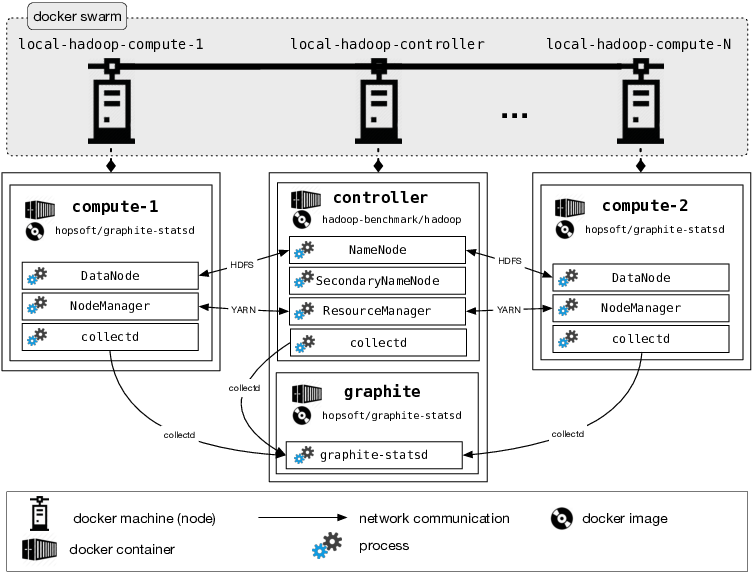
\includegraphics{./resources/hadoopBenchmarkArch.png}
    \caption[High"=Level"=Architektur von Hadoop"=Benchmark]
    {High"=Level"=Architektur von Hadoop"=Benchmark (entnommen aus \cite{abb:hadoopBenchmarkArch})}
    \label{fig:hadoopBenchmarkArchitecture}
\end{figure}

Docker"=Machine ist keine komplette Virtualisierungs"=Software, sondern nutzt hier VirtualBox\footnote{\url{https://www.virtualbox.org/}}, um virtuelle Maschinen zu starten, die mit dem Betriebssystem \emph{Boot2Docker} ausgestattet sind.
Boot2Docker ist eine leichtgewichtige Linux"=Distribution, auf der Docker bereits vorinstalliert ist \cite{DockerMachineGettingStartedVm}.

Mit \emph{Graphite}\footnote{\url{https://graphiteapp.org/}} ist zudem ein Monitoring"=Tool enthalten, mit dem die Systemwerte wie CPU- oder Speicher"=Auslastung des Clusters überwacht und analysiert werden kann.
Jeder Hadoop"=Container enthält dazu das Tool \emph{collectd}\footnote{\url{https://collectd.org/}}, was das Monitoring des Containers auf Systemebene übernimmt und die Daten an den Graphite"=Container übermittelt.

Da mithilfe der Plattform auch unterschiedliche Hadoop"=Konfigurationen ausgeführt werden können, ist die Plattform in mehrere Szenarien unterteilt.
Jedes Szenario stellt eine Hadoop"=Konfiguration dar, die vollständig angepasst werden kann.
Jedes Szenario enthält daher eine \emph{Dockerfile}, aus der die Docker"=Images und -Container erstellt werden, weitere für Hadoop benötigte Daten und Einstellungen, sowie dazugehörige generelle Einstellungen des Szenarios.
Die Plattform enthält bereits mehrere Szenarien, \uA Hadoop in der Version 2.7.1 ohne Anpassungen sowie ein darauf basierendes Szenario mit der Selfbalancing"=Komponente.
Aufgrund eines der Kernkonzepte von Docker, wonach Docker"=Images auf einem passenden, bereits vorhandenen Images aufbauen können bzw. sollten \cite{DockerdevBestPractice}, ist es möglich, neue Szenarien basierend auf bereits vorhandenen zu entwickeln.

Zum Starten des Clusters ist ein Script enthalten, welches basierend auf dem zu nutzenden Szenario das Cluster in der entsprechenden Konfiguration startet.

In der Plattform Hadoop"=Benchmark sind auch bereit einige Benchmarks integriert:

\begin{itemize}
    \item Hadoop Mapreduce Examples
    \item Intel HiBench\footnote{\url{https://github.com/intel-hadoop/HiBench}}
    \item \gls{SWIM} \footnote{\url{https://github.com/SWIMProjectUCB/SWIM}}
\end{itemize}

Die Benchmarks werden ebenfalls mithilfe der in der Plattform enthaltenen Scripte gestartet.
Hierbei besitzt jeder Benchmark ein eigenes Start"=Script, das den Benchmark in einem Docker"=Container startet und die entsprechende \gls{Anwendung} so dem Cluster zur Ausführung übergibt.
Die Ausführung einer \gls{Anwendung} mithilfe des entsprechenden Start"=Scriptes sowie das Beenden einer \gls{Anwendung} ist in \cref{app:hadoopCmds} beispielhaft aufgezeigt.

Genauere Informationen zu den in der Plattform enthaltenen Benchmarks sind in \cref{sec:appOverview} erläutert.


    \chapter{Aufbau und Ablauf der Fallstudie}
\label{chap:caseStudy}

Im Rahmen dieser Masterarbeit soll nun mithilfe von Hadoop und der Selfbalancing"=Komponente eine Fallstudie durchgeführt werden, durch die ermittelt wird, unter welchen Umständen eine Testautomatisierung möglich ist.
\todo{Ergebnis zur Frage zur Testautomatistierung in Reflexion}
Hierfür werden mehrere Anforderungen an das durch den grundlegenden Versuchsaufbau definierte Modell gestellt.
Dieses Modell wird zur Realisierung der Tests mithilfe des \ac{ss}"=Frameworks als ein vereinfachtes Modell von Hadoop entwickelt und mit einem realen Cluster verbunden.

Teile der Beiträge und Inhalte dieses Kapitels wurden bereits in \cite{Eberhardinger2018} publiziert.

\section{Grundlegender Versuchsaufbau}
\label{sec:clusterSetup}

Neben den Anforderungen an Hadoop und das gesamte Testsystem muss auch der grundlegende Versuchsaufbau in dieser Fallstudie definiert werden.
Im Grunde wird, wie bereits in \autoref{chap:intro} erwähnt, Hadoop mithilfe des \ac{ss}"=Frameworks nachgebildet und dieses Modell mit einem realen Cluster verbunden.
\todo{dort erwähnen}
In diesem Cluster sollen anhand des Modells unterschiedliche Komponentenfehler injiziert und repariert werden, als auch unterschiedliche Benchmarks gestartet werden.
Hierbei soll nicht nur das Verhalten von Hadoop selbst analysiert werden, sondern auch das der von \citeauthor{zhang2016} entwickelten Selfbalancing"=Komponente.
Anhand dieses Verhaltens und dem des kompletten Testsystems soll schließlich ermittelt werden, ob eine Testautomatisierung in diesem Versuchsaufbau erfolgreich war.

Bei der Entwicklung des Modells liegt der Fokus auf dem grundlegenden Aufbau von \ac{YARN}.
Dazu gehören die Anwendungen und ihre Attempts, sowie zum Teil auch ihre Container.
Daneben muss das Modell auch die Nodes des Clusters und zum Ausführen der Benchmarks auch simulierte Clients enthalten.
Da bei den Tests auch Ausfälle von Nodes eine Rolle spielen, müssen hierfür entsprechende Komponentenfehler implementiert werden, die mithilfe von \ac{ss} aktiviert und deaktiviert werden können.

Da die Auswahl der ausgeführten Benchmarks eines jeden Clients nicht bei jedem Test manuell bestimmt werden soll, wird hierfür ein Transitionssystem verwendet.
Mithilfe dieses Transitionssystems, in dem die Wahrscheinlichkeiten von Wechseln zwischen zwei Anwendungen definiert sind, soll während der Ausführung eines Testfalls zufällig eine nachfolgende Anwendung ausgewählt werden.
%Da zum Testen des Clusters der \ac{ss}"=Simulator eingesetzt wird, hängt die Anzahl der Anwendungen primär von der Anzahl der ausgeführten Simulations"=Schritte ab.
%Ein weiterer Faktor zur Anzahl der Anwendungen ist die Anzahl an simulierten Clients, da auch getestet werden soll, wie sich das Cluster bei der Ausführung von mehreren parallel gestarteten Anwendungen verhält.

Die Verbindung zwischen dem Modell und dem realen Hadoop"=Cluster wird mithilfe eines dafür entwickelten Treibers durchgeführt.
Der Treiber ist dafür verantwortlich, Komponentenfehler und Anwendungen an das reale Cluster zu senden.
Zudem dient er dazu, um den Status des Clusters jederzeit ermitteln und an das Modell zur dortigen Speicherung übergeben zu können.
Er kann daher nicht nur aus der Verbindung zum Cluster selbst bestehen, sondern muss auch die Kommunikation zwischen Modell und Cluster sicherstellen und übermittelte Daten entsprechend umwandeln.

Zur Umsetzung des realen Clusters wird die von \citeauthor{zhang2016} entwickelte Plattform Hadoop"=Benchmark mit für diese Fallstudie entwickelten Szenarios genutzt.
Als Basis dient hierzu das bereits in der Plattform enthaltene Szenario mit der Nutzung der Selfbalancing"=Komponente.
Zudem soll auch mithilfe von Mutationstests, bei denen einer oder mehrere Mutanten in der Selfbalancing"=Komponente implementiert werden, das Testsystem geprüft werden.

Dieser Versuchsaufbau soll zudem mithilfe eines dafür entwickelten \emph{Oracles} geprüft werden.
Das Oracle dient zur Validierung der in \autoref{sec:requirements} definierten Anforderungen an das Cluster und das Testsystem.
Hierfür werden, sofern möglich, die Anforderungen als \emph{Constraints} im Modell implementiert und bei jedem Test automatisch geprüft.

Die Implementierung des eben beschriebenen Modells und Oracles ist im \autoref{chap:modell} beschrieben.
Die Auswahl der verwendeten Benchmarks und deren Implementierung mit dem Transitionssystem findet sich in \autoref{chap:benchmarks}.


\section{Anforderungen an das Cluster und Testsystem}
\label{sec:requirements}

Zur Überprüfung des Clusters und des Testssystems selbst werden hierfür jeweils mehrere Anforderungen gestellt.
Unterschieden wird hierbei zwischen funktionalen Anforderungen an das \gls{SuT} und Anforderungen an das Testsystem.
Während die funktionalen Anforderungen ausschließlich vom Hadoop"=Cluster als \gls{SuT} erfüllt werden müssen, müssen die Test"=Anforderungen vom gesamten Testsystem erfüllt werden.

Mithilfe der im Folgenden definierten Anforderungen soll bereits automatisiert geprüft werden, inwieweit eine Testautomatisierung möglich ist.
Hierfür werden die Anforderungen, sofern möglich, in Form von Constraints ebenfalls im Modell implementiert und während der Ausführung durch das Oracle validiert.

\subsection{Funktionale Anforderungen an das Cluster}
\label{subsec:functionalRequirements}

Obwohl in dieser Masterarbeit der Fokus auf Testautomatisierung und Validieren eines Testsystems liegt, müssen auch die funktionalen Anforderungen an das \gls{SuT}, also das Hadoop"=Cluster selbst, berücksichtigt werden.
Da im Rahmen der Publikation \cite{Eberhardinger2018} ebenfalls der in \cref{sec:clusterSetup} beschriebene, und in dieser Fallstudie genutzte Versuchsaufbau genutzt wurde, wurden im Rahmen dieser Fallstudie auch funktionale Anforderungen an das Cluster selbst durch das Oracle geprüft.
Dies betrifft konkret folgende Anforderungen an das \gls{SuT} \cite{Eberhardinger2018}:

\begin{enumerate}
    \item Ein Task wird vollständig ausgeführt, sofern er nicht abgebrochen wird
    \item Kein Task oder Anwendung wird an inaktive, defekte oder nicht verbundene Nodes gesendet
    \item Die Konfiguration wird aktualisiert, sobald eine entsprechende Regel erfüllt ist
    \item Defekte oder Verbindungsabbrüche werden erkannt
\end{enumerate}

\subsection{Anforderungen an das Testsystem}
\label{subsec:testRequirements}

Neben den funktionalen Anforderungen, gibt es weitere Anforderungen an das gesamte Testsystem.
Diese Anforderungen betreffen das Hadoop"=Cluster, die Selfbalancing"=Komponente, das entwickelte \gls{ss}"=Modell sowie den Treiber zur Kommunikation zwischen Modell und Cluster.
Konkret sind dies folgende Anforderungen an das Testsystem:

\begin{enumerate}
    \item Der \gls{MARP}"=Wert ändert sich, basierend auf den derzeit ausgeführten Anwendungen
    \item Der jeweils aktuelle Status des Clusters wird erkannt und im Modell gespeichert
    \item Defekte Nodes und Verbindungsabbrüche werden erkannt
    \item Im Modell implementierte Komponentenfehler werden im realen Cluster injiziert und repariert
    \item Wenn alle Nodes defekt sind, wird erkannt, dass sich das Cluster nicht mehr rekonfigurieren kann
    \item Ein Test kann vollautomatisch ausgeführt werden
    \item Das Cluster kann ohne Auswirkungen auf seine Funktionsweise auf einem oder mehreren Hosts ausgeführt werden
    \item Es können mehrere Benchmark"=Anwendungen gleichzeitig gestartet und ausgeführt werden
    \item Tests und Testfälle können zeitlich unabhängig und mehrmals ausgeführt werden
\end{enumerate}

Die funktionalen Anforderungen dienen zudem ebenfalls als Anforderungen an das Testsystem und erweitern somit die hier genannten Anforderungen.

Eine Besonderheit bildet die fünfte Anforderung, wonach erkannt werden muss, dass im Cluster keine weitere Rekonfiguration möglich ist.
Wird diese Anforderung verletzt, soll der ausgeführte Test abgebrochen werden, während bei den anderen, auch den funktionalen, Anforderungen dies nur durch das Oracle vermerkt, die Ausführung aber nicht weiter beeinträchtigt werden soll.


\section{Anforderungen an das Testsystem}
\label{sec:evaluationPlan}

Um das Testsystem zu validieren, wurde zunächst ein Evaluationsplan aufgestellt.
In diesem ist festgehalten, was getestet wird, wie die Testfälle aussehen und wie die bei der Ausführung gewonnen Daten organisiert werden.

\subsection{Behauptungen und Variablen}
\label{sec:predictions}

% Was für Behauptungen wurden aufgestellt
\begin{enumerate}
    \setcounter{enumi}{4}
    \item Der jeweils aktuelle Status des Clusters wird erkannt und im Modell gespeichert
    \item Defekte Nodes und Verbindungsabbrüche werden erkannt
    \item Im Modell implementierte Komponentenfehler werden im realen Cluster injiziert und repariert
    \item Wenn alle Nodes defekt sind, wird erkannt, dass sich das Cluster nicht mehr rekonfigurieren kann
    \item Ein Test kann vollautomatisch ausgeführt werden
    \item Das Cluster kann ohne Auswirkungen auf die Funktionsweise auf einem oder beiden Hosts ausgeführt werden
    \item Es können mehrere Benchmark"=Anwendungen gleichzeitig gestartet und ausgeführt werden
    \item Ein Testfall kann zeitlich unabhängig und mehrmals ausgeführt werden
\end{enumerate}

% Was für Variablen wurden dadurch ermittelt

\subsection{Generierung der Testfälle}
\label{sec:testcaseGeneration}

Die Generierung der Testfälle hängt von mehreren Faktoren ab.
Zum einen ist ein Testfall abhängig von der Größe des Clusters, also ob das Cluster auf einem oder beiden Hosts ausgeführt wird und aus wie vielen Nodes das Cluster besteht.
Relevant zur Unterscheidung von Testfällen sind aber auch die ausgeführten Anwendungen.
Da die Auswahl der ausgeführten Anwendungen nicht manuell bestimmt werden soll, wird hierfür ein Transitionssystem verwendet.
Mithilfe dieses Transitionssystems, in dem die Wahrscheinlichkeiten von Wechsel zwischen zwei Anwendungen definiert sind, soll während der Ausführung eines Testfalls zufällig eine nachfolgende Anwendung ausgewählt werden.
Da zum Testen des Clusters der \ac{ss}"=Simulator eingesetzt wird, hängt die Anzahl der Anwendungen primär von der Anzahl der ausgeführten Simulations"=Schritte ab.
Ein weiterer Faktor zur Anzahl der Anwendungen ist die Anzahl an simulierten Clients, da auch getestet werden soll, wie sich das Cluster bei der Ausführung von mehreren parallel gestarteten Anwendungen verhält.
Die zu injizierenden Komponentenfehler, mit denen defekte Nodes und Verbindungsausfälle simuliert werden, werden ebenfalls zufallsbasiert ausgewählt.
Dies gilt auch für das Deaktivieren der Komponentenfehlern.

Die Auswahl der nachfolgenden Anwendungen und die Entscheidung über die Aktivierung und Deaktivierung der Komponentenfehlern wird daher mithilfe eines Zufallsgenerators realisiert.
Hierbei soll jedoch kein echter Zufallsgenerator zum Einsatz kommen, sondern ein Pseudo"=Zufallsgenerator.
Da ein Pseudo"=Zufallsgenerator seine Werte mithilfe eines Start"=\emph{Seeds} auswählt, besteht somit die Möglichkeit durch die Verwendung eines bestimmten Seeds, einen Testfall jederzeit wiederholen zu können.
Zur Auswahl der ersten Testfälle werden daher zeitbasierte Seeds verwendet.
Diese Seeds werden bei der Ausführung notiert und für andere Testfälle verwendet, bei denen andere Punkte der Konfiguration wie \zB die Größe des Clusters, abgeändert werden.
Dadurch ist es möglich, die Auswirkungen einzelner Parameter zu testen und zu evaluieren.
\todo{Wo wird Seed wie genutzt? am besten in implementierung davon!}

\subsection{Organisation und Ausgabe der Daten}
\label{sec:dataOrganisation}

Damit die bei der Ausführung gewonnenen Daten auch zur Evaluation genutzt werden können, wurde hierzu festgelegt, welche Daten während der Ausführung ausgegeben werden.
Alle relevante Daten werden hierzu während der Ausführung der Testfälle in einer Log"=Datei gespeichert.
Zur Unterscheidung von einzelnen Ausführungen werden die Daten klar strukturiert.
Neben den im folgenden beschriebenen Daten werden zudem alle Ein- und Ausgabedaten der SSH"=Verbindungen zwischen \ac{ss} und dem Cluster (vgl. \autoref{sec:aufbauCluster}) in einem eigenen Log gespeichert.

Beim Start der Simulation werden zunächst einige generelle Daten ausgegeben:

\begin{itemize}
    \item Basis"=Seed für die Zufallsgeneratoren
    \item Mindestdauer für einen Simulations"=Schritt
    \item Anzahl der ausgeführten Simulations"=Schritte
    \item Wahrscheinlichkeiten für Aktivierung und Deaktivierung der Komponentenfehler
    \item Angabe, ob vorab generierte Eingabedaten genutzt werden oder diese während der Ausführung eines Testfalls generiert werden
    \item Anzahl genutzter Hosts und Nodes
    \item Pfade verwendeter Scripte auf den Hosts (vgl. \autoref{sec:aufbauCluster})
    \item Bei der Nutzung der REST"=API verwendete URL des Controllers
    \item Auszuführende Benchmarks    
\end{itemize}

Die Ausgabe der Daten der YARN"=Komponenten wird bei jedem Simulations"=Schritt durchgeführt, damit das Verhalten des Clusters berücksichtigt werden kann.
Ausgegeben werde hierbei:

\begin{itemize}
    \item Für jeden Node:
    \begin{itemize}
        \item ID bzw. Name des Nodes
        \item Aktueller Status
        \item Informationen zur Fehleraktivierung
        \item Anzahl ausgeführter Container auf dem Node
        \item Angaben zur Speicherauslastung
        \item Angaben zur CPU"=Auslastung
    \end{itemize}
    
    \item Für jeden Client:
    \begin{itemize}
        \item ID bzw. Name des Clints
        \item Aktuell ausgeführter Benchmark
        \item ID der aktuell ausgeführten Anwendung auf dem Cluster
    \end{itemize}

    \item Für jede Anwendung:
    \begin{itemize}
        \item ID der Anwendung
        \item Bezeichnung der Anwendung
        \item Aktueller und finaler Status der Anwendung
        \item ID bzw. Name des Nodes, auf dem der \ac{AppMstr} ausgeführt wird
    \end{itemize}

    \item Für jeden Attempt:
    \begin{itemize}
        \item ID des Attempts
        \item Aktueller Status des Attempts
        \item ID des \ac{AppMstr}"=Containers
        \item ID bzw. Name des Nodes, auf dem der \ac{AppMstr} ausgeführt wird
    \end{itemize}

    \item Für jeden Container:
    \begin{itemize}
        \item ID des Containers
        \item ID bzw. Name des auszuführenden Nodes
        \item Aktueller Status des Containers
    \end{itemize}
\end{itemize}

Die Details zur Implementierung und dem Ausgabeformat sind in \autoref{sec:simulationStepOutput} erläutert.


    \chapter{Aufbau des Modells}\label{chap:model}

\section{Grundlegende Architektur}\label{sec:architecture}

\begin{wrapfigure}{r}{0.5\columnwidth}
	\centering
	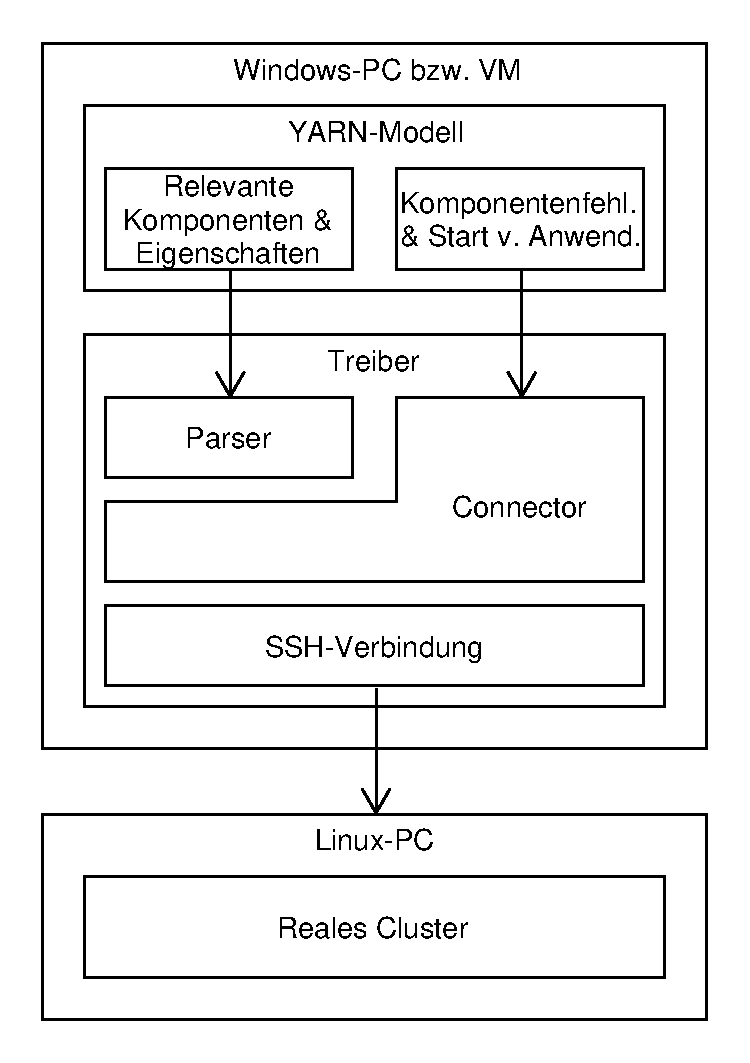
\includegraphics[width=0.5\columnwidth]{./images/modelArchitecture.pdf}
	\caption{Grundlegende Architektur des Gesamtmodells}
	\label{fig:modelArchitecture}
\end{wrapfigure}

Die grundlegende Architektur des gesamten Aufbaus besteht aus den drei in \autoref{fig:modelArchitecture} zu sehenden Schichten. Die oberste Schicht bildet dabei das \sS-Modell von Hadoop YARN, welches die wesentlichen YARN-Komponenten und dessen Komponentenfehler abbildet. Das reale Pendant dazu bildet das reale Cluster als unterste Schicht. Die Verbindung zwischen dem Modell und dem realen Cluster bildet der Treiber als eigenständige Schicht, bestehend aus den Kernkomponenten Parser, Connector und der eigentlichen SSH-Verbindung zum realen Cluster. Da \sS auf dem .NET-Framework aufbaut, ist für den \sS-MC entsprechend ein Windows dafür nötig, während das reale Cluster auf einem eigenen Linux-PC ausgeführt wird, weshalb als Konsequenz zur Kommunikation zwischen Modell und Cluster eine SSH-Verbindung nötig ist.

\section{\sS-Modell}\label{sec:sSharpModel}



\section{Reales Hadoop-System}\label{sec:realHadoop}



\section{SSH-Treiber}\label{sec:sshDriver}

Im Einführungstext zu diesem Kaptiel wurde bereits auf den grundlegenden Aufbau des Treibers eingegangen. Der SSH-Treiber besteht aus den drei einzelnen Komponenten Parser, Connector und SSH-Verbindung, von denen die ersten beiden mithilfe von Interfaces im YARN-Modell eingebunden sind. Dadurch ist es möglich, unterschiedliche Parser bzw. auch Verbindungen für unterschiedliche Komponenten zu nutzen.

Der Parser selbst besteht neben dem eigentlichen Parser zudem aus Datenhaltungs-Klassen für die relevanten YARN-Komponenten. Sie dienen dazu, die geparsten Rohdaten von Hadoop an das \sS-Modell zu übergeben und sind daher ebenfalls mithilfe von entsprechenden Interfaces im Modell eingebunden. Die Implementierungen der Klassen selbst sind außerdem so aufgebaut, dass sie für beide hier implementierten Parser genutzt werden können.

\subsection{Kommandozeilen-Parser}\label{sec:cmdParser}

% Was gibt Hadoop aus
Hadoop besitzt zur Steuerung einige Kommandozeilen-Befehle, mit denen \uA auch die Daten der YARN-Komponenten ausgelesen werden können. Die Daten werden mithilfe der Befehle immer vom \ac{RM} und, sofern gestartet, vom Timeline-Server ermittelt und ausgegeben. Ausgegeben werden können \uA die Daten zu:

\begin{description}[noitemsep]
    \item[Anwendungen] als nach dem Status gefilterte Liste oder der Report einer Anwendung
    \item[Ausführungen] als Liste aller Ausführungen einer Anwendung oder der Report einer Ausführung
    \item[Container] als Liste aller Container einer Ausführung oder der Report eines Containers
    \item[Nodes] als Liste aller Nodes oder der Report eines Nodes
\end{description}

Einige Beispiele für die dafür notwendigen Befehle sowie deren mögliche Ausgaben sind in \autoref{app:hadoopCmds} zu finden.

% Wie wurde der Parser aufgebaut

\subsection{REST-API-Parser}\label{sec:restParser}

% Was gibt Hadoop aus
% Wie wurde der Parser aufgebaut

\subsection{Connector}\label{sec:Connector}

% Wie wird die Verbindung abstrahiert

\subsection{SSH-Verbindung}\label{sec:sshConnection}

% Wie funktioniert die Verbindung selbst

    \chapter{Implementierung der Benchmarks}
\label{ch:benchmarks}

Neben dem \gls{YARN}"=Modell selbst sind auch die während der Testausführung genutzten \glspl{Anwendung} ein wichtiger Bestandteil des gesamten Testmodells.
Da Hadoop selbst sowie die Plattform Hadoop"=Benchmark bereits einige \glspl{Anwendung} und Benchmarks enthalten, konnten diese auch im Rahmen dieser Fallstudie genutzt werden.
Dazu wurde eine Auswahl an \glspl{Anwendung} in einer Markow"=Kette miteinander verbunden, mit dem die Ausführungsreihenfolge der einzelnen \glspl{Anwendung} basierend auf Wahrscheinlichkeiten bestimmt wird.
Verwaltet werden die implementierten Benchmarks mithilfe des Benchmark"=Controllers.

Da für die in \cite{Eberhardinger2018} durchgeführte Fallstudie das für diese Fallstudie entwickelte Testmodell genutzt wurde, enthält es auch das hierfür entwickelte Transitionssystem.
Daher wurden Teile der Beiträge dieses Kapitels dort bereits publiziert.

\section{Übersicht möglicher Anwendungen}\label{sec:appOverview}

Hadoop-Benchmark enthält bereits die Möglichkeit, unterschiedliche Benchmarks zu starten. Wie in \autoref{sec:hadoopBenchmark} erwähnt, sind folgende Benchmarks in der Plattform integriert:

\begin{itemize}
    \item Hadoop Mapreduce Examples
    \item Intel HiBench
    \item \ac{SWIM}
\end{itemize}

Jeder Benchmark enthält zum Starten ein jeweiliges Start"=Script, mit dem ein neuer Docker"=Container auf der Controller"=VM gestartet wird, mit dem der Benchmark auf dem Cluster gestartet wird. Dass dafür ein eigener Docker-Container genutzt wird liegt daran, dass es in Docker"=Umgebungen \emph{best practice} ist, einen Docker"=Container für nur einen Einsatzzweck zu erstellen und zu nutzen. Die Hauptgründe dafür sind, dass dadurch die Skalierbarkeit erhöht und die Wiederverwendbarkeit gesteigert werden \cite{DockerBestPractice}. Daher wurden auch die Startscripte für die Benchmarks so angepasst, dass die jeweiligen Benchmarks mehrfach gestartet werden können.

Die \textbf{Hadoop Mapreduce Examples} sind unterschiedliche und meist voneinander unabhängige Anwendungen, die beispielhaft für die meisten Anwendungsfällen in einem produktiv genutzten Cluster sind. Die Examples sind Teil von Hadoop und daher bei jeder Hadoop"=Installation enthalten. Einige der Anwendungen der Examples sind:

\begin{itemize}
    \item Generatoren für Text und Binärdaten, \zB \acl{rtw}
    \item Analysieren von Daten, \zB \acl{wc}
    \item Sortieren von Daten, \zB \acl{sort}
    \item Ausführen von komplexen Berechnungen, \zB \emph{Bailey-Borwein-Plouffe-Formel} zur Berechnung einzelner Stellen von $\pi$
\end{itemize}

\textbf{Intel HiBench} ist eine Benchmark-Suite mit \emph{Workloads} zu verschiedenen Anwendungszwecken mit jeweils unterschiedlichen einzelnen Anwendungen. Da in Hadoop"=Benchmark noch die HiBench"=Version \mbox{2.2} verwendet wird, wurde der Docker"=Container von HiBench zunächst auf Version 7 aktualisiert, die einige neuen Workloads und Anwendungen enthält. HiBench enthält damit folgende Workloads mit einer unterschiedlichen Anzahl an möglichen Anwendungen:

\begin{itemize}
    \item Micro"=Benchmarks (basieret auf den Mapreduce"=Examples und den Jobclient"=Tests)
    \item Maschinelles Lernen
    \item SQL/Datenbanken
    \item Websuche
    \item Graphen
    \item Streaming
\end{itemize}

\textbf{\ac{SWIM}} ist eine Benchmark-Suite, die aus 50 verschiedenen Workloads besteht. Das besondere dabei ist, dass die dabei verwendeten Mapreduce"=Jobs anhand mehrerer tausend Jobs erstellt wurden und im Vergleich zu anderen Benchmarks eine größere Vielfalt an Anwendungen und somit ein größerer Testumfang gewährleistet wird \cite{SwimWikiHome}. Bei der Ausführung auf dem in dieser Arbeit verwendete Cluster wurden jedoch nicht alle Workloads fehlerfrei ausgeführt. Zudem wird in \cite{InriaTutorial} explizit erwähnt, dass es bei der Ausführung auf einem Cluster auf einem einzelnen PC bzw. Laptop Probleme geben kann. Zudem ist SWIM für Benchmarks eines Clusters mit mehreren physischen Nodes ausgelegt ist und daher würde die Ausführung in dieser Fallstudie extrem viel Zeit benötigten. Daher wurde die Nutzung des SWIM-Benchmarks nicht weiter verfolgt.

Ebenfalls im Installationsumfang von Hadoop enthalten sind die sog. \textbf{Jobclient"=Tests}. Hauptbestandteil dieser Tests sind vor allem weitere Benchmarks, welche das gesamte Cluster oder einzelne Nodes testen, wobei die meisten Anwendungen das \ac{HDFS} betreffen. Da die Jobclient-Tests kein Teil von Hadoop"=Benchmark sind, wurde zur Ausführung der Jobclient"=Test zunächst ein eigenes Start"=Script analog zur Ausführung der Mapreduce"=Examples erstellt, damit hierfür ebenfalls ein eigener Docker"=Container gestartet wird. Die Jobclient"=Tests enthalten \uA folgende Arten an Anwendungen:

\begin{itemize}
    \item \ac{HDFS}"=Systemtests, \zB \texttt{SilveTest}
    \item Reine Lastgeneratoren, \zB \texttt{NNloadGenerator}
    \item Eingabe/Ausgabe"=Durchsatz"=Tests, \zB \texttt{TestDFSIO}
    \item Dummy"=Anwendungen \texttt{sleep} (blockiert Ressourcen, führt aber nichts aus) und \texttt{fail} (Anwendung schlägt immer fehl)
\end{itemize}

\section{Auswahl der verwendeten Anwendungen}
\label{sec:appSelection}

Damit die Fallstudie die Realität abbilden kann, wurden von allen verfügbaren Anwendungen einige ausgewählt und in ein Transitionssystem in Form einer Markow"=Kette überführt.
Diese Kette definiert die Ausführungsreihenfolge zwischen den einzelnen Anwendungen.
Eine zufallsbasierte Markow"=Kette wurde aus dem Grund verwendet, dass auch in der Realität Anwendungen nicht immer in der gleichen Reihenfolge ausgeführt werden und daher auch in der Fallstudie eine unterschiedliche Ausführungsreihenfolge der Anwendungen gewährleistet werden soll.
Mithilfe der Festlegung eines bestimmten Seeds für den in der Fallstudie benötigten Pseudo"=Zufallsgenerator besteht bei Bedarf dennoch die Möglichkeit, einen Test mit den gleichen Anwendungen wiederholen zu können.

Einige der in \cref{sec:appOverview} erwähnten Mapreduce Examples werden häufig als Benchmark verwendet.
Einige Beispiele dafür sind die Anwendungen \acl{so} und \texttt{grep}, die bereits im Referenzpapier des \ac{MR}"=Frameworks zum Testen genutzt wurden \cite{Dean2004}.
Zum Testen des \ac{HDFS} dient in \cite{Shvachko2010} der DFSIO"=Benchmark, um den Durchsatz beim Lesen und Schreiben einer großen Datenmenge auf dem \ac{HDFS} zu messen.
\acl{tsr} ist ebenfalls ein weit verbreiteter Benchmark, der die Hadoop"=Implementierung der standardisierten \emph{Sort Benchmarks}\footnote{\url{https://sortbenchmark.org/}} darstellt \cite{Graves2013}.
Ebenfalls als guter Benchmark dient die Anwendung \acl{wc}, mit der ein großer Datensatz stark verkleinert bzw. zusammengefasst wird und dient daher als gute Repräsentation für Anwendungsarten, bei denen Daten extrahiert werden \cite{Huang2010,Chen2012}.

Da in dieser Fallstudie ein realistisches Abbild der ausgeführten Anwendungen ausgeführt werden soll, ist es nicht sehr hilfreich, die einzelnen Übergangswahrscheinlichkeiten im Transitionssystem anzugleichen oder rein zufällig zu verteilen.
Einen realistischen Einblick, welche Anwendungs- und Datentypen in produktiv genutzten Hadoop"=Clustern genutzt werden, geben \uA \cite{Chen2012} und \cite{HadoopDataTypes}.
Auffällig ist hierbei, dass die meisten Anwendungen in einem Hadoop"=Cluster innerhalb weniger Sekunden oder Minuten abgeschlossen sind und/oder Datensätze im Größenbereich von wenigen Kilobyte bis hin zu wenigen Megabyte verarbeiten.
Zu einem ähnlichen Ergebnis kamen auch \citeauthor{Ren2013} in \cite{Ren2013} und folgerten daher, dass für kleine Jobs evtl. einfachere Frameworks abseits von Hadoop besser geeignet wären.
Die Autoren der Studie in \cite{HadoopDataTypes} bezeichneten Hadoop aufgrund ihrer Ergebnisse als \enquote{potentielle Technologie zum Verarbeiten aller Arten von Daten}, stellten aber eine ähnliche Vermutung an wie \citeauthor{Ren2013}, dass Hadoop primär Daten nutze, die auch mit \enquote{traditionellen Plattformen} verarbeiten werden könnten.

Basierend auf den Ergebnissen der Studien in \cite{Huang2010,Chen2012,HadoopDataTypes,Ren2013} und der in den Publikationen \cite{Shvachko2010,Dean2004,Graves2013} verwendeten Benchmark"=Anwendungen, wurden folgende Anwendungen der Mapreduce Examples und Jobclient"=Tests in das Transitionssystem übernommen:

\begin{itemize}
    \item Generieren von Eingabedaten für andere Anwendungen:
    \begin{itemize}
        \item Textdateien:
        \begin{itemize}
            \item \ac{rtw}: Generierung von zufälligen Zeichenfolgen
            \item \ac{dfw}: Schreiben einer großen Datenmenge auf dem \ac{HDFS}
        \end{itemize}
        \item Binärdateien:
        \begin{itemize}
            \item \ac{rw}: Generierung von zufälligen Binärdaten
            \item \ac{tg}: Generierung der Eingabedaten für den \acl{tsr}"=Benchmark
       \end{itemize}
    \end{itemize}

    \item Verarbeitung von Eingabedaten:
    \begin{itemize}
        \item Auslesen bzw. Zusammenfassen:
        \begin{itemize}
            \item \ac{wc}: Auslesen einer Textdatei und Ermitteln der Anzahl der darin enthaltenen Wörter
            \item \ac{dfr}: Auslesen einer großen Datenmenge auf dem \ac{HDFS}
        \end{itemize}
        \item Transformieren:
        \begin{itemize}
            \item \ac{so}: Sortieren von Daten, wird in dieser Fallstudie zum Sortieren von Textdaten genutzt
            \item \ac{tsr}: Sortieren von großen Binärdatenmengen
        \end{itemize}
        \item Validierung der Transformationen:
        \begin{itemize}
            \item \ac{tms}: Validierung der von \acl{so} transformierten Daten
            \item \ac{tvl}: Validierung der vom \acl{tsr} sortierten Binärdaten
        \end{itemize}
    \end{itemize}

    \item Ausführen von Berechnungen:\todo{evtl. noch literatur dazu finden}
    \begin{itemize}
        \item \acl{pi}\acused{pi}: Ausführung der Quasi"=Monte"=Carlo"=Methode zur einfachen Berechnung von $\pi$
        \item \ac{pt}: Berechnung von Pentomino"=Problemen
    \end{itemize}

    \item Dummy"=Anwendungen:
    \begin{itemize}
        \item  \ac{sl}: Blockieren von Ressourcen
        \item  \ac{fl}: Fehlschlagen einer Anwendung
    \end{itemize}
\end{itemize}

Der Grund für die Berücksichtigung von mehreren gleichen bzw. ähnlichen Anwendungen für einige Kategorien liegt darin, dass die unterschiedlichen Anwendungen eine unterschiedliche Ausführungsdauer bzw. Datenrepräsentation (Text und Binär) repräsentieren.
So stehen die beiden \texttt{TestDFSIO}"=Varianten für eine umfangreichere Datennutzung, während die jeweils anderen Anwendungen einen kleineren Umfang repräsentieren.
Ähnlich verhält es sich bei den beiden Berechnungs"=Anwendungen, bei denen die \acl{pt}"=Anwendung die deutlich umfangreicheren Berechnungen durchführt.
\texttt{TestDFSIO} enthält zudem die Möglichkeit, Daten zu generieren und zu lesen, weshalb dieser Benchmark in zwei Kategorien als Anwendung genutzt wird.

Eine Besonderheit bilden die beiden Dummy"=Anwendungen.
Beide werden in dieser Fallstudie dafür genutzt, um zu simulieren, wenn auf dem Cluster \zB derzeit nichts ausgeführt wird, oder ein Fehler während der Ausführung einer Anwendung auftritt.
Daher können beide Anwendungen unabhängig von der derzeit ausgeführten Anwendung als nachfolgende Anwendung ausgewählt werden.
Als nachfolgende Anwendungen für die Dummy"=Anwendungen wurden nur Anwendungen definiert, die ihrerseits keine Eingabedaten benötigten bzw. diese für andere Anwendungen generieren:

\begin{itemize}
    \item \acl{dfw}
    \item \acl{rtw}
    \item \acl{tg}
    \item \acl{rw}
    \item \acl{pi}
    \item \acl{pt}
\end{itemize}

\begin{table}
    \resizebox{\linewidth}{!}{\begin{tabu}{l|[1.5pt]c|c|c|c|c|c|c|c|c|c|c|c|c|c}
    	                   & \textit{\acs{dfw}} & \textit{\acs{rtw}} & \textit{\acs{tg}} & \textit{\acs{dfr}} & \textit{\acs{wc}} & \textit{\acs{rw}} & \textit{\acs{so}} & \textit{\acs{tsr}} & \textit{\acs{pi}} & \textit{\acs{pt}} & \textit{\acs{tms}} & \textit{\acs{tvl}} & \textit{\acs{sl}} & \textit{\acs{fl}} \\ \tabucline[1.5pt]{-}
    	\textit{\acs{dfw}} &        .600        &        .073        &         0         &        .145        &         0         &         0         &         0         &         0          &       .073        &       .073        &         0          &         0          &       .018        &       .018        \\ \hline
    	\textit{\acs{rtw}} &        .036        &        .600        &         0         &         0          &       .145        &       .036        &       .109        &         0          &       .036        &         0         &         0          &         0          &       .019        &       .019        \\ \hline
    	\textit{\acs{tg}}  &         0          &        .036        &       .600        &         0          &         0         &         0         &         0         &        .255        &         0         &       .073        &         0          &         0          &       .018        &       .018        \\ \hline
    	\textit{\acs{dfr}} &         0          &        .073        &         0         &        .600        &         0         &       .036        &         0         &         0          &       .145        &       .109        &         0          &         0          &       .018        &       .019        \\ \hline
    	\textit{\acs{wc}}  &        .073        &        .109        &         0         &         0          &       .600        &         0         &       .073        &         0          &       .073        &       .036        &         0          &         0          &       .018        &       .018        \\ \hline
    	\textit{\acs{rw}}  &         0          &        .073        &       .073        &         0          &         0         &       .600        &         0         &         0          &       .109        &       .109        &         0          &         0          &       .018        &       .018        \\ \hline
    	\textit{\acs{so}}  &         0          &        .073        &       .036        &         0          &       .073        &       .036        &       .600        &         0          &       .073        &         0         &        .073        &         0          &       .018        &       .018        \\ \hline
    	\textit{\acs{tsr}} &         0          &         0          &         0         &         0          &         0         &         0         &         0         &        .600        &       .109        &       .073        &         0          &        .182        &       .018        &       .018        \\ \hline
    	\textit{\acs{pi}}  &        .145        &        .109        &         0         &         0          &         0         &         0         &         0         &         0          &       .600        &       .109        &         0          &         0          &       .018        &       .019        \\ \hline
    	\textit{\acs{pt}}  &        .109        &        .109        &         0         &         0          &         0         &       .073        &         0         &         0          &       .073        &       .600        &         0          &         0          &       .018        &       .018        \\ \hline
    	\textit{\acs{tms}} &         0          &        .145        &         0         &         0          &         0         &       .073        &         0         &         0          &       .036        &       .109        &        .600        &         0          &       .018        &       .019        \\ \hline
    	\textit{\acs{tvl}} &        .073        &        .109        &         0         &         0          &         0         &         0         &         0         &         0          &       .109        &       .073        &         0          &        .600        &       .018        &       .018        \\ \hline
    	\textit{\acs{sl}}  &        .167        &        .167        &       .167        &         0          &         0         &       .167        &         0         &         0          &       .167        &       .167        &         0          &         0          &         0         &         0         \\ \hline
    	\textit{\acs{fl}}  &        .167        &        .167        &       .167        &         0          &         0         &       .167        &         0         &         0          &       .167        &       .167        &         0          &         0          &         0         &         0
    \end{tabu}}
    \caption
    {Verwendete Markov"=Kette für die Anwendungs"=Übergänge in Tabellenform.}
    \label{tab:transMatrix}
\end{table}

Für die in \cref{tab:transMatrix} dargestellte Markow"=Kette der Übergänge zwischen den Anwendungen wurde neben den Ergebnissen aus den Studien zudem berücksichtigt, welche Anwendungen bestimmte Eingabedaten benötigen.
Dadurch wird sichergestellt, dass die für einige Anwendungen benötigten Eingabedaten immer vorhanden sind, da diese ebenfalls im Rahmen der Ausführung der Benchmarks generiert werden.
Anwendungen ohne Eingabedaten können dagegen fast jederzeit ausgeführt werden.


\section{Implementierung der Anwendungen im Modell}
\label{sec:appImplementation}

Die Verwaltung der auszuführenden Benchmarks wurde komplett vom restlichen YARN"=Modell getrennt.
Verbunden sind beide durch die Eigenschaft \texttt{Client.BenchController}, das den vom Client verwendeten \texttt{BenchmarkController} enthält, der zur Verwaltung der auszuführenden Anwendung dient.
Der Controller besteht aus zwei wesentlichen Teilen, einem statischen und einem dynamischen.

Der \textbf{statische Teil} des Controllers definiert die möglichen Anwendungen sowie das im Abschnitt zuvor definierte und in \cref{tab:transMatrix} dargestellte Transitionssystem.
Die einzelnen Anwendungen werden mithilfe der Klasse \texttt{Benchmark} repräsentiert, in der die benötigten Informationen wie \zB der Befehl zum Starten der Anwendung definiert werden.
Da mehrere Clients unabhängig voneinander agieren können müssen, erhält jeder Client zudem ein eigenes Unterverzeichnis im \ac{HDFS}, in dem sich die Ein- und Ausgabeverzeichnisse für die von ihm gestarteten Anwendungen befinden.
Das muss auch bei der Definition der Startbefehle der Anwendungen berücksichtigt werden, weshalb in \cref{lst:benchmarkDefinition} entsprechende Platzhalter vorhanden sind.
Aus diesem Grund muss vor dem Start der Anwendung mithilfe der Methode \texttt{GetStartCmd()} der Startbefehl generiert werden, indem der zu startende Client das in \texttt{Client.ClientDir} gespeicherte Client"=Basisverzeichnis übergibt.
Da einige Anwendungen zudem voraussetzen, dass das genutzte Ausgabe"=Verzeichnis noch nicht im \ac{HDFS} existiert, muss das Verzeichnis vor dem Anwendungsstart gelöscht werden.

Jede Anwendung erhält zudem eine eigene ID, die mit ihrem Index im Array \texttt{BenchmarkController.Benchmarks} übereinstimmt.
Diese wird bei der in \cref{lst:benchmarkChanging} dargestellte Auswahl der nachfolgenden Anwendung benötigt, um innerhalb des gesamten Transitionssystems in \texttt{BenchmarkController.BenchTransitions} die Wahrscheinlichkeiten für die Wechsel von der derzeitigen Anwendung zu anderen Anwendungen auszuwählen.

\begin{lstlisting}[label=lst:benchmarkDefinition,style=cs,
caption={[Definition und Start einer Anwendung]
    Definition und Start einer Anwendung (gekürztes Beispiel).
    Die Generierung des komplettes Startbefehls mit Nutzung des Benchmark"=Scriptes führt der vom Client verwendete Connector durch, weshalb hier nur definiert werden muss, dass das Example"=Programm \acl{wc} gestartet wird.}]
public class Benchmark
{
  public const string BaseDirHolder = "$DIR";
  public const string OutDirHolder = "$OUT";
  public const string InDirHolder = "$IN";
  
  public Benchmark(int id, string name, string startCmd, string outputDir, string inputDir)
  {
    _StartCmd = startCmd;
    _InDir = inputDir;
    HasInputDir = true;
  }
  
  public string GetStartCmd(string clientDir = "")
  {
    var result = _StartCmd.Replace(OutDirHolder, GetOutputDir(clientDir)).Replace(InDirHolder, GetInputDir(clientDir));
    if(result.Contains(BaseDirHolder))
    result = ReplaceClientDir(result, clientDir);
    return result;
  }
}

using static Benchmark;
public class BenchmarkController
{
  
  public static Benchmark[] Benchmarks { get; } // benchmarks
  public static int[][] BenchTransitions { get; } // transitions
  
  static BenchmarkController()
  {
    Benchmarks = new[]
    {
      new Benchmark(04, "wordcount", $"example wordcount {InDirHolder} {OutDirHolder}", $"{BaseDirHolder}/wcout", $"{BaseDirHolder}/rantw"),
    };
  }
}

public class Client : Component
{
    public string StartBenchmark(Benchmark benchmark)
    {
        if(benchmark.HasOutputDir)
        SubmittingConnector.RemoveHdfsDir(benchmark.GetOutputDir(ClientDir));
        var appId = SubmittingConnector.StartApplicationAsync(benchmark.GetStartCmd(ClientDir));
    }
}
\end{lstlisting}

Der \textbf{dynamische Teil} des Controllers ist für die Auswahl der auszuführenden Anwendung zuständig, was auch die Auswahl der initial auszuführenden Anwendung einschließt.
Zur Auswahl der initialen Anwendung wird basierend auf der \acl{sl}"=Anwendung das Transitionssystem genutzt und so eine Anwendung ausgewählt, die keine Eingabedaten benötigt bzw. diese für andere Anwendungen generiert.

Das im vorherigen Abschnitt definierte und im statischen Teil implementierte Transitionssystem kommt auch immer dann zum Einsatz, wenn Entschieden werden muss, welche Anwendung der derzeit ausgeführten Anwendung folgt.
Jeder Client bzw. sein \texttt{BenchmarkController} entscheidet unabhängig von anderen Clients einmal pro \sS-Takt, welche Anwendung ausgeführt wird.

\begin{lstlisting}[label=lst:benchmarkChanging,style=cs,
caption={[Normalisierung und Auswahl der nachfolgenden Anwendung]
    Normalisierung und Auswahl der nachfolgenden Anwendung (gekürzt)}]
// g§§et probabilities f§§rom current benchmark
var transitions = BenchTransitions[CurrentBenchmark.Id];

var ranNumber = RandomGen.NextDouble();
var cumulative = 0D;
for(int i = 0; i < transitions.Length; i++)
{
  cumulative += transitions[i];
  if(ranNumber >= cumulative)
  continue;
  
  // save benchmarks
  PreviousBenchmark = CurrentBenchmark;
  CurrentBenchmark = Benchmarks[i];
}
\end{lstlisting}

Nachdem eine neue Anwendung ausgewählt wurde, muss zunächst sichergestellt werden, dass die bisher ausgeführte Anwendung beendet ist.
Dafür wird der in \cref{lst:hadoopAppKill} dargestellte Befehl von Hadoop zum Abbruch von Anwendungen ausgeführt, wodurch die derzeit ausgeführte Anwendung beendet wird, sollte sie noch nicht abgeschlossen sein.
Im Anschluss kann das von der neuen Anwendung benötigte \ac{HDFS}"=Ausgabeverzeichnis gelöscht werden, bevor die Anwendung selbst gestartet wird.

Eine Anwendung wird wie in \cref{lst:benchmarkDefinition} gezeigt zwar asynchron gestartet, allerdings wird zunächst noch synchron auf die Ausgabe der \texttt{applicationId} gewartet.
Die gesamte Ausgabe einer zu startenden Anwendung ist in \cref{lst:hadoopAppStart} zu finden.
Die ID wird vom Cluster im Rahmen der Übergabe und Initialisierung der Anwendung vergeben.
Erst nachdem diese bekannt ist, wird die restliche Ausführung der Anwendung asynchron durchgeführt.
Benötigt wird die ID damit der zu startende Client die Anwendung im Falle eines Anwendungswechsels in den folgenden Takten beenden kann.
Ohne die direkte Speicherung der ID wäre es sonst nicht möglich, klar entscheiden zu können, welchem Client die Anwendung zugeordnet ist.
Dies ist auch der Grund, weshalb kein HiBench"=Workload in das Transitionssystem aufgenommen wurde, da hier die \texttt{applicationId} gemeinsam mit der gesamten Ausgabe der einzelnen HiBench"=Anwendungen erst nach Abschluss der Ausführung ausgegeben wird.
Gespeichert wird die ID zunächst in einer noch verfügbaren \texttt{YarnApp}"=Instanz, welche anschließend selbst in \texttt{Client.CurrentExecutingApp} gespeichert wird.

    \chapter{Implementierung und Ausführung der Tests}
\label{chap:testExecution}

Um nun Testfälle ausführen zu können, wurde zunächst eine Simulation erstellt, mit der einzelne Testfälle ohne die Aktivierung von Komponentenfehlern ausgeführt werden können.
Die Simulation dient vor allem als Vergleichswert für die Evaluation der gesamten Fallstudie.
Neben der Simulation wurde aber auch ein Analysetest erstellt, bei dem das \sS-Framework die implementierten Komponentenfehler aktiviert und so ermittelt, ob sich das reale Cluster so verhält, wie es erwartet wird.

\section{Implementierung der Simulation}
\label{sec:implSimulation}

Für die Ausführung der Simulation wurden zwei grundlegende Tests implementiert.
Das ist zum einen eine reine Simulation ohne die Aktivierung von Komponentenfehlern, sowie ein weiterer Test, bei dem Komponentenfehler aktiviert werden können.
Ausgeführt werden können die Tests mithilfe des NUnit"=Frameworks.

\subsection{Grundlegender Aufbau}
\label{subsec:simulationBasics}

Da im realen Cluster Hadoop kontinuierlich Anpassungen durchführt und Tests in \ac{ss} mit diskreten Schritten durchgeführt werden, muss beachtet werden, dass die Werte, die beim Test ermittelt werden, immer nur Momentaufnahmen darstellen.
Ebenso muss beachtet werden, dass bei der Deaktivierung von einzelnen Nodes bzw. deren Netzwerkverbindungen diese nicht in Echtzeit, sondern um einige Zeit verzögert erkannt werden und erst nach einer gewissen Zeit aus der Konfiguration des Clusters entfernt werden.
Genauso verhält es sich, wenn ein Node bzw. seine Verbindung wieder aktiviert wird, da dieser zunächst gestartet und die Verbindung mit den YARN"=Controller wiederhergestellt werden muss.
Außerdem werden die für die auf dem Cluster ausgeführten Anwendungen benötigten \ac{AppMstr} und YARN"=Container aufgrund der komplexen internen Prozesse von Hadoop nicht innerhalb weniger Millisekunden allokiert, sondern benötigen ebenfalls eine gewisse Zeit.
Aus diesen Gründen muss ein Simulations"=Schritt um eine gewisse Zeit verzögert werden, sodass alle Aktivitäten innerhalb von Hadoop genügend Zeit zur Ausführung erhalten.

Der grundlegende Ablauf einer Simulation sieht wie folgt aus:

\begin{lstlisting}[label=lst:hadoopSimulation,style=cs,
caption={[Simulation in dieser Fallstudie]
    Simulation in dieser Fallstudie (gekürzt).}]
[Test]
public void SimulateHadoop()
{
  ModelSettings.FaultActivationProbability = 0.0;
  ModelSettings.FaultRepairProbability = 1.0;
  
  var execRes = ExecuteSimulation();
  Assert.IsTrue(execRes, "fatal error occured, see log for details");
}

private bool ExecuteSimulation()
{
  var model = InitModel();
  var isWithFaults = FaultActivationProbability > 0.000001; // prevent inaccuracy
  
  var wasFatalError = false;
  try
  {
    // init simulation
    var simulator = new SafetySharpSimulator(model);
    var simModel = (Model)simulator.Model;
    var faults = CollectYarnNodeFaults(simModel);
    
    SimulateBenchmarks();
    
    // do simuluation
    for(var i = 0; i < StepCount; i++)
    {
      OutputUtilities.PrintStepStart();
      var stepStartTime = DateTime.Now;
      
      if(isWithFaults)
      HandleFaults(faults);
      simulator.SimulateStep();
      
      var stepTime = DateTime.Now - stepStartTime;
      OutputUtilities.PrintDuration(stepTime);
      if(stepTime < ModelSettings.MinStepTime)
      Thread.Sleep(ModelSettings.MinStepTime - stepTime);
      
      OutputUtilities.PrintFullTrace(simModel.Controller);
    }
    
    // collect fault counts and check constraint
  }
  // catch/finally
  
  return !wasFatalError;
}
\end{lstlisting}

Da der Ablauf der Simulation unabhängig von der Aktivierung der Komponentenfehler der gleiche ist, ist hier nur die Variante ohne deren Aktivierung aufgezeigt.
Im Falle einer Aktivierung der Komponentenfehler unterscheiden sich beide Simulationsvarianten nur durch die Angabe der generellen Wahrscheinlichkeiten zum Aktivieren und Deaktivieren der Komponentenfehler.
Da die einzelnen Schritte einer Simulation eine gewisse Mindestdauer haben, wird nach jedem Schritt geprüft, wie viel Zeit für die Ausführung des Schrittes benötigt wurde.
Liegt die Zeit unterhalb der Mindestdauer für einen Schritt, wird die Ausführung des nächsten Schrittes solange hinausgezögert, bis die Mindestdauer des Schrittes erreicht wurde.
Weitere zeitliche Verzögerungen während der Ausführung eines Simulations"=Schrittes sind in \cref{subsec:simulationStep} beschrieben.

Wenn während der Simulation eine im Modell nicht behandelte \texttt{Exception} auftritt, wird diese außerhalb der Simulation abgefangen und entsprechend geloggt.
Dadurch wird zudem die Simulation beim aktuellen Stand abgebrochen.
Nach Abschluss der Simulation werden immer alle zu dem Zeitpunkt mit Komponentenfehlern injizierten Nodes neu gestartet.

\subsection{Initialisierung des Modells}
\label{subsec:simulationModelInit}

Bevor das Modell im Simulator ausgeführt werden kann, muss es initialisiert werden.
Das folgende \cref{lst:hadoopSimulationInit} zeigt die Definition der Felder zur Modellinitialisierung sowie die entsprechenden Methoden, die in \cref{lst:hadoopSimulation} zur Initialisierung aufgerufen werden:

\begin{lstlisting}[label=lst:hadoopSimulationInit,style=cs,
caption={Initialisierung des Modells für die Simulation}]
public TimeSpan MinStepTime { get; set; } = new TimeSpan(0, 0, 0, 25);
public int BenchmarkSeed { get; set; } = Environment.TickCount;
public int StepCount { get; set; } = 3;
public bool PrecreatedInputs { get; set; } = true;
public bool RecreatePreInputs { get; set; } = false;
public double FaultActivationProbability { get; set; } = 0.25;
public double FaultRepairProbability { get; set; } = 0.5;
public int HostsCount { get; set; } = 1;
public int NodeBaseCount { get; set; } = 4;
public int ClientCount { get; set; } = 2;

private Model InitModel()
{
  ModelSettings.HostMode = ModelSettings.EHostMode.Multihost;
  ModelSettings.HostsCount = HostsCount;
  ModelSettings.NodeBaseCount = NodeBaseCount;
  ModelSettings.IsPrecreateBenchInputsRecreate = RecreatePreInputs;
  ModelSettings.IsPrecreateBenchInputs = PrecreatedInputs;
  ModelSettings.RandomBaseSeed = BenchmarkSeed;
  
  var model = Model.Instance;
  model.InitModel(appCount: StepCount, clientCount: ClientCount);
  model.Faults.SuppressActivations();
  
  return model;
}
\end{lstlisting}

Die einzelnen Eigenschaften für die Simulation werden vor dem Initialisieren des Modells in den \texttt{ModelSettings} gespeichert.
Die dort gespeicherten Werte werden wiederum zum Initialisieren der Modell"=Instanz bzw. während der Ausführung der Simulation genutzt.

Einige Eigenschaften haben lediglich einen Zweck, während andere umfangreichere Auswirkungen besitzen.
Die einfachen Eigenschaften sind:

\begin{description}
    \item [MinStepTime] \hfill \\
        Definiert die Mindestdauer eines Schrittes.
        
    \item[BenchmarkSeed] \hfill \\
        Gibt den Seed an, mit dem die Zufallsgeneratoren in den Klassen \texttt{Benchmark""Controller} und \texttt{NodeFaultAttribute} initialisiert werden.
        Dadurch wird es ermöglicht, einzelne Testfälle erneut ausführen zu können.
        
    \item[StepCount] \hfill \\
        Definiert die Anzahl der ausgeführten Schritte.
        
    \item[FaultActivationProbability] \hfill \\
        Definiert die generelle Häufigkeit zum Aktivieren von Komponentenfehlern.
        Ist dieser Wert 0,0, werden grundsätzlich keine Komponentenfehler aktiviert, bei einem Wert von 1,0 werden Komponentenfehler dagegen immer aktiviert.
        
    \item[FaultRepariProbability] \hfill \\
        Definiert die generelle Häufigkeit zum Deaktivieren von Komponentenfehlern.
        Die hier definierte Wahrscheinlichkeit verhält sich analog zu \texttt{\_FaultActivation""Probability}.
        Bei einem Wert von 0,0 werden Komponentenfehler niemals deaktiviert, während sie bei einem Wert von 1,0 im nachfolgenden Schritt immer deaktiviert werden.
        
    \item[HostsCount] \hfill \\
        Definiert die Anzahl der in der Simulation verwendeten Hosts.
        Benötigt wird dieser Wert, damit zu jedem verwendeten Host eine SSH"=Verbindung aufgebaut werden kann.
        
    \item[NodeBaseCount] \hfill \\
        Definiert die Anzahl der Nodes auf Host1.
        Auf Host2 wird die Hälfte der Nodes verwendet.
        Benötigt wird dieser Wert, um mithilfe der REST"=API auf die Hadoop"=Nodes zugreifen zu können, um die Daten der YARN"=Container zu ermitteln.
        
    \item[ClientCount] \hfill \\
        Definiert die Anzahl der zu simulierenden Clients.
        Da jeder Client gleichzeitig nur eine Anwendung startet, wird dadurch gleichzeitig definiert, wie viele Anwendungen gleichzeitig auf dem Cluster ausgeführt werden sollen.
\end{description}

Eine Besonderheit bildet die Eigenschaft \texttt{PrecreatedInputs}.
Es definiert, ob die ausgeführten Anwendungen auf dem Cluster vorab generierte Eingabedaten nutzen oder alle Eingabedaten während der Ausführung selbst generieren.
Der Unterschied zwischen beiden Varianten liegt darin, dass vorab generierte Eingabedaten in einem anderen Verzeichnis im \ac{HDFS} gespeichert sind und während der Simulation die Eingabedaten aus diesem Verzeichnis gelesen werden.
Wenn keine Eingabedaten vorab generiert werden, werden als Eingabeverzeichnisse für die Anwendungen die Ausgabeverzeichnisse der entsprechenden Benchmarks genutzt, die die dafür benötigten Daten generieren.
Die Eigenschaft \texttt{RecreatePreInputs} definiert hierfür, ob bereits bestehende Eingabedaten neu generiert werden, was standardmäßig nicht der Fall ist bzw. dieses Feld auf \texttt{false} gesetzt ist.
Der genaue Ablauf der Bereitstellung der Eingabedaten wird in \todo{Vorabgenerierung der Eingabedaten irgendwo schreiben und hier drauf verweisen} beschrieben.

Die Auswirkungen der in \texttt{InitModel()} definierten Einstellung \texttt{ModelSettings.Host""Mode} wird bereits in \todo{ModelSettings.HostMode beschrieben und hier verweisen} beschrieben.

Die direkt im Anschluss an die Initialisierung des Simulators ausgerufene Methode \texttt{CollectYarnNodeFaults()} ermittelt alle im initialisierten Modell enthaltenen Komponentenfehler, die mit dem \texttt{NodeFaultAttribute} markiert sind:

\begin{lstlisting}[label=lst:hadoopSimulationCollectFaults,style=cs,
caption={[Ermitteln der Komponentenfehler mit dem NodeFaultAttribute]
    Ermitteln der Komponentenfehler mit dem \texttt{NodeFaultAttribute}}]
private FaultTuple[] CollectYarnNodeFaults(Model model)
{
  return (from node in model.Nodes      
    from faultField in node.GetType().GetFields()
    where typeof(Fault).IsAssignableFrom(faultField.FieldType)
    
    let attribute = faultField.GetCustomAttribute<NodeFaultAttribute>()
    where attribute != null
    
    let fault = (Fault)faultField.GetValue(node)
    
    select Tuple.Create(fault, attribute, node, new IntWrapper(0), new IntWrapper(0))
  ).ToArray();
}
\end{lstlisting}

Die gefundenen Komponentenfehler werden als Array aus Tupel, bestehend aus dem Komponentenfehler selbst, dem Attribut sowie dem dazugehörigen Node zurückgegeben.
Zur Speicherung hierfür dient der Typ \texttt{FaultTuple}, welcher ein Alias für das hierfür genutzte \texttt{Tupel<T>} darstellt.
Die jeweiligen Instanzen der Attribute und Nodes werden für die in \cref{subsubsec:simulationFaultActivation} beschriebene Aktivierung der dazugehörigen Komponentenfehler benötigt.
Die beiden im Tupel gespeicherten Instanzen des \texttt{IntWrapper} dienen zur Speicherung der Anzahl der Aktivierungen bzw. Deaktivierungen der Komponentenfehler.
Da der Wert einer Struktur wie \texttt{int} nicht direkt in einem Tupel geändert werden kann, dient die Klasse \texttt{IntWrapper} hierfür als Adapter.

\subsection{Ablauf eines Simulations"=Schrittes}
\label{subsec:simulationStep}

Der Ablauf eines Schrittes lässt sich in die folgenden fünf Abschnitte einteilen.
Während die \nameref{subsubsec:simulationFaultActivation} komplett außerhalb des ausgeführten Modells erfolgt (durch die in \cref{lst:hadoopSimulation} aufgerufene \texttt{HandleFaults()}"=Methode), werden die anderen Abschnitte durch die \texttt{Update()}"=Methode des \texttt{YarnController}s innerhalb des Modells während der Ausführung eines Simulations"=Schrittes ausgeführt.
Die \nameref{subsubsec:simulationStepOutput} werden dagegen gemischt durchgeführt.

\subsubsection{Aktivierung und Deaktivierung der Komponentenfehler}
\label{subsubsec:simulationFaultActivation}

Zur Aktivierung der Komponentenfehler gibt es drei Einzelschritte.
Der erste Schritt ist die Prüfung, ob der Fehler bereits aktiviert wurde.
Bei einem derzeit nicht injizierten Komponentenfehler, wird im zweiten Schritt geprüft, ob der Fehler aktiviert werden soll bevor er im dritten Schritt im realen Cluster injiziert wird.

Zur Entscheidung, ob ein Komponentenfehler aktiviert wird, hängt von folgenden Parametern ab:

\begin{itemize}
    \item Von der Auslastung des Nodes im vorhergehenden Simulationsschritt,
    \item von der in \texttt{ModelSettings.FaultActivationProbability} definierten generellen Wahrscheinlichkeit zur Fehleraktivierung,
    \item sowie von einer Zufallszahl.
\end{itemize}

Ob ein Komponentenfehler aktiviert wird, wird folgendermaßen anhand dieser Parameter berechnet:

\begin{lstlisting}[label=lst:faultActivationCalc,style=cs,
caption={[Berechnung der Aktivierung von Komponentenfehlern]
    Berechnung der Aktivierung von Komponentenfehlern (zusammengefasst).}]
var node = Nodes.First(n => n.Name == nodeName);
var nodeUsage = (node.MemoryUsage + node.CpuUsage) / 2;

if(nodeUsage < 0.1) nodeUsage = 0.1;
else if(nodeUsage > 0.9) nodeUsage = 0.9;

NodeUsageOnActivation = nodeUsage; // for using on repairing

var faultUsage = nodeUsage * ActivationProbability * 2;

var probability = 1 - faultUsage;
var randomValue = RandomGen.NextDouble();
Logger.Info($"Activation probability: {probability} < {randomValue}");
return probability < randomValue;
\end{lstlisting}

Die Entscheidung zur Deaktivierung eines Komponentenfehlers verhält sich analog.
Anstatt der generellen Aktivierungswahrscheinlichkeit in \texttt{ModelSettings.Fault""ActivationProbability} wird hierbei die generelle Wahrscheinlichkeit zur Deaktivierung in \texttt{ModelSettings.FaultRepairProbability} genutzt.
Außerdem spielt bei der Deaktivierung die Auslastung des Nodes zum Zeitpunkt der Aktivierung eine Rolle, welche hierzu in Zeile 7 in \cref{lst:faultActivationCalc} entsprechend gespeichert wird.
Der grundlegende Algorithmus zur Entscheidung ist jedoch gleich.

\subsubsection{Ausführung Benchmarks}
\label{subsubsec:simulationBenchmarkExecution}

Damit die Ausführung der Benchmarks vor dem Monitoring der Anwendungen sowie dem Auswerten der Constraints durch das Oracle stattfindet, wird die Ausführung der Benchmarks ebenfalls durch den \texttt{YarnController} initiiert.
Dazu wird vom \texttt{YarnController} aus für jeden Client die entsprechende Methode aufgerufen, welche ihrerseits den in \cref{sec:appImplementation} erläuterten \texttt{BenchmarkController} nutzt, um den folgenden Benchmark zu bestimmen und im Falle eines Wechsels des Benchmarks diesen zu starten:

\begin{lstlisting}[label=lst:hadoopSimulationStartBenchmark,style=cs,
caption={[Auswahl und Start des nachfolgenden Benchmarks]
    Auswahl und Start des nachfolgenden Benchmarks (gekürzt).
    Die Methode \texttt{BenchmarkController.ChangeBenchmark()} ist bereits in \cref{lst:benchmarkChanging} aufgeführt.}]
public void UpdateBenchmark()
{
    var benchChanged = BenchController.ChangeBenchmark();
    
    if(benchChanged)
    {
        StopCurrentBenchmark();
        StartBenchmark(BenchController.CurrentBenchmark);
    }
}
\end{lstlisting}

Da ein Client auf dem Cluster nur eine Anwendung gleichzeitig ausführt, wird zunächst der zuvor ausgeführte Benchmark abgebrochen.
Bevor der neue Benchmark im Anschluss auf dem Cluster gestartet werden kann, wird zunächst geprüft, ob das Ausgabeverzeichnis der Anwendung im \ac{HDFS} vorhanden ist und gelöscht, da die Anwendung auf dem Cluster andernfalls nicht gestartet werden kann.
Beim Starten der zum Benchmark zugehörigen Anwendung wird zunächst solange gewartet, bis der Anwendung vom \ac{RM} eine \emph{Application ID} zugewiesen wurde, da diese in einer \texttt{YarnApp}"=Instanz sowie in \texttt{Client.CurrentExecutingAppId} gespeichert wird.
Sollte keine \texttt{YarnApp}"=Instanz mehr verfügbar sein, wird stattdessen eine \texttt{OutOfMemoryException} ausgelöst, da während der Simulation keine neuen Instanzen erzeugt werden dürfen (vgl. \cref{sec:ssharp}).

\subsubsection{Monitoring der ausgeführten Anwendungen}
\label{subsubsec:simulationMonitoring}

\todo{besser mit modellkapiutel koordinieren}
Bevor das Monitoring der Anwendungen durchgeführt wird, wird zunächst fünf Sekunden gewartet, bis der \ac{AppMstr} sowie weitere Container der Anwendung allokiert bzw. gestartet wurden.
Diese Wartezeit ist prinzipiell optional, wird hier jedoch genutzt, damit die Auslastung des Clusters besser ermittelt werden kann.
Die Wartezeit vor dem Monitoring ist bereits in der in\cref{subsec:simulationBasics} beschriebenen Mindestdauer eines Schrittes enthalten.

Beim Monitoring werden zunächst die Daten der Nodes, danach die der Anwendungen, ihrer Attempts und zum Abschluss deren Container ermittelt.
Für das Monitoring selbst gib es zwei Ausführungsvarianten.
Die eine Variante liegt darin, dass jede \texttt{IYarnComponent} (also Nodes, Anwendungen, Attempts und Container) jeweils ihre eigenen Daten ermittelt.
Entwickelt wurde diese Variante vor allem für das Monitoring durch die entsprechenden Kommandozeilen"=Befehle.
Die zweite Variante, welche optimal zur Nutzung der REST"=API von Hadoop ist, liegt darin, dass die jeweils übergeordnete Komponente alle Daten für all ihre jeweils untergeordneten Komponenten ermittelt und zur Speicherung übergibt.
Unterschieden werden die beiden Variante durch die Variable \texttt{IYarnComponent.IsSelfMonitoring}:

\begin{lstlisting}[label=lst:hadoopSimulationMonitoring,style=cs,
caption={[Monitoring der Anwendungen]
    Monitoring der Anwendungen (gekürzt).
    Wenn \texttt{IsSelfMonitoring} auf \texttt{false} gesetzt ist, werden die Daten der Anwendung selbst bereits vom \texttt{YarnController} ermittelt und mithilfe von \texttt{YarnApp.SetStatus} gespeichert, analog zu den Attempts, deren Status hier bereits gespeichert wird.}]
public void MonitorStatus()
{
  if(IsSelfMonitoring)
  {
    var parsed = Parser.ParseAppDetails(AppId);
    if(parsed != null)
    SetStatus(parsed);
  }
  
  var parsedAttempts = Parser.ParseAppAttemptList(AppId);
  foreach(var parsed in parsedAttempts)
  {
    var attempt = // get existing or empty attempt instance
    if(attempt == null)
    // throw OutOfMemoryException
    
    attempt.AppId = AppId;
    attempt.IsSelfMonitoring = IsSelfMonitoring;
    if(IsSelfMonitoring)
    attempt.AttemptId = parsed.AttemptId;
    else
    {
      attempt.SetStatus(parsed);
      attempt.MonitorStatus();
    }
  }
}
\end{lstlisting}

Die \texttt{OutOfMemoryException} im vorangegangenen \cref{lst:hadoopSimulationMonitoring} ist analog zur gleichen Ausnahme beim Starten der Anwendung und wird dann ausgelöst, wenn bereits alle \texttt{YarnAppAttempt}"=Instanzen für diese Anwendung belegt sind.

Das Monitoring der Container bietet eine Besonderheit.
Während bei Anwendungen und Attempts auch die Daten von beendeten Anwendungen ermittelt und gespeichert werden, ist dies bei beendeten Containern nicht der Fall.
Das Monitoring für Container wird nur für zum Zeitpunkt des Monitoring aktive bzw. allokierte Container durchgeführt.
Während bei den Anwendungen und Attempts auch solche, deren Daten ausschließlich beim \ac{TLS} gespeichert sind, ermittelt werden, werden die Daten des \ac{TLS} bei Containern nur als Ergänzung der Daten von derzeit ausgeführten Containern vom \ac{RM} genutzt.
Da Container nur während der der Laufzeit von Anwendungen bzw. Attempts zu deren Ausführung existieren, werden die beim vorherigen Schritt ermittelten Container"=Daten gelöscht, bevor die aktuellen Daten der Container eines Attempts ermittelt werden.

\subsubsection{Validierung durch das Oracle}
\label{subsubsec:simulationOracle}

\todo{besser mit modellkapiutel koordinieren}
Im direkten Anschluss an das Monitoring erfolgt die Validierung der Constraints durch das Oracle.
Das Oracle validiert hierbei analog zum Monitoring zunächst die Nodes und danach die Anwendungen, Attempts und Container auf ihre Constraints.
Hierbei wird zunächst überprüft, ob die in \cref{subsec:functionalRequirements} beschrieben funktionalen Anforderungen an Hadoop in Form der in \todo{constraint implementierung} implementierten Constraints für die jeweiligen Komponenten noch erfüllt werden können.
Ist das nicht der Fall, wird dies geloggt und die weiteren Komponenten geprüft.

Das Oracle überprüft auch, ob für das Cluster eine weitere Rekonfiguration möglich ist.
Dies ist dann der Fall, wenn noch mindestens ein Node vorhanden ist, der keine Fehler aufweist und damit den \emph{State} \texttt{Running} hat:

\begin{lstlisting}[label=lst:hadoopSimulationReconf,style=cs,
caption={Prüfung nach der Möglichkeit weiterer Rekonfigurationen}]
public bool IsReconfPossible()
{
  Logger.Debug("Checking if reconfiguration is possible");
  
  var isReconfPossible = ConnectedNodes.Any(n => n.State == ENodeState.RUNNING);
  if(!isReconfPossible)
  {
    Logger.Error("No reconfiguration possible!");
    throw new Exception("No reconfiguration possible!");
  }
  return true;
}
\end{lstlisting}

Ist eine Rekonfiguration nicht mehr möglich, wird durch die hierbei ausgelöste \texttt{Exception} die gesamte Simulation abgebrochen.

Zum Abschluss eines Schrittes werden die in \cref{subsec:testRequirements} beschriebenen Behauptungen an das Testverfahren selbst validiert.
Hierbei können jedoch nicht alle Behauptungen in Form von Constraints durch das Oracle automatisch während der Ausführung validiert werden.
Von den implementierten Constraints können zudem nicht alle direkt innerhalb des Modells während der Ausführung eines Simulations"=Schrittes validiert werden, weshalb außerhalb der Simulation ebenfalls Constraints definiert sind, die zum Abschluss der Simulation geprüft werden (vgl. \todo{constraint implementierung}).

\subsubsection{Ausgaben während eines Schrittes}
\label{subsubsec:simulationStepOutput}

Die wesentlichen Ausgaben während eines Tests wurden bereits in \cref{subsec:dataOrganisation} definiert und beschrieben.
Neben diesen Daten werden im Programmlog weitere Daten gespeichert, damit die Ausführung eines Testfalles besser nachvollzogen werden kann.
Zudem werden alle Ein"= und Ausgabedaten der SSH"=Verbindungen zwischen dem Modell und dem realen Cluster in einer eigenen Log"=Datei gespeichert.
Dieses SSH"=Log dient dazu, die Ursache von unerwarteten Fehlern herauszufinden.

Neben den bereits beschriebenen Daten werden im Programmlog folgende Daten gespeichert:

\begin{itemize}
    \item Verbundene SSH"=Verbindungen mit ihrer ID zur besseren Zuordnung im SSH"=Log
    \item Ausführung der Erstellung von vorab generierten Eingabedaten
    \item Vollständiger Pfad des Setup"=Scriptes (vgl. \cref{sec:realCluster})
    \item URL des Controllers zur Nutzung der REST"=API
    \item Vorschau auf bzw. derzeit vom \texttt{BenchmarkController} ausgewählte Benchmarks
    \item Ausführung von Komponentenfehlern
    \item Diagnostik"=Daten der YARN"=Komponenten
    \item Welche Constraints bei welchen Komponenten verletzt wurden
    \item Die Information, wenn eine Rekonfiguration nicht möglich ist (vgl. \cref{lst:hadoopSimulationReconf})
\end{itemize}

Nach Abschluss der Simulation wird ein erneutes Monitoring des gesamten Clusters durchgeführt und der hierbei ermittelte Status als finaler Clusterstatus ausgegeben.
Zudem werden einige statistische Kenndaten zur Simulation ausgegeben:

\begin{itemize}
    \item Gesamtdauer der Simulation
    \item Anzahl erfolgreicher Schritte
    \item Anzahl der maximal möglichen, aktivierbaren Komponentenfehler
    \item Anzahl aktivierter und deaktivierter Komponentenfehler
    \item Letzter ermittelter \ac{MARP}"=Wert
    \item Anzahl aller ausgeführten, erfolgreicher, nicht erfolgreicher sowie abgebrochener Anwendungen
    \item Anzahl aller ausgeführten Attempts
    \item Anzahl aller während der Ausführung erkannten Container
    \item Anzahl aller validierten Constraints und fehlerhaften Constraints, getrennt nach \ac{SuT}- und Testsystem"=Constraints
\end{itemize}

Ein möglicher Programmlog sowie das exakte Ausgabeformat für eine Ausführung eines Testfalls findet sich in \cref{app:outputFormat}.

\subsection{Weitere mit der Simulation zusammenhängende Methoden}
\label{subsec:simulationUtilities}

Neben der Ausführung der Simulation mit und ohne der Möglichkeit zur Aktivierung der Komponentenfehler gibt es noch einige weitere Methoden, die mit der Simulation zusammenhängen.
Darüber besteht die Möglichkeit, die vorab generierten Eingabedaten für die Simulation, ohne die Simulation selbst auszuführen, zu generieren.
Da die Generierung der Eingabedaten nur dann durchgeführt wird, wenn die Verzeichnisse im \ac{HDFS} noch nicht vorhanden sind (und somit auch die Daten selbst nicht), besteht auch die Möglichkeit, die bestehenden Eingabedaten zu löschen und anschließend neu zu geniereren \todo{vgl. abschnitt benchcontroller damit und dann evtl. neu formulieren}.
Zudem kann die Simulation der durch den \texttt{BenchmarkController} ausgewählten Benchmarks direkt und ohne die Ausführung der gesamten Simulation durchgeführt werden:

\begin{lstlisting}[label=lst:hadoopSimulationBenchmarks,style=cs,
caption={Simulation der auszuführenden Benchmarks}]
public void SimulateBenchmarks()
{
  for(int i = 1; i <= _ClientCount; i++)
  {
    var seed = _BenchmarkSeed + i;
    var benchController = new BenchmarkController(seed);
    Logger.Info($"Simulating Benchmarks for Client {i} with Seed {seed}:");
    for(int j = 0; j < _StepCount; j++)
    {
      benchController.ChangeBenchmark();
      Logger.Info($"Step {j}: {benchController.CurrentBenchmark.Name}");
    }
  }
}
\end{lstlisting}


\section{Generierung der Mutanten}
\label{sec:implMutationTests}

Zur Entwicklung der für die Mutationstests verwendeten Mutanten wurde der von \citeauthor{Groce2018} in \cite{Groce2018} vorgestellte \textbf{Universalmutator}\footnote{\url{https://github.com/agroce/universalmutator}} genutzt.
Der Universalmutator ist ein Tool, das den vorhandenen Quellcode eines Programmes verändert, sodass damit Mutationstests durchgeführt werden können.
Diese werden vor allem in der Forschung eingesetzt, um Testsysteme zu verifizieren, in dem das \ac{SuT} verändert wird.
Ziel hierbei ist es, mithilfe des Testsystems zu erkennen, dass das \ac{SuT} verändert wurde bzw. nicht korrekt funktioniert.
\todo{Allgemeines zu Mutationstests in Grundlagen?}

Der Universalmutator kann zum Entwickeln von Mutationstests hierbei nicht nur innerhalb einer bestimmten Umgebung bzw. Programmiersprache, sondern prinzipiell für alle Programmiersprachen eingesetzt werden.
Dies wird dadurch ermöglicht, dass die vom Universalmutator generierten Mutanten basierend auf einem oder mehreren Regelsätzen durchgeführt werden und damit der Quellcode verändert wird.
So kann vom Universalmutator Quellcode \uA in den Sprachen Python, Java, C/C++ oder Swift mutiert werden \cite{Groce2018}.

Da bei der Ausführung des Universalmutators auch zahlreiche Mutanten erzeugt werden, die nicht kompiliert bzw. ausgeführt werden können, nutzt das Tool die Compiler der jeweiligen Sprache zur Validierung der generierten Mutationen.
Ein validierter Mutant zeichnet sich hierbei dadurch aus, dass dieser durch den Original"=Compiler der jeweiligen Sprache kompiliert werden kann und die generierten Objektdateien bzw. Bytecode nicht dem nicht-mutierten Original oder anderen bereits generierten Mutationen entsprechen \cite{Groce2018}.
Diese Validierung kann mithilfe von entsprechenden Startparametern durch ein benutzerdefiniertes Programm durchgeführt werden oder alternativ nicht durchgeführt werden \cite{Groce2018,UniversalmutatorSourceGenmutants}.

Da in dieser Fallstudie nicht nur Hadoop bzw. die Selfbalancing"=Komponente getestet werden soll, sondern vor allem das in den vorherigen Abschnitten und Kapiteln beschriebene Testsystem, wurden auch Mutationstests erstellt.
Hierbei wurden mithilfe des Universalmutators insgesamt 431 valide Mutationen aus dem Quellcode der Selfbalancing"=Komponente generiert.
Von allen validen Mutationen wurden anschließend für jede der vier Klassen der Selfbalancing"=Komponente jeweils ein Mutant zufällig ausgewählt, welche als Basis für die in dieser Fallstudie verwendeten Mutationstests dienen:

\begin{enumerate}
    \item
    Zur Ermittlung der Veränderung des \ac{MARP}"=Wertes muss zunächst der jeweils aktuelle Arbeitsspeicher"=Verbrauch im Cluster eingelesen werden.
    Dies geschieht im \texttt{Controller} mithilfe einer \texttt{for}"=Schleife, mit der der Speicherverbrauch im Cluster nahezu sekündlich aus der \texttt{memLog}"=Datei eingelesen wird.
    Der Mutant verändert die Schleifenbedingung, damit die Schleife kein einziges mal ausgeführt wird.
    Dadurch wird verhindert, dass der Speicherverbrauch des Cluster vom \texttt{Controller} eingelesen und verwendet werden kann.
    Dadurch ist der Speicherverbrauch des Clusters auch nicht für den in \cite{Zhang2016} vorgestellten Algorithmus der Selfbalancing"=Komponente verfügbar.
    
    \item 
    Der \texttt{Effectuator} dient dazu, um die Veränderung des \ac{MARP}"=Wertes im Cluster zu speichern.
    Dazu wird das entsprechende Shell"=Script mithilfe der \emph{Bash}"=Shell ausgeführt.
    Der Mutant sorgt dafür, dass anstatt des korrekten Dateipfades der Bash (\texttt{/bin/bash}) ein ungültiger Dateipfad (hier \texttt{\%bin/bash}) aufgerufen wird und somit der neue \ac{MARP}"=Wert nicht in das Cluster übertragen werden kann.
    
    \item
    Mithilfe des \texttt{ControlNodeMonitor} wird das Schell"=Script zum Ermitteln der Anzahl der aktiven \ac{YARN}"=Jobs ausgeführt.
    Dies geschieht in einem eigenen Thread, der mithilfe einer \texttt{while}"=Schleife, die solange aktiv ist, solange der Thread aktiv ist.
    Hierbei wird das Script rund einmal pro Sekunde aufgerufen und danach ermittelt, ob bei der Ausführung des Shell"=Scriptes Fehler aufgetreten sind.
    Dazu wird ein entsprechender \texttt{BufferedReader} geöffnet und der Error"=Stream des Scriptes eingelesen und anschließend von der Selfbalancing"=Komponente ausgegeben.
    Umgesetzt wird das mithilfe einer \texttt{while}"=Schleife, die solange den Fehler ausgibt, solange die mithilfe von \texttt{BufferedReader.readLine()} ausgelesene Fehlermeldung nicht \texttt{null} ist, also noch weiteren Text enthält.
    Der Mutant ändert die Schleifenbedingung nun so ab, dass die Schleife durchlaufen wird, solange die Fehlermeldung keinen Text enthält, \texttt{readLine()} also \texttt{null} zurück gibt.
    Dadurch wird der \texttt{ControlNodeMonitor} in einer Dauerschleife gefangen und die Anzahl der aktiven \ac{YARN}"=Jobs wird einmalig direkt nach dem Start der Selfbalancing"=Komponente ermittelt.
            
    \item
    Die Klasse \texttt{MemUtilization} funktioniert analog wie die \texttt{ControlNodeMonitor}"=Klasse, führt jedoch das Script zum Auslesen des Arbeitsspeicher"=Verbrauches aus dem Cluster aus.
    Dieser Mutant verhindert hierbei die komplette Ausführung des entsprechenden Threads, indem die Bedingung der Schleife für den gesamten Thread so verändert wurde, dass diese nur dann ausgeführt wird, wenn der Thread nicht aktiv ist.
    Dadurch wird verhindert, dass das entsprechende Shell"=Script überhaupt ausgeführt wird und der Speicherverbrauch somit nicht ausgelesen wird.
\end{enumerate}

Aufgrund der verwendeten Mutationen erhält die Selfbalancing"=Komponente bei jedem einzelnen Mutanten bereits nicht alle benötigten Informationen zur Anpassung des \ac{MARP}"=Wertes bzw. kann die Änderung des Wertes nicht in der Konfiguration des Clusters speichern.

Für jede Mutation wurde ein Mutationsszenario im Rahmen der Plattform Hadoop"=Benchmark entwickelt, bei dem keine weitere Mutationen enthalten sind (vgl. \cref{sec:realCluster}).
Zudem wurde ein weiteres Mutationsszenario entwickelt, bei dem alle vier Mutationen enthalten sind.


\section{Auswahl der Testkonfigurationen}
\label{sec:selectTestcases}

Zur Definition der konkret für die Testausführung genutzten Testkonfigurationen, aus denen zur Laufzeit die entsprechenden Testfälle dynamisch generiert werden, werden die jeweiligen Parameter der Konfigurationen mithilfe verschiedener Variablen implementiert (vgl. \cref{subsec:testcaseGeneration}).
Relevant sind hierfür folgende, bereits in \cref{lst:hadoopSimulationInit} gezeigte, Eigenschaften:

\begin{lstlisting}[label=lst:hadoopTest,style=cs,
caption={Zur Definition einer Testkonfiguration relevante Felder}]
public int BenchmarkSeed { get; set; }
public double FaultActivationProbability { get; set; }
public double FaultRepairProbability { get; set; };
public int HostsCount { get; set; }
public int NodeBaseCount { get; set; }
public int ClientCount { get; set; }
\end{lstlisting}

Da die jeweiligen Auswirkungen der Eigenschaften bereits in \cref{subsec:simulationModelInit} erläutert wurden, wird an dieser Stelle hierauf verweisen.

Zur Festlegung dieser Variablen und damit der Testkonfigurationen wurde zunächst eine Systematik entwickelt, nach welcher die Testfälle durchgeführt werden.
Hierfür wurden mithilfe des folgenden Programmcodes zunächst zwei Seeds ermittelt:

\begin{lstlisting}[label=lst:generateTestCaseSeeds,style=cs,
caption={Ermittlung der für die Testkonfigurationen genutzten Basisseeds}]
public void GenerateCaseStudyBenchSeeds()
{
  var ticks = Environment.TickCount;
  var ran = new Random(ticks);
  var s1 = ran.Next(0, int.MaxValue);
  var s2 = ran.Next(0, int.MaxValue);
  Console.WriteLine($"Ticks: 0x{ticks:X}");
  Console.WriteLine($"s1: 0x{s1:X} | s2: 0x{s2:X}");
  // Specific output f§§or generating test c§§ase seeds:
  // Ticks: 0x5829F2
  // s1: 0xAB4FEDD | s2: 0x11399D3
}
\end{lstlisting}

Die beiden ermittelten Seeds 0xAB4FEDD und 0x11399D3 stellen somit die erste Variable einer Testkonfiguration dar.

Zur Festlegung der Werte zur generellen Wahrscheinlichkeiten zur Aktivierung bzw. Deaktivierung von Komponentenfehlern wurden über 20.000 mögliche Aktivierungen und Deaktivierungen mit verschiedenen generellen Wahrscheinlichkeiten und Auslastungsgraden der Nodes simuliert.
Der dabei für alle Testkonfigurationen ausgewählte Wert von 0,3 stellte hierbei einen ausgewogenen Wert zur Aktivierung bzw. Deaktivierung der Komponentenfehler bei unterschiedlichen Auslastungsgraden der Nodes dar.

Die Anzahl der Hosts wurde bei einigen Konfigurationen auf 1 festgelegt, bei den meisten liegt diese jedoch bei 2.
Die Node"=Basisanzahl wurde bei allen Konfigurationen auf 4 festgelegt, da hierbei das Cluster eine ausreichende Größe (4 oder 6 Nodes, vgl. \cref{subsec:hostMode,subsec:simulationModelInit}) besitzt und jedem Node ausreichend Ressourcen zur Verfügung stehen, um Anwendungen auszuführen.
Bei einer zu hohen Basisanzahl erhält jeder einzelne Node geringere Ressourcen, was vor allem die Ausführung bei ressourcenintensiven Anwendungen wie \zB \acrlong{pt} behindert, während bei einer zu geringen das Cluster sehr klein ist und daher keine ausreichende Evaluationsbasis bietet.
Die Anzahl der auszuführenden Testfälle wurde variiert, wodurch in einigen Konfigurationen 5 und in anderen 10 Testfälle auszuführende Testfälle definiert sind.
Ebenso variiert wurde die Anzahl der simulierten Clients, die auf 2, 4 oder 6 Clients festgelegt wurde.

Alle Konfigurationen werden mindestens einmal jeweils mit der Selfbalancing"=Komponente ohne Mutationen sowie in einem der in \cref{sec:implMutationTests} erläuterten Mutationsszenarien ausgeführt.
Von den hiermit möglichen 48 Testkonfigurationen werden die möglichen Konfigurationen mit einem Host und sechs simulierten Clients sowie die möglichen Konfigurationen mit zwei simulierten Clients und zehn Testfällen nicht ausgeführt.
Das ergibt für die Evaluation somit eine Datenbasis von 32 grundlegenden Testkonfigurationen.
Eine Übersicht aller genutzten Testkonfigurationen und ausgeführten Tests mit der jeweils benötigten Ausführungszeit und der Anzahl der dabei tatsächlich ausgeführten Testfälle ist in \cref{app:overviewExecutedTestCases} zu finden.

Bei der Ausführung der Tests zur Evaluation wurden Eingabedaten nicht vorab generiert, sondern während der Ausführung von den Anwendungen direkt generiert (vgl. \cref{sec:clusterSetup,subsec:testcaseGeneration,subsec:precreateInputData,subsec:simulationModelInit}).
Dies liegt darin begründet, da durch die Vorabgenerierung der \gls{MARP}"=Wert manipuliert werden würde, wodurch die Tests an Aussagekraft verlieren.

Dazu wurde die Mindestdauer für einen Testfall bei allen Konfigurationen auf 25 Sekunden festgelegt, da in diesem Zeitraum die meisten \emph{kleinen} Anwendungen erfolgreich durchgeführt werden können, wenn sonst keine Anwendung aktiv ist.
Eine ausreichende Mindestdauer ist vor allem für die Generierung der Eingabedaten für nachfolgende Anwendungen wichtig, da nicht vollständig generierte Daten von abgebrochenen Anwendungen nicht von nachfolgenden Anwendungen genutzt werden können.
Zudem stellt dies eine ausreichende Zeitspanne zur Rekonfiguration von Hadoop dar.


\section{Implementierung der Tests}
\label{sec:implTestcases}

Die Implementierung und Ausführung der Testfälle wurde mithilfe von NUnit durchgeführt.
Hierfür wurde eine Testmethode entwickelt und ausgeführt, welche mithilfe der Features von NUnit alle Testfälle ausführen kann:

\lstinputlisting[label=lst:executeTestCases,style=cs,
caption={Methode zur Ausführung der Testfälle}]
{./listings/executeTestCases.cs}

Hierbei werden alle in \autoref{sec:implTestcases} beschriebenen Werte zur Ausführung eines Testfalles festgelegt bevor der Testfall ausgeführt wird.
Damit die bei der Ausführung der Tests generierten Logs einfacher zur Evaluation genutzt werden können, werden die angefallenen Logdateien nach jeder Ausführung in ein entsprechendes Verzeichnis verschoben und gemäß der meisten Testfallparameter umbenannt:

\lstinputlisting[label=lst:moveTestCaseLogs,style=cs,
caption={Verschieben der Logdateien nach der Ausführung eines Testfalls}]
{./listings/moveTestCaseLogs.cs}

Da zunächst alle Testfälle in einem Szenario ohne Mutationen durchgeführt wurden, wurde diese Unterscheidung bei der Verwaltung der Logdateien manuell durchgeführt.
Damit die SSH"=Logs nicht zu groß und damit unübersichtlich werden, wurde das Cluster vor jeder Ausführung komplett neu gestartet.


    \chapter{Evaluation der Ergebnisse}
\label{ch:evaluationResults}

In \cref{sec:selectTestcases} wurden 32 Testkonfigurationen ermittelt, die mithilfe des in dieser Fallstudie entwickelten Testansatzes insgesamt 43 mal ausgeführt wurden.
Die meisten Konfigurationen wurden hierbei jeweils einmal ausgeführt, 7 Konfigurationen wurden auch mehrmals ausgeführt.
Die Gründe für eine mehrfache Ausführung einzelner Konfigurationen sind in diesem Kapitel im Rahmen der entsprechenden Auffälligkeiten bzw. Fehler beschrieben.
Eine Übersicht aller genutzten Testkonfigurationen und deren Ausführungen findet sich in \cref{app:overviewExecutedTestCases}.

Bei der Auswertung der Programmlogs der einzelnen Tests musste zudem beachtet werden, dass die jeweiligen Monitoring"=Informationen nur Momentaufnahmen bilden.
Vor allem bei längeren Schritten werden vom \ac{RM} sehr viele Anpassungen vorgenommen, die aufgrund der in \cref{subsec:simulationStep} implementierten Struktur eines Simulations"=Schrittes bzw. Testfalls nicht erkannt werden können.

Zur Auswertung der Evaluation dienten vor allem die in \todo{Constraintabschnitt} implementierten Constraints, die sich aus den in \cref{sec:requirements} definierten Anforderungen ergeben.

In diesem Kapitel wurden folgende Begriffe mit folgenden Bedeutungen genutzt:

\begin{description}
    \item [Gefailte Anwendung] \hfill \\
        Nicht vollständig abgeschlossene Anwendung, die aufgrund eines Fehler vorzeitig beendet wurde.
    \item [Testkonfiguration] \hfill \\
        Eine Konfiguration bestehend aus mehreren Parametern, die einen Test definieren.
        Die Nummerierung der in \cref{sec:selectTestcases} definierten Konfigurationen erfolgte fortlaufend.
    \item [Testfall] \hfill \\
        Ein ausgeführter Simulations"=Schritt.
        Ein Testfall wird während der Laufzeit basierend auf einer zugrundeliegenden Testkonfiguration sowie den Ereignissen und Ergebnissen zuvor ausgeführter Testfälle der zugrundeliegenden Konfiguration generiert.
        In einem Testfall können daher unterschiedliche Komponentenfehler aktiviert und deaktiviert sowie unterschiedliche Anwendungen gestartet werden, auch wenn sie durch die gleiche Testkonfiguration generiert wurden.
    \item [Test] \hfill \\
        Eine Ausführung einer Testkonfiguration.
        Um mehrmalige Ausführungen einer Testkonfiguration zu kennzeichnen, wurde der jeweiligen Konfiguration eine weitere Ziffer angehängt.
\end{description}

\section{Statistische Kenndaten}
\label{sec:evaluationStats}

Die Dauer aller Simulationen betrug 4:06:03 Stunden, die gesamte Ausführungsdauer inkl. Starten und Beenden des Clusters bei jeder Konfiguration betrug 5:07:47 Stunden.
Von den 280 Testfällen, die ausgeführt hätten sollen, wurden nur 215 Testfälle (77 \%) ausgeführt.
Der Grund für den Abbruch von 13 Tests liegt im in \autoref{sec:simulationOracle} beschriebenen Abbruch der Simulation, wenn keine Rekonfiguration des Clusters mehr möglich ist, also bei allen Nodes ein Komponentenfehler injiziert und dies beim Monitoring erkannt wurde.

Insgesamt wurde bei allen Tests 419 Komponentenfehler aktiviert (14 \% von 2980 möglichen), von denen jedoch nicht alle injiziert wurden, da bei einigen Testfällen beide Komponentenfehler der Nodes gleichzeitig aktiviert wurden.
In diesen Fällen überwog die Aktivierung es Komponentenfehlers, der den Node komplett beendet.
Von allen aktivierten Komponentenfehlern wurden während der Simulationen 251 Komponentenfehler deaktiviert bzw. repariert, was eine Quote von 60 \% ergibt.
In 4 der ausgeführten Testfällen wurde jedoch kein einziger Komponentenfehler deaktiviert, weshalb die Tests der Konfigurationen 4, 5.1, 5.2 und 6 entsprechend frühzeitig abgebrochen wurden.

Bei den 42 Tests wurden 393 Anwendungen im Cluster gestartet, von denen 200 (51 \%) erfolgreich beendet wurden, nicht erfolgreich waren 102 (26 \%).
Vorzeitig abgebrochen wurden 49 Anwendungen (12 \%), was 42 Anwendungen macht, die am Ende der Simulationen noch ausgeführt wurden.
Nicht eingerechnet sind hier 25 nicht gestartete Anwendungen, die Gründe hierfür sind in \autoref{sec:notStartedApps} erläutert.
Für die gestarteten Anwendungen wurden 532 Attempts mit einem \ac{AppMstr} allokiert, was 1,35 Attempts pro Anwendung ergibt.
Auffällig ist hierbei, dass mit 200 Attempts ein Attempt mehr aufgrund eines \ac{AppMstr}"=Timeouts abgebrochen wurde, als erfolgreich beendet wurden.
30 weitere Attempts wurden aufgrund eines Fehlers im Map"=Task abgebrochen, 12 weitere terminierten mit dem Exitcode -100, was ebenfalls auf Fehler hindeutet.
Das macht dadurch eine Quote von 45,5 \% aller Attempts, die nicht erfolgreich abgeschlossen werden konnten.
Beim Monitoring wurden 3039 Anwendungs"=Container erkannt, was im Schnitt 7,73 Container pro Anwendung bzw. 5,71 pro Attempt ergibt.
Da bei den zu startenden Anwendungen einige kleine und einige sehr ressourcenintensive Anwendungen enthalten sind (vgl. \autoref{sec:appSelection}), kann sich die Anzahl der Container zwischen den einzelnen Anwendungen sehr unterscheiden.

Vom Oracle wurden bei allen Tests zusammengezählt 74.051 Constraints validiert, von denen 541 falsifiziert wurden (0,73 \%).
Die meisten ungültigen Constraints hatten hierbei die Konfigurationen 31 und 32 mit 40 bzw. 42 Constraints (von jeweils 5140 geprüften), die höchste Quote Konfiguration 8 mit 1,97 \% (13 von 661) der Constraints.
Der Hauptgrund für die teilweise sehr hohe Anzahl an ungültiger Constraints vor allem liegt darin, dass die Constraints für fehlerhaften Anwendungen auch in nachfolgenden Testfällen innerhalb einer Ausführung einer Testkonfiguration als ungültig erkannt werden.
Dies resultiert in bis zu 34 ungültigen Constraints für fehlerhafte Anwendungen bei den einzelnen Tests.


\section{Zusammenfassung der Ergebnisse}
\label{sec:evaluationResults}

Zusammenfassend lässt sich, basierend auf der vorhandenen Datenbasis der 43 ausgeführten Tests, sagen, dass sich das entwickelte Testsystem und das Hadoop"=Cluster im Großen und Ganzen so verhält, wie es erwartet werden konnte.
Dennoch wurden nicht alle der in \cref{subsec:functionalRequirements} definierten funktionalen Anforderungen an das Cluster selbst und der in \cref{subsec:testRequirements} definierten Anforderungen an das gesamte Testsystem vollständig erfüllt.
Die meisten dieser Anforderungen wurden mithilfe der definierten Constraints implementiert (vgl. \cref{subsec:yarnComponentConstraints,subsec:yarnController,subsec:simulationBasics}), wodurch diese Anforderungen bei jedem Testfall automatisch validiert werden konnten.

Vor allem die funktionale Anforderung, wonach alle Tasks vollständig ausgeführt, sofern sie nicht abgebrochen werden, wurde bei den 110 nicht erfolgreichen Anwendungen nicht erfüllt.
Aber auch bei einigen vollständig ausgeführten Anwendungen wurde diese nicht komplett erfüllt, was die mit dem Exitcode -100 beendeten Attempts zeigen.
Bei Attempts mit dem Exitcode -100 wird zudem die Anforderung, dass kein Task an defekte Nodes gesendet wird, verletzt (vgl. \cref{subsec:failedApps}).

Bei der Validierung der Constraints ist es zudem vorgekommen, dass die Constraints der Anforderungen, dass die Konfiguration aktualisiert sowie der Status des Clusters vom Testsystem erkannt und im Testmodell gespeichert wird, als ungültig validiert wurden.
Dies waren nach einer genaueren Betrachtung der Gründe hierfür zum Teil jedoch falscher Alarm, wodurch diese Anforderungen zu großen Teilen als erfüllt angesehen werden können (vgl. \cref{subsec:notDetectedHost2}).
Genauso verhält es sich bei den nicht erkannten, injizierten und reparierten Komponentenfehlern, wonach die Anforderungen, dass defekte Nodes und Verbindungsabbrüche erkannt werden, bei der Betrachtung eines einzelnen Testfalls in 19 Fällen zwar nicht erfüllt, bei der Betrachtung der gesamten Tests jedoch als erfüllt angesehen werden können (vgl. \cref{subsec:notDetectedFaults}).

Auch die Anforderung, dass sich der MARP"=Wert anhand der ausgeführten Anwendungen verändert, wurde nicht immer erfüllt.
Die Betrachtung der Werte bei den einzelnen Tests ergab, dass es durchaus möglich ist, dass die bei einem Test ausgeführten Anwendungen nicht ausreichen, damit sich der Wert verändert (vgl. \cref{sec:marpValueResults}).
Dennoch war es anhand dieser Anforderung möglich, die in \cref{sec:implMutationTests} implementierten Mutanten der Selfbalancing"=Komponente, bis auf einige Besonderheiten, in den ausgeführten Tests zu erkennen (vgl. \cref{sec:killingMutants}).
Auch die Anforderung, dass die in \cref{subsec:yarnComponentFaults} implementierten Komponentenfehler im realen Cluster injiziert und repariert werden, konnte nicht immer erfüllt werden (vgl. \cref{subsec:noReconf1922}).
In diesem Kontext zeigte sich aber, dass immer erkannt werden konnte, wenn keine weitere Rekonfiguration des Clusters möglich ist, womit diese Anforderung vollständig erfüllt wird (vgl. \cref{sec:noReconfig}).
Zudem konnte in einigen Fällen die Anforderung, dass mehrere Benchmark"=Anwendungen gleichzeitig gestartet und ausgeführt werden können, nicht erfüllt werden (vgl. \cref{subsec:notStartedApps}).

Zu einem großen Teil erfüllt werden konnte jedoch die Anforderung, dass ein Test vollautomatisch ausgeführt werden kann.
Lediglich bei der Ausführung von mehreren Testfällen direkt hintereinander mithilfe der in \cref{sec:implTestcases} implementierten \texttt{CaseStudyTests}"=Klasse kam es vor, dass die vom Connector bereitgestellten Submitter zum Starten von Anwendungen nicht ausgereicht haben (vgl. \cref{subsec:notEnoughSubmitter}).

Die genauen Gründe für die verletzten Anforderungen und Constraints sind in den bereits verwiesenen, nachfolgenden Abschnitten erläutert.

Die 43 ausgeführten Tests haben aber auch gezeigt, dass das Cluster ohne Auswirkung auf seine Funktionsweise auf einem oder mehreren Hosts ausgeführt werden kann.
Auch zeigte sich bei den 7 Testkonfigurationen mit mehrmaligen Ausführungen, dass die Tests und seine Testfälle im Grunde mehrmals ausgeführt werden können.
Die einzigen Unterschiede bei den jeweiligen Ausführungen waren ausschließlich durch die Verteilung der Last innerhalb des Clusters bedingt, was sich vor allem in direkten Vergleichen zwischen korrespondierenden Tests zeigt.


\section{Betrachtung der MARP"=Werte}
\label{sec:marpValueResults}

Bei der Betrachtung der \gls{MARP}"=Werte lässt sich generell sagen, dass die Selfbalancing"=Komponente den \gls{MARP}"=Wert entsprechend der Auslastung des Clusters anpasst.
Während bei allen Testkonfigurationen, bei denen Mutationen aktiv waren, der \gls{MARP}"=Wert unverändert blieb (vgl. \cref{sec:killingMutants}), wurde er bei 17 von 21 Ausführungen der 16 Konfigurationen ohne Mutationen verändert:

\begin{table}[h]
    \begin{tabular}{l|c|c|c|c|c|c|c}
    	Konf. &  1.1  &  1.2  &   3   &  5.1  &  5.2  &  7.1  &  7.2  \\ \hline
    	Wert  & 0,100 & 0,100 & 0,474 & 0,242 & 0,100 & 0,100 & 1,000 \\
    	\multicolumn{8}{c}{} \\
    	Konf. &  9.1  &  9.2  &  11   &  13   &  15   &  17   &  19   \\ \hline
    	Wert  & 0,269 & 0,175 & 0,539 & 0,356 & 0,368 & 0,731 & 0,430 \\
    	\multicolumn{8}{c}{} \\
    	Konf. &  21   &  23   &  25   &  27   &  29   & 31.1  & 31.2  \\ \hline
    	Wert  & 0,335 & 0,498 & 0,521 & ,0819 & 0,273 & 0,488 & 0,333
    \end{tabular}
    \caption[Finale \glsentryshort{MARP}"=Werte der Testkonfigurationen ohne Mutanten.]
    {Finale \acrshort{MARP}"=Werte der Testkonfigurationen ohne Mutanten.
    Eine Übersicht aller Tests findet sich in \cref{app:overviewExecutedTestCases}.}
    \label{tab:finalMarpValues}
\end{table}

Da er in den Konfigurationen 1 und 7 bei der jeweils ersten Ausführung nicht verändert wurde, wurden beide Konfigurationen erneut ausgeführt, wobei der \gls{MARP}"=Wert bei letzterem mehrmals erhöht wurde, bevor er im finalen Clusterstatus auf 1 gesetzt wurde.
Bei der Konfiguration 1 wurde der Wert dagegen bei keiner der beiden Ausführungen verändert.

Die nicht durchgeführte Änderung des \gls{MARP}"=Wertes in Konfiguration 1 liegt sehr wahrscheinlich daran, dass in hier nur im ersten der fünf Testfälle zwei Anwendungen gleichzeitig gestartet werden.
Dadurch wurden in allen zehn ausgeführten Testfällen zusammen nur acht Anwendungen gestartet, die Hälfte davon jeweils beim ersten Testfall.
Da zudem vier der acht Anwendungen nur kleine Anwendungen (\acrlong{rtw} und \acrlong{pi}) sind, und diese entsprechend schnell abgeschlossen werden können, steht den wesentlich umfangreicheren Anwendungen \acrlong{dfw} und \acrlong{dfr} das gesamte Cluster nahezu exklusiv zur Verfügung.
Daher stehen in diesen Tests allen Anwendungen ausreichend Ressourcen zur Verfügung, was eine Anpassung des \gls{MARP}"=Wertes unnötig erscheinen lässt und daher durch die Selfbalancing"=Komponente nicht durchgeführt wird.

Bei der Testkonfiguration 7 ist dies ähnlich, wobei die gesamte Last auf mehr Nodes verteilt werden kann.
Der beim Test 7.2 deutlich veränderte \gls{MARP}"=Wert im Vergleich zum Test 7.1 ohne Anpassung zeigt jedoch auch, dass es stark abhängig davon ist, wie die Last im Cluster verteilt wird.
Bestätigt wird dies durch die Tests 9.1 und 9.2, da bei letzterem weniger Komponentenfehler injiziert wurden und sich die Last entsprechend auf mehr aktive Nodes verteilen konnte.
Dadurch war im Test 9.2 ein um rund 0,1 niedrigerer \gls{MARP}"=Wert als im Test 9.1 nötig.

Auffällig war zudem, dass der \gls{MARP}"=Wert in den Testausführungen 7.2, 9.1 und 23 nicht direkt im ersten Testfall verändert wurde, sondern erst bei der Ausführung von Testfällen im späteren Verlauf der jeweiligen Tests.
Als Resultat wurde daher in 9 der 15 Testfälle der drei Testausführungen das entsprechende Constraint verletzt.


\section{Erkennung der Mutanten}
\label{sec:killingMutants}

Da die Selfbalancing"=Komponente den \ac{MARP}"=Wert basierend auf der aktuellen Auslastung des Clusters anpasst, konnte anhand der Betrachtung der \ac{MARP}"=Werte auch geprüft werden, ob die implementierten Mutationen vom Testsystem erkannt wurden.
Um das zu bewerkstelligen wurden von den 16 Testkonfigurationen mit einem Mutationsszenario 22 Testausführungen durchgeführt (vgl. \cref{app:overviewExecutedTestCases}).

Zunächst wurde das Mutationsszenario genutzt, in dem alle vier Mutationen enthalten sind (vgl. \cref{sec:implMutationTests}).
Bei jeder der 17 Testausführungen mit allen Mutanten wurden diese basierend auf dem Constraint zur Erkennung des \ac{MARP}"=Wertes erkannt.
Eine Besonderheit bildet hier jedoch der Test 2, der den korrespondierenden Mutationstest zur Konfiguration 1 darstellt, bei der bei beiden Ausführungen der \ac{MARP}"=Wert nicht verändert wurde.
Bei Test 2 kann daher nicht eindeutig festgestellt werden, ob der Mutant erkannt wurde, oder ob aufgrund der gestarteten Anwendungen der \ac{MARP}"=Wert nicht verändert wurde (vgl. Vermutungen zu Testkonfiguration 1 in \cref{sec:marpValueResults}).

Anders ist dies im Vergleich der Ausführungen der Testkonfigurationen 7 und 8.
Durch die massive Veränderung des \ac{MARP}"=Wertes im Test 7.2 auf den finalen Wert von 1 kann davon ausgegangen werden, dass die Mutanten der Konfiguration 8 erkannt wurden.
Dies wird dadurch gestützt, dass bei Konfiguration 8 im Gegensatz zur korrespondieren Testkonfiguration 3 der 4 gestarteten Anwendungen gefailt sind.
Zudem stellt das ein Indiz dafür dar, dass der Mutant in Konfiguration 2 erkannt worden sein könnte.

Während bei jeder Konfiguration ein Mutationsszenario mit jeweils allen vier Mutanten genutzt wurde, wurde die Testkonfiguration 10 zusätzlich mit jeweils einem Mutanten ausgeführt.
Ziel hierbei war es zu validieren, ob einzelne Mutanten ebenfalls vom Testsystem erkannt werden oder zur Erkennung der Mutanten vom Testsystem eine Kombination aus mehreren Mutaten nötig ist.
Hierzu wurde die Testkonfiguration 10 mit unterschiedlichen Mutationsszenarien der Plattform Hadoop"=Benchmark ausgeführt, bei denen jeweils einer der in \cref{sec:implMutationTests} definierten Mutanten aktiv ist.
Die Auswahl dieser Testkonfiguration hierfür liegt darin begründet, dass hier das Cluster auf beiden Hosts mit zusammen sechs Nodes gestartet wird, auf denen bis zu vier Anwendungen gleichzeitig gestartet werden.
Zudem wurde bei den Tests 9.1 und 9.2 festgestellt, dass sich der \ac{MARP}"=Wert nicht direkt im ersten, sondern auch in später ausgeführten Testfällen ändern kann, er aber während der Ausführung wirklich geändert wird (vgl. \cref{sec:marpValueResults}).

Einige Ergebnisse der hierfür 5 ausgeführten Tests sind sehr unterschiedlich.
So variiert die Anzahl der aktivierten und deaktivierten Komponentenfehler zwischen 7 und 11 bzw. 5 und 9, sowie die Anzahl der gefailten Anwendungen zwischen 1 und 3.
Gemein haben alle Tests jedoch, dass der \ac{MARP}"=Wert bei allen 5 Tests nicht verändert wurde, womit alle Mutationen erkannt wurden.
Damit kann festgestellt werden, dass jeder der vier in \cref{sec:implMutationTests} beschriebenen Mutanten durch das entwickelte Testsystem erkannt wird.


\section{Betrachtung der Komponentenfehler}
\label{sec:faultEval}

Die Aktivierung und Deaktivierung der Komponentenfehler in einem \gls{Testfall} hängt neben dem zur Berechnung benötigtem Basisseed vor allem von den zuvor ausgeführten Testfällen bzw. der Lastverteilung bei den zuvor ausgeführten Testfällen eines \glspl{Test} ab (vgl. \cref{subsec:faultActivation}).
Daher wurden abhängig von der Lastverteilung im Cluster auch bei einer mehrmaligen Ausführung der gleichen Konfiguration bei einigen Testausführungen unterschiedliche Komponentenfehler aktiviert.

Unterschieden werden muss hierbei zudem zwischen aktivierten und injizierten Komponentenfehlern.
Während beide implementierten Komponentenfehler für einen Node in einem \gls{Testfall} auch gleichzeitig aktiviert werden konnten, wurde in so einem Fall jedoch nur der \texttt{NodeDead}"=Fehler im Cluster injiziert (vgl. \cref{subsec:yarnComponentFaults}).
Die Deaktivierung bzw. das Reparieren der Komponentenfehler verhält sich analog hierzu.

Im Folgenden wird nun ein Überblick über die bei den \glspl{Test} aktivierten bzw. deaktivierten und nicht injizierten Komponentenfehler bzw. erkannten Injektionen und Reperaturen der Komponentenfehler gegeben.

\subsection{Aktivierte und deaktivierte Komponentenfehler}
\label{subsec:actDeactFaults}

Die Aktivierung und Deaktivierung der Komponentenfehler hing manchmal stark von der ausgeführten \gls{Testkonfiguration} ab (eine Übersicht aller Testkonfigurationen und Tests findet sich in \cref{app:overviewExecutedTestCases}).
Im Vergleich zwischen korrespondierenden Konfigurationen, die sich nur in der Nutzung des Mutationsszenarios unterschieden, wurde nur bei 5 korrespondierenden Testkonfigurationen die gleiche Anzahl an Komponentenfehler aktiviert, bei der Deaktivierung der Komponentenfehler besitzen nur 4 korrespondierende Konfigurationen die gleiche Anzahl bei allen Tests.
Die Anzahl der aktivierten und deaktivierten Komponentenfehler unterschied sich dagegen in 8 bzw. 7 korrespondierenden \glspl{Testkonfiguration} um einen Komponentenfehler in allen Testausführungen.
Bei den anderen korrespondierenden Konfigurationen unterschied sich die Anzahl bei allen jeweiligen \glspl{Test} um mehr als einen Komponentenfehler.
Mit jeweils 20 aktivierten Komponentenfehlern wurden bei den \glspl{Test} 28.1, 31.1 und 32 die meisten aktiviert, die meisten Komponentenfehler deaktiviert wurden bei den \glspl{Test} der Konfigurationen 11 und 12 mit jeweils 15 Stück.
Nur im \gls{Test} zur Konfiguration 2 wurden mit 3 Fehlern alle aktivierten Komponentenfehler während der Simulation auch wieder deaktiviert.
In den \glspl{Test} 4, 5.1, 5.2 und 6 wurden jeweils 6 oder 7 Komponentenfehler aktiviert, jedoch keine deaktiviert, weshalb diese \glspl{Test} bereits beim dritten ausgeführten \gls{Testfall} abgebrochen wurden (vgl. \cref{subsec:oracleImpl,subsec:noReconf36}).

Im Vergleich zwischen den \glspl{Test} von korrespondierenden \glspl{Testkonfiguration} sind die \glspl{Test} der Konfigurationen 1 und 2 auffällig.
Während beim \gls{Test} 1.1 mit 5 Komponentenfehlern bzw. beim \gls{Test} 1.2 mit 7 Komponentenfehlern jeweils rund jeder achte mögliche Komponentenfehler aktiviert wurde, wurden beim \gls{Test} 2 lediglich 3 Komponentenfehler für 4 Nodes in 5 Testfällen (insgesamt also 40 mögliche Komponentenfehler) aktiviert.
Eine geringere Quote weist lediglich \gls{Test} 9.2 auf, bei dem mit 4 von 60 möglichen Komponentenfehler nur 7 Prozent aktiviert wurden.
Die \gls{Testkonfiguration} 9 ist darüber hinaus auch deshalb auffällig, da im \gls{Test} 9.1 fast dreimal so viele Komponentenfehler, also 11 Stück, aktiviert wurden.
Auch in den korrespondierenden \glspl{Test} der Konfiguration 10 liegt die Anzahl der aktivierten Komponentenfehler mit 7 bis 11 jeweils mehr als doppelt so hoch wie in \gls{Test} 9.2.

Auffällig ist zudem, dass bei korrespondierenden \glspl{Testkonfiguration} mit unterschiedlicher Anzahl an aktivierten Komponentenfehlern die niedrigere Anzahl meist diejenigen mit Mutationen aufweisen.
Nur bei den Konfigurationen 9 und 10, 13 und 14, 27 und 28 und 31 und 32 weisen einige \glspl{Test} ohne Mutationen eine geringere Anzahl an aktivierten Komponentenfehler auf als \glspl{Test} mit Mutationen.
Dies liegt wohl auch darin begründet, dass durch den veränderten \gls{MARP}"=Wert die verfügbaren Ressourcen besser an die \glspl{Anwendung} verteilt werden konnten und bestätigt damit die Funktionalität der von \citeauthor{Zhang2016} entwickelten Komponente.

Weitere Auffälligkeiten ergeben sich zudem beim Vergleich der Ausführungszeiten der Simulationen.
Die \glspl{Test} 9.2, 15, 31.1 sowie 31.2 stellen die einzigen \gls{Test} ohne Mutationen dar, bei denen die Simulation schneller abgeschlossen wurde als in den korrespondierenden \glspl{Test} mit Mutationsszenario.
Da sich das mit der generellen Aussage beim Vergleich der aktivierten Komponentenfehler deckt, kann davon ausgegangen werden, dass die geringere Anzahl an Komponentenfehler zudem die Auswirkung hat, dass \glspl{Anwendung} schneller gestartet werden können.
Der Grund hierfür könnte darin liegen, dass bei weniger injizierten Komponentenfehler auch entsprechend weniger Verwaltungsaufwand für bereits ausgeführte \glspl{Anwendung} nötig ist, wodurch neu gestartete \glspl{Anwendung} ebenfalls schneller durch das Cluster verarbeitet werden können.
Um hier jedoch eine fundierte Aussage treffen zu können, wären weitere vergleichende \glspl{Test} nötig (vgl. \cref{sec:discussionResults})

\subsection{Nicht erkannte, injizierte bzw. reparierte Komponentenfehler}
\label{subsec:notDetectedFaults}

Bei 18 aller ausgeführten \glspl{Test} ist aufgetreten, dass ein injizierter bzw. reparierter Komponentenfehler zunächst nicht vom Testsystem erkannt wurde.
Das betraf konkret drei mal das Injizieren eines Komponentenfehlers sowie 16 mal das Reparieren eines Komponentenfehlers:

\begin{table}[h]
    \begin{tabular}{c|ccc}
    	 \gls{Test}   & \gls{Testfall} &      Art       & Node \\ \hline
    	  1.1   &    5     &  Node beenden  &  4   \\
    	   2    &    5     &  Node starten  &  2   \\
    	  7.1   &    2     &  Node beenden  &  5   \\
    	  7.1   &    5     &  Node starten  &  5   \\
    	  7.2   &    5     &  Node starten  &  5   \\
    	  11    &    6     &  Node trennen  &  6   \\
    	17-28.2 &    2     & Node verbinden &  4
    \end{tabular} 
    \caption[Übersicht der nicht erkannten, injizierten/reparierten Komponentenfehler]
    {Übersicht der nicht erkannten, injizierten bzw. reparierten Komponentenfehler.
    Eine Übersicht aller Tests findet sich in \cref{app:overviewExecutedTestCases}.}
    \label{tab:notDetectedFaults}
\end{table}

Bei den aufgetretenen, verletzten Constraints fällt auf, dass die betroffenen Nodes im jeweils nachfolgenden \gls{Testfall} mit ihrem jeweils korrekten Status erkannt wurden.
Die 19 als ungültig markierten Constraints zu den Anforderungen, dass defekte Nodes und Verbindungsabbrüche erkannt werden (vgl. \cref{sec:requirements}), wurden somit korrekt, als auch inkorrekt, als ungültig validiert.
Dies liegt daran, dass das Cluster bei defekten Nodes erst einige Zeit benötigt, um den Ausfall eines Nodes zu erkennen.
Auch wenn ein Node nicht mehr defekt ist, benötigt dieser bzw. der \gls{RM} erst einige Zeit, bis erkannt wird, dass der Node wieder aktiv ist.
Dies liegt einerseits daran, dass Hadoop bzw. der \gls{RM} nicht kontinuierlich, sondern periodisch nach einer bestimmten Zeitspanne den Status der Nodes prüft und bei nicht erreichbaren Nodes zunächst solange wartet, bis die Abfrage durch einen \emph{Timeout} beendet wird (vgl. \cref{sec:hadoop}).
Zwar wurden beide Zeitspannen in den genutzten Szenarien der Plattform Hadoop"=Benchmark auf jeweils 10 Sekunden festgelegt (vgl. \cref{subsec:clusterBasics}), jedoch reichte diese Zeitspanne wohl nicht immer aus, um den Status rechtzeitig zu erkennen.
Beim Starten bzw. Wiederverbinden eines Nodes verhält es sich analog dazu, wobei Hadoop auf dem jeweiligen Node hier zunächst gestartet werden muss, bevor es sich dann selbstständig mit dem \gls{RM} verbindet, was ebenfalls eine gewisse Zeit benötigt.
Dies wird auch dadurch bestätigt, dass für die betroffenen Nodes in den jeweils nachfolgenden Testfällen bzw. dem finalen Clusterstatus oder in korrespondierenden \glspl{Test} der Status korrekt erkannt wurde, den die Nodes gemäß aufgrund der Komponentenfehler besitzen sollten.

Eine Besonderheit bilden hierbei zunächst die beiden \glspl{Test} zur Konfiguration 7.
Im \gls{Test} 7.1 wurde der gleiche Node zunächst nicht als defekt erkannt bevor er im letzten \gls{Testfall} noch als defekt erkannt wurde, obwohl er bereits wieder gestartet wurde.
Dazwischen wurde der betroffene Node 5 zunächst im \gls{Testfall} 3 wieder gestartet, bevor er im \gls{Testfall} 4 wieder beendet wurde, von denen beide Aktionen korrekt erkannt wurden.
Im Unterschied zum ersten \gls{Test} der Konfiguration wurde im \gls{Test} 7.2 nur das Starten des Nodes nicht korrekt erkannt, während das beenden des Nodes 5 im 2. \gls{Testfall} erkannt wurde.
Im finalen Clusterstatus ist der Node jedoch wie im \gls{Test} 7.1 korrekt als aktiv markiert.

Die weitere Besonderheit bilden die \glspl{Test} der Konfigurationen 17 bis 28.
Hier wurde in allen \glspl{Test} der Node 4 im jeweils ersten \gls{Testfall} direkt vom Cluster getrennt, was noch korrekt erkannt wurde.
In den \glspl{Testkonfiguration} 25 bis 28 wurde im nachfolgenden dritten \gls{Testfall} jedoch der Node direkt wieder vom Netzwerk getrennt, weshalb hier nur vermutet werden kann, dass der Node im zweiten \gls{Testfall} korrekt mit dem Cluster verbunden wurde.
Davon kann jedoch ausgegangen werden, da in den sechs \glspl{Test} auf einem Host (Tests 17 bis 22) der Node im nachfolgenden, dritten \gls{Testfall} nicht verändert wird und auch als aktiv erkannt wurde.
Auch in den \glspl{Test} 29 bis 32 wurde alles korrekt erkannt, da hier der Node im ersten \gls{Testfall} ebenfalls getrennt, im zweiten wieder verbunden, und im dritten \gls{Testfall} erneut vom Cluster getrennt wird.
In den \glspl{Test} 23 bis 28.2 wird der Node ebenfalls im dritten \gls{Testfall} wieder vom Cluster getrennt, was hier auch korrekt erkannt wird.


\section{Rekonfiguration des Clusters nicht möglich}
\label{sec:noReconfig}

Insgesamt 13 der 42 ausgeführten \glspl{Test} wurden vorzeitig abgebrochen, da eine Rekonfiguration des Clusters nicht möglich war.
Dies entspricht dem in \cref{subsec:testRequirements} gefordertem und in \cref{subsec:oracleImpl} implementierten Verhalten, wenn alle Node im Cluster defekt sind.
Im Folgenden wird für die betroffenen \glspl{Testkonfiguration} und \glspl{Test} (vgl. \cref{app:overviewExecutedTestCases}) betrachtet, weshalb es dazu kam.

\subsection{Testkonfigurationen 3 bis 6}
\label{subsec:noReconf36}

Erstmalig ist ein Abbruch im \gls{Test} 4 aufgetreten, auch die weiteren korrespondierende \glspl{Test} der Konfigurationen 5 und 6 wurden abgebrochen.
Hier waren bereits beim 3. \gls{Testfall} alle verfügbaren Nodes beendet, was auffällig ist, vor allem da damit die Hälfte der \glspl{Test} mit dem ersten Seed und dem Cluster auf einem Host vorzeitig abgebrochen wurden.
Das liegt einerseits daran, dass im Gegensatz zu den beiden Konfigurationen mit nur zwei Clients hier bis zu vier \glspl{Anwendung} gleichzeitig gestartet werden, was die Last auf den Nodes deutlich erhöht.
In \gls{Test} 3, welcher somit theoretisch ebenfalls abgebrochen werden hätte müssen, wurden 11 \glspl{Anwendung} im Cluster gestartet.
Dies liegt an der geringeren Auslastung eines einzelnen Nodes im Gegensatz zu den anderen Tests.
In den abgebrochenen \glspl{Test} hatte Node 4 im ersten \gls{Testfall} eine hohe bzw. sehr hohe Auslastung, im \gls{Test} 3 jedoch nur eine mittlere.
Diese mittlere Auslastung reichte jedoch aus, um den Node im ausgeführten 3. \gls{Testfall} gemäß \cref{subsec:faultActivation} wieder zu aktivieren, während die anderen noch aktiven Nodes spätestens in diesem \gls{Testfall} aufgrund der hohen Last einen Komponentenfehler injiziert bekamen.
Durch diesen einen nun weiterhin ausgeführten Node ist es dem Cluster daher möglich gewesen, sich im \gls{Test} 3 zu rekonfigurieren.

\subsection{Testkonfigurationen 15 und 16}
\label{subsec:noReconf1516}

Die Ausführung der \glspl{Test} 13 bzw. 14 und 15 bzw. 16 unterscheidet sich nur in der Anzahl der \glspl{Testfall} der jeweiligen Testkonfiguration.
Dementsprechend wurden die äquivalenten \glspl{Test} 13 und 14 im Gegensatz zu den beiden anderen vollständig ausgeführt, da der Abbruch der \glspl{Test} 15 und 16 im sechsten ausgeführten \gls{Testfall} stattfand.
Die Nodes hatten im fünften \gls{Testfall} der vier \glspl{Test} folgende Auslastung:

\begin{table}[h]
    \begin{tabular}{c|cccc}
    	        \gls{Test}          & 13 & 14 & 15 & 16 \\ \hline
    	  Fehlerhafte Nodes   & 2  & 2  & 3  & 1  \\
    	Auslastung in Prozent & 47 & 97 & 96 & 98
    \end{tabular}
    \caption[Status der Nodes im fünften \gls{Testfall} der \glspl{Test} 13 bis 16]
        {Status der Nodes im fünften \gls{Testfall} der \glspl{Test} 13 bis 16.
        Der Wert der Auslastung ist die kumulierte Auslastung aller noch aktiven Nodes.}
    \label{tab:loadTests1316}
\end{table}

Bei den beiden betroffenen \glspl{Test} 15 und 16 sehr hohe Auslastung der noch aktven Nodes im fünften \gls{Testfall} führte im darauf folgenden \gls{Testfall} dazu, dass bei allen noch aktiven Nodes ein Komponentenfehler aktiviert wurde.
Daher wurden die beiden \glspl{Test} im jeweils sechsten ausgeführten \gls{Testfall} abgebrochen.
Es ist auch davon auszugehen, dass der \gls{Test} 14 aufgrund der ebenfalls sehr hohen Auslastung im sechsten \gls{Testfall} wahrscheinlich ebenfalls abgebrochen worden wäre.

\subsection{Testkonfigurationen 19 bis 22}
\label{subsec:noReconf1922}

Bei den Konfigurationen 19 bis 22 verhält es sich ähnlich wie bei den Konfigurationen 3 bis 6.
Analog dazu wurde auch \gls{Test} 19 nicht vorzeitig abgebrochen, die \glspl{Test} 20 bis 22 im vierten \gls{Testfall} dagegen schon.

Alle vier \glspl{Test} haben gemeinsam, dass im jeweils dritten \gls{Testfall} lediglich Node 1 inaktiv ist.
Bei den beiden \glspl{Test} ohne Mutationsszenario wurde hierbei jeweils die Verbindung zum Node im \gls{Testfall} zuvor getrennt, bei den Mutationstests wurde der Node durch einen Komponentenfehler beendet.
Dies liegt in der Historie des Nodes innerhalb des \glspl{Test} begründet:

\begin{table}[h]
    \begin{tabu}{c|[1.5pt]cccc}
    	   \gls{Test}    &                       19                       &                  20                  &                     21                      &                  22                  \\ \tabucline[1.5pt]{-}
    	Testfall 1 &                  Ausl.: 93 \%                  &             Ausl.: 0 \%              &                Ausl.: 100 \%                &             Ausl.: 0 \%              \\ \hline
    	Testfall 2 &  \makecell{Injiziert:\\Verbindung\\getrennt}   &            Ausl.: 100  \%            & \makecell{Injiziert:\\Verbindung\\getrennt} &            Ausl.: 93  \%             \\ \hline
    	Testfall 3 &                       -                        & \makecell{Injiziert:\\Node\\beendet} &                      -                      & \makecell{Injiziert:\\Node\\beendet} \\ \hline
    	Testfall 4 & \makecell{Repariert:\\Verbunden\\Ausl.: 93 \%} &                  -                   &   \emph{\makecell{Repariert:\\Verbunden}}   &                  -
    \end{tabu} 
    \caption{Auslastungen und Komponentenfehler in Node 1 der \glspl{Test} 19 bis 22}
    \label{tab:loadNode1Tests1922}
\end{table}

Die Aktivierung und Deaktivierung der Komponentenfehler in den anderen Nodes ist in allen \glspl{Test} gleich und daher zur Ermittlung der Gründe des Abbruchs der Testausführung nicht relevant.
Durch die unterschiedliche Auslastungen im ersten \gls{Testfall} der \glspl{Test} zwischen \glspl{Test} ohne Mutationen (19 und 21) und mit Mutationen (20 und 22) wurden unterschiedliche Komponentenfehler aktiviert.
Dies führte dazu, dass der relevante Node 1 bei den Mutationsstests nicht gestartet wurde, während die anderen Nodes beendet wurden wie in den \glspl{Test} 19 und 21.

Eine Besonderheit bildet hier zudem \gls{Test} 21, bei dem der Komponentenfehler vom Testsystem deaktiviert wurde, jedoch nicht repariert werden konnte.
Dies liegt darin, dass der Docker"=Container nicht mit dem Docker"=Netzwerk verbunden werden konnte.
Aus diesem Grund wurde vom Oracle bei der Prüfung der Rekonfigurierbarkeit des Clusters der \gls{Test} entsprechend beendet, da der Node nicht verbunden war.
Zwar wurde der Fehler von Docker nicht absichtlich oder durch das Testsystem herbeigeführt, hat jedoch eine positive, als auch eine negative Seite.
So wurde auch ein externer, nicht direkt durch die Anforderungen in \cref{subsec:testRequirements} abgedeckter Fehler erkannt, jedoch auf Kosten der Anforderung, dass im Modell implementierte Komponentenfehler im realen Cluster repariert werden.

\subsection{Testkonfigurationen 27 und 28}
\label{subsec:noReconf2728}

In den beiden \glspl{Test} 28.1 und 28.2 wird der \gls{Test} im 8. \gls{Testfall} abgebrochen, während \gls{Test} 27 nach allen 10 Testfällen regulär beendet wird.
Das liegt daran, dass im 8. \gls{Testfall} bei den beiden Mutationstests in fünf der sechs Nodes ein Komponentenfehler injiziert wird, von Node 1 wird die Verbindung getrennt, die Nodes 3 bis 6 komplett beendet.
Im \gls{Test} 27 ohne Mutationsszenario wird dagegen zwar auch die Verbindung von Node 1 getrennt, aber zusätzlich nur Node 3 beendet, sodass die Nodes 4 bis 6 weiterhin aktiv sind.
Node 2 wird in allen drei \glspl{Test} bereits im dritten \gls{Testfall} beendet, da die Auslastung des Nodes im zweiten \gls{Testfall} bei jeweils über 90 Prozent liegt.
Die übrigen der 19 bzw. 20 aktivierten und zwischen 10 und 13 wieder deaktivierten Komponentenfehlern unterschieden sich in den drei \glspl{Test} bis auf einzelne, hier nicht relevante, Ausnahmen nicht.

\todo{kürzen und die genaue erklärung auf entsprechende abschnitte verweisen}
Der Grund für die Injizierung von Komponentenfehlern bei noch allen aktiven Nodes im achten \gls{Testfall} liegt in der Auslastung der Nodes im siebten Testfall.
Diese beträgt im \gls{Test} 27 ohne Mutationen bei den beiden betroffenen Nodes jeweils 100 Prozent, bei den übrigen Nodes ist jedoch keine bzw. eine geringe Auslastung vorhanden.
In den beiden \glspl{Test} der Konfiguration 28 ist das Cluster jeweils vollständig ausgelastet, wodurch die Wahrscheinlichkeit zur Aktivierung der Komponentenfehler im folgenden \gls{Testfall} stark ansteigt.
Dadurch war es möglich, dass alle noch aktiven Nodes vom Cluster getrennt bzw. beendet wurden und der \gls{Test} aufgrund fehlender Rekonfigurationsmöglichkeiten abgebrochen wurde.

\subsection{Testkonfigurationen 31 und 32}
\label{subsec:noReconf3132}

Die \glspl{Test} der Konfigurationen 31 und 32 verliefen ähnlich zueinander.
Die hohe Anzahl der 19 bzw. 20 aktivierten Komponentenfehler reichten bei jeweils 11 wieder deaktivierten Fehlern aus, um die \glspl{Test} 31.2 und 32 im achten \gls{Testfall} abzubrechen.
Der \gls{Test} 31.1 verlief zwar ebenfalls ähnlich zu den beiden anderen Tests, wurde jedoch aufgrund fehlender, verfügbaren Submitter des Connectors beendet.
Die Gründe dafür sind in \cref{subsec:notStartedApps} erläutert, weshalb der \gls{Test} 31.1 hier nicht genauer betrachtet wird.

Bei den beiden \glspl{Test} 31.2 und 32 fällt auf, dass es bei jeweils mehreren Testfällen vorgekommen ist, dass mehr als 3 Komponentenfehler aktiviert bzw. deaktiviert wurden.
So kam es vor, dass \zB in dritten ausgeführten \gls{Testfall} bereits eine Rekonfiguration nur deshalb möglich war, weil der zuvor vom Cluster getrennte Node 1 wieder mit dem Cluster verbunden wurde, während die Nodes 2 und 4 bis 6 anderen Nodes getrennt oder beendet wurden, während Node 3 bereits im \gls{Testfall} zuvor beendet wurde.
Ebenso verlief der dritte \gls{Testfall} auch in den beiden \glspl{Test} der Konfigurationen 29 und 30, bei denen nur fünf \glspl{Testfall} ausgeführt wurden.

Bis auf den beendeten Node 2 wurden spätestens im sechsten ausgeführten \gls{Testfall} die im dritten \gls{Testfall} injizierten Komponentenfehler wieder repariert.
Zwar wurde im siebten \gls{Testfall} je ein Komponentenfehler repariert, jedoch im \gls{Test} ohne Mutationen auch ein weiterer injiziert.
In Kombination mit den drei bzw. vier aktivierten Komponentenfehlern im achten \gls{Testfall} führte das daher dazu, dass kein aktiver Node im Cluster mehr vorhanden war und der \gls{Test} entsprechend abgebrochen wurde.


\section{Betrachtung der Anwendungen}
\label{sec:appEval}

Bei der Betrachtung der \glspl{Anwendung} sind vor allem zwei Punkte aufgefallen:
Viele \glspl{Anwendung} wurden aufgrund von Fehlern beendet und einige Anwendungen, vor allem beim zweiten Seed, konnten nicht gestartet werden.
Dies widerspricht zum Teil den in \cref{sec:requirements} definierten Anforderungen, hat aber mehrere Gründe, die im Folgenden erläutert werden.

\subsection{Aufgrund von Fehlern abgebrochene Anwendungen}
\label{subsec:failedApps}

Wie bereits erwähnt, sind etwas mehr als ein viertel aller gestarteten \glspl{Anwendung} gefailt, was im Schnitt 2,6 gefailte \glspl{Anwendung} pro ausgeführten \gls{Test} ergibt.
Die meisten gefailten \glspl{Anwendung} sind hierbei mit 9 bzw. 8 bei den \glspl{Test} der Konfigurationen 31 und 32 zu finden.
Auffällig ist zudem der Vergleich zwischen den \glspl{Test} 19 und 20.
Während bei der Ausführung der \gls{Testkonfiguration} 19 ganze 5 \glspl{Anwendung} gefailt sind, ist bei der Ausführung des \glspl{Test} 20 keine einzige gefailt.
Ebenfalls auffallend ist, dass bei Konfigurationen mit Mutationsszenario fast immer weniger oder gleich viele \glspl{Anwendung} gefailt sind als bei den korrespondierenden Konfigurationen ohne Mutationsszenario.
Eine Ausnahme bildet der \gls{Test} 8, bei dem 3 \glspl{Anwendung} gefailt sind, während bei den \glspl{Test} 7.1 und 7.2 jeweils keine \gls{Anwendung} gefailt ist.
Eine weitere Ausnahme bildet der \gls{Test} 9.2, bei dem eine \gls{Anwendung} mehr gefailt ist als im \gls{Test} 10.3, die restlichen \glspl{Test} der Konfigurationen 9 und 10 verhalten sich jedoch wie andere korrespondierende Testkonfigurationen.

Bei der Betrachtung der Constraints, welche die in \cref{subsec:functionalRequirements} definierte Anforderung umsetzen, dass \glspl{Anwendung} vollständig ausgeführt werden, solange sie nicht manuell bzw. durch das Testsystem vorzeitig abgebrochen werden, fällt auf, dass die Anzahl der ungültigen Validierungen durch das Oracle mit kumuliert 343 ungültigen Constraints mehr als die Hälfte aller ungültigen Constraints ausmacht (59,9 \% ).
Im Schnitt ergibt das somit rund 8 ungültige Constraints pro \gls{Test} bzw. ca. 1,8 ungültige Constraints pro durch das Oracle überprüften Testfall.
Die auf den ersten Blick sehr hohe Anzahl an ungültigen Constraints resultiert daraus, dass eine gefailte \gls{Anwendung} bei jedem nachfolgenden \gls{Testfall} bei einer Testausführung erneut durch das Oracle entsprechend validiert wurde.
Dadurch sind ein Großteil der als ungültig validierten Constraints ein falscher Alarm, da die entsprechende Anforderung pro \gls{Anwendung} nur einmal nicht erfüllt werden kann.
Aussagekräftiger ist daher die Anzahl von 110 nicht vollständig abgeschlossenen bzw. aufgrund eines Fehlers abgebrochenen Anwendungen.

Anhand der Datenbasis lassen sich vier Ursachen für nicht vollständig ausgeführte \glspl{Anwendung} ausmachen:

\begin{itemize}
    \item
        Der \gls{AppMstr} ist nicht mehr erreichbar, da der auszuführende Node aufgrund eines Komponentenfehlers nicht mehr erreichbar ist.
        Dadurch wird der \gls{AppMstr} nach einiger Zeit mit dem Fehler \emph{\gls{AppMstr}"=Timeout} als abgebrochen markiert.
    \item
        Die den \gls{AppMstr} zugewiesenen Nodes sind vollständig ausgelastet, wodurch dem \gls{AppMstr} selbst die benötigten Ressourcen nicht allokiert bzw. der \gls{AppMstr} nicht ausgeführt werden kann.
        Nach einiger Zeit wird der \gls{AppMstr} daher mit dem Fehler \emph{\gls{AppMstr}"=Timeout} abgebrochen.
        Das beinhaltet auch Timeouts, wenn einem \gls{AppMstr} nicht einmal ein ausführender Node zugewiesen werden kann.
    \item
        Während der Ausführung einer \gls{MR}\gls{Anwendung} wird ein Fehler im Map"=Task festgestellt, der dazu führt, dass der Task abgebrochen wird.
        Dieser Fehler kam bei den hier ausgeführten \glspl{Test} bei der \gls{Anwendung} \acrlong{dfr} vor, wenn die zuvor generierten Eingabedaten für diesen Benchmark aufgrund aktivierter Komponentenfehler nicht mehr im Cluster vorhanden waren.
        Zwar werden Dateien im \gls{HDFS} immer auf mehr als einem Node gespeichert (vgl. \cref{sec:hadoop}), jedoch ist es möglich, dass die für die \gls{Anwendung} benötigten Daten auf Nodes repliziert wurden, die alle beendet wurden.
        Dies führte dazu, dass die benötigten Daten nicht gefunden werden können bzw. bereits im \gls{HDFS} als fehlerhaft markiert sind.
        Dadurch wird im Map"=Task ein Fehler ausgelöst, der die gesamte \gls{Anwendung} vorzeitig beendet.
        Aufgrund eines Fehlers im Map"=Task wird auch die \acrlong{fl}\gls{Anwendung} beendet, jedoch ist das in diesem Fall das gewünschte Verhalten der \gls{Anwendung} und zählt daher nicht als Fehler.
    \item
        Der \gls{AppMstr} eines \glspl{Attempt} wird mit dem Exitcode -100 beendet.
        Dieser Fehler kommt dann vor, wenn versucht wird, einen Task eines Anwendungs"=Containers der jeweiligen \gls{Anwendung} bzw. \gls{Attempt} auf einem defekten Node auszuführen und widerspricht somit zusätzlich der in \cref{subsec:functionalRequirements} Anforderung, dass kein Task oder \gls{Anwendung} an defekte Nodes gesendet wird.
        Dieser Fehler trat nur dann auf, wenn im ausführende Node des betroffenen \gls{AppMstr} im gleichen \gls{Testfall} ein Komponentenfehler injiziert wurde und der Node dadurch ausfiel.
        Aufgrund der mit dem Fehler verbundene Fehlermeldung \textit{\enquote{Container released on a *lost* node}} liegt die Vermutung nahe, dass Anwendungs"=Container, hier wahrscheinlich der \gls{AppMstr}, zum Zeitpunkt der Fehlerinjizierung bereits abgeschlossen waren und das Cluster die benötigten Ressourcen zu dem Zeitpunkt freigegeben hat.
        Da dies jedoch nicht möglich war, wurde der \gls{AppMstr} mit dem entsprechenden Fehler beendet.
\end{itemize}

Hierbei werden aufgrund eines \gls{AppMstr}"=Timeouts zunächst nur die \glspl{Attempt} mit dem entsprechenden Fehler abgebrochen, nicht jedoch die \gls{Anwendung} selbst.
Die \gls{Anwendung} selbst wird in so einem Fall erst dann als gefailt abgebrochen, sobald zwei \glspl{Attempt} aufgrund eines Timeouts abgebrochen werden mussten.
Wenn ein \gls{Attempt} mit dem Exitcode -100 terminiert, wird unabhängig von zuvor ausgeführten \glspl{Attempt} ein erneuter \gls{Attempt} mit entsprechendem \gls{AppMstr} gestartet, wodurch hier die Anforderung, dass ein Task vollständig ausgeführt werden muss, teilweise erfüllt werden kann.

Bei einigen der \gls{AppMstr}"=Timeouts aufgrund der Aktivierung von Komponentenfehler lässt sich zudem ein spezielles Muster erkennen.
Hierbei wurde in einem zuvor ausgeführten \gls{Testfall} auf einem Node ein \gls{AppMstr} einer \gls{Anwendung} ohne Fehler allokiert.
Nun kann es passieren, dass für diesen Node ein Komponentenfehler injiziert wird, was dazu führt, dass der Node nicht mehr erreichbar ist und der \gls{AppMstr} aufgrund eines Timeouts als beendet markiert wird.
Hierbei wird direkt im Anschluss ein neuer \gls{AppMstr} allokiert, was auch dazu führt, dass die \gls{Anwendung} nun einen zweiten \gls{Attempt} besitzt, nachdem der erste aufgrund des Timeouts abgebrochen wurde.
Dabei ist es nun möglich, dass dies noch während der Aktivierung von Komponentenfehlern innerhalb des Testfalls geschieht (vgl. \cref{subsec:simulationStep}), wodurch es möglich ist, dass der auszuführende Node des zweiten \gls{AppMstr} ebenfalls aufgrund eines im gleichen \gls{Testfall} injizierten Komponentenfehlers nicht mehr erreichbar ist.
Dadurch wird der zweite \gls{AppMstr} bzw. \gls{Attempt} aufgrund des Timeouts vorzeitig als abgebrochen markiert und die gesamte \gls{Anwendung} dadurch abgebrochen.

\subsection{Nicht gestartete Anwendungen}
\label{subsec:notStartedApps}

Bei den \glspl{Test} 19, 25 und 27 bis 32 kam es vor, dass insgesamt 29 \glspl{Anwendung} nicht gestartet werden konnten.
Meistens war die \gls{Anwendung} \acrlong{tsr} davon betroffen, einige male die \gls{Anwendung} \acrlong{tvl}.
Ursächlich dafür ist die jeweils hohe Auslastung des Clusters in den Testfällen zuvor, bei denen den benötigten \gls{AppMstr} der \acrlong{tg}\gls{Anwendung}en keine Ressourcen auf den ausführenden Nodes allokiert werden konnte und diese daher mit einem \gls{AppMstr}"=Timeout beendet wurden (vgl. \cref{subsec:failedApps}).
Da in \cref{sec:selectTestcases} definiert wurde, dass benötigte Eingabedaten für \glspl{Anwendung} während der Ausführung der \glspl{Test} generiert werden, konnten so die benötigten Eingabedaten für die \gls{Anwendung} \acrlong{tsr} nicht generiert werden (vgl. \todo{details zu tsort}).
Aufgrund der fehlenden Daten wurde daher die \gls{Anwendung} direkt wieder abgebrochen, wodurch in 42 Testfällen nicht jeder Client eine \gls{Anwendung} ausgeführt hat.
In diesen Fällen wurde als Resultat zudem das Constraint der Anforderung aus \cref{subsec:testRequirements}, wonach mehrere Benchmark\gls{Anwendung}en gleichzeitig gestartet und ausgeführt werden können, aufgrund der Implementation aus \todo{Constraint-Impl} durch das Oracle als ungültig validiert.
Analog dazu verhält es sich bei der \gls{Anwendung} \acrlong{tvl}, welche wiederum die \acrlong{tsr}"=Ausgabedaten als Eingabedaten benötigt (vgl. \todo{details zu tvalidate}).

\subsection{Nicht ausreichend Submitter}
\label{subsec:notEnoughSubmitter}

Ein unerwarteter Fehler trat bei der Ausführung des Testfalls 31.1 auf.
Hierbei kam es vor, dass die für die anderen \glspl{Test} genutzten acht Submitter des Connectors zum Starten von \glspl{Anwendung} (vgl. \cref{subsec:implementedConnectors}) nicht ausreichend waren.
Der \gls{Test} wurde hierbei im achten \gls{Testfall} abgebrochen, weil keine weiteren freien Submitter zur Verfügung standen.
Daher wurde der \gls{Test} zur Konfiguration 31 mit zehn Submittern erneut ausgeführt, wodurch dieser wie in \cref{subsec:noReconf3132} erläutert im achten \gls{Testfall} aufgrund fehlender Rekonfigurierbarkeit abgebrochen wurde.
Die Gründe für den Abbruch des \glspl{Test} 31.1 liegen darin, dass die Docker"=Container der Benchmarks (vgl. \cref{sec:realCluster}) nicht korrekt beendet wurden und die Submitter daher auf weitere Ausgaben der gestarteten \glspl{Anwendung} gewartet haben.
\todo{Warten der submitter (auch im Treiber) nochmal genauer erklären}


\section{Nicht erkannte oder gespeicherte Daten des Clusters}
\label{sec:notDetectedData}

Einige Daten des Clusters wurden nicht im Testsystem gespeichert bzw. im Programmlog ausgegeben.
Dies verstößt damit gegen die in \autoref{sec:predictions} definierte Anforderung an das Testsystem, dass der jeweils aktuelle Status des Clusters erkannt und im Modell gespeichert werden muss.
Vorgekommen ist das auf zwei Arten, die im folgenden erläutert werden.

\subsection{Nicht erkannte Nodes auf Host 2}
\label{sec:notDetectedHost2}

Einer der beiden Fälle ist, dass ausführende Nodes von Anwendungen bzw. Attempts nicht erkannt bzw. ausgegeben wurden, wodurch vom Oracle auch Verletzungen gegen die Anforderung aus \autoref{sec:clusterRequirements} und \autoref{sec:predictions} erkannt wurden, wonach die Konfiguration des Clusters aktualisiert, und der aktuelle Status im Cluster erkannt und im Testmodell gespeichert werden muss.
Hier geht es jedoch nicht um Anwendungen bzw. Attempts, die zwar bereits gestartet wurden, für die aber noch kein \ac{AppMstr} allokiert werden konnte.
In diesen Fällen ist es daher das normale Verhalten von Hadoop, keinen ausführenden Node anzugeben, da keiner vorhanden ist.
Wenn dieser Status zu lange anhält, wurden die Attempts bzw. \ac{AppMstr} durch Hadoop mit einem Timeout beendet (vgl. \autoref{sec:failedApps}).

Anders sieht das jedoch in den sechs Tests 7.1, 8 und 23 bis 26 aus.
In diesen Tests wurden zwar regulär die Daten der Nodes ermittelt und auch in den Logdateien ausgegeben, jedoch nicht alle ausführenden Nodes von Anwendungen und Attempts.
Konkret betrifft das hier die beiden auf Host 2 ausgeführten Nodes der betroffenen \ac{AppMstr}.
In allen sechs betroffenen Tests wurden nur die vier auf Host 1 ausgeführten Nodes als ausführende Nodes der Attempts bzw. Anwendungen erkannt und auch in den Logdateien ausgegeben.
Die auf Host 2 ausgeführten Nodes wurden gemäß des SSH"=Logs allerdingsn ebenfalls übertragen, sofern den Attempts bzw. Anwendungen ein Node zugewiesen wurde, jedoch wurden diese nicht im Programmlog ausgegeben.
Zwar tritt hierbei ein gewisses Muster auf (pro Seed die jeweils zuerst ausgeführten Tests mit Nodes auf beiden Hosts), allerdings konnte dieser Fehler nicht gezielt reproduziert werden.
Bei der erneuten Ausführung der Testkonfiguration 7 (Test 7.2) wurden alle Nodes korrekt erkannt und vom Testsystem im Programmlog gespeichert.
Zum gegenwärtigen Zeitpunkt kann daher nicht gesagt werden, weshalb die ausführenden Nodes in den betroffenen Testfällen nicht immer gespeichert wurden.
Es kann nur vermutet werden, dass während dem Parsen der übertragenen Daten mit diesen Daten die betroffenen Nodes im Modell nicht gefunden werden konnten (vgl. \todo{Parser/Node-Speicherung, da erklären, dass Objekt vom Node gespeichert wird und nicht ID}).
Dennoch lässt sich sagen, dass die beiden verletzten Anforderungen nach einer genaueren Begutachtung der Gründe dafür ein falscher Alarm des Oracles war.

\subsection{Diagnostic"=Daten von Anwendungen}
\label{sec:notSavedAppDiagnostics}

Bei allen Tests ist zudem aufgefallen, dass die Diagnostic"=Daten von Anwendungen nicht im Programmlog enthalten sind.
Genauso wie bei den nicht erkannten Nodes auf Host 2 (vgl. \autoref{sec:notDetectedHost2}) wurden alle Diagnostic"=Daten von Hadoop an das Testsystem übertragen, die der Anwendungen im Gegensatz zu denen der Attempts jedoch nicht gespeichert.
Zur Auswertung der Daten im Rahmen der Evaluation ist dies zwar irrelevant, da dies auch aufgrund der Daten der Attempts geschehen konnte, allerdings wird dadurch die in \autoref{sec:predictions} definierte Anforderung an das Testsystem nur teilweise erfüllt, wonach der jeweils aktuelle Status des Clusters erkannt und gespeichert wird.

Eine Analyse ergab, dass die Diagnostic"=Daten der Anwendungen aufgrund eines falsch gesetzten Attributs in der \texttt{ApplicationResult}"=Klasse des Parsers nicht im Testsystem gespeichert werden konnten. \todo{Reflexion: Hätte bei vorabtests erkannt werden müssen!}
Da die Diagnostic"=Daten der Anwendungen eine Zusammenfassung der gesamten Anwendung darstellen, und alle Diagnostic"=Daten bereits durch die der Attempts vorhanden waren, wurde hier auf erneute Testausführungen verzichtet.


    \chapter{Reflexion und Abschluss}
\label{ch:outro}

    
    % Literatur
    \newpage
    \begin{singlespace}
        \addcontentsline{toc}{chapter}{Literatur}
        \renewcommand\refname{Literatur}
        \printbibliography
    \end{singlespace}
    
    % Anhang
    \newpage
    \appendix
    %\chapter*{Anhang}\label{chap:anhang}
%\addcontentsline{toc}{chapter}{Anhang}
%\fancyhead[L]{Anhang}
%\renewcommand{\thesection}{\Alph{section}}

\chapter{\glsentryshort{CLI}"=Befehle von Hadoop}
\label{app:hadoopCmds}

Für jede der vier relevanten YARN"=Komponenten können die Daten jeweils als Liste oder als ausführlicher Report ausgegeben werden.
Im Folgenden sind beispielhaft die dafür notwendigen Befehle für Anwendungen aufgelistet, für Attempts, Container und Nodes sind analoge Befehle verfügbar.
Neben den Monitoring"=Befehlen sind auch einige weitere für diese Arbeit relevante Befehle mit ihren Ausgaben aufgelistet.
Die Ausgaben zu den Befehlen sind hier zudem auf das wesentliche gekürzt, \uA da Hadoop bei einigen Befehlen ausgibt, über welche Services (in \cref{lst:hadoopAppListCmd} \zB \gls{TLS}, \gls{RM} und \emph{Application History Server}) die Daten ermittelt werden.
Weiterführende Informationen zu den hier aufgeführten Befehlen sowie die vollständige Befehlsreferenz sind in der Dokumentation von Hadoop \cite{HadoopYarnCmds271} zu finden.

\begin{lstlisting}[label=lst:hadoopAppListCmd,style=plain,
caption={[\glsentryshort{CLI}"=Ausgabe der Anwendungsliste]
    \acrshort{CLI}"=Ausgabe der Anwendungsliste.
    Anwendungen können mithilfe der Optionen \mbox{\texttt{-{}-appTypes}} und \mbox{\texttt{-{}-appStates}} gefiltert werden.}]
$ yarn application --list --appStates ALL
18/02/08 15:37:51 INFO impl.TimelineClientImpl: Timeline service address: http://0.0.0.0:8188/ws/v1/timeline/
18/02/08 15:37:51 INFO client.RMProxy: Connecting to ResourceManager at controller/10.0.0.3:8032
18/02/08 15:37:51 INFO client.AHSProxy: Connecting to Application History server at /0.0.0.0:10200
Total number of applications (application-types: [] and states: [NEW, NEW_SAVING, SUBMITTED, ACCEPTED, RUNNING, FINISHED, FAILED, KILLED]):1
Application-Id	Application-Name	Application-Type	User	Queue	State	Final-State	Progress	Tracking-URL
application_1518100641776_0001	QuasiMonteCarlo	MAPREDUCE	root	default	FINISHED	SUCCEEDED	100%	http://controller:19888/jobhistory/job/job_1518100641776_0001
\end{lstlisting}

\begin{lstlisting}[label=lst:hadoopAppDetailsCmd,style=plain,
caption={[\glsentryshort{CLI}"=Ausgabe des Reports einer Anwendung]
    \acrshort{CLI}"=Ausgabe des Reports einer Anwendung}]
$ yarn application --status application_1518100641776_0001
...
Application Report : 
    Application-Id : application_1518100641776_0001
    Application-Name : QuasiMonteCarlo
    Application-Type : MAPREDUCE
    User : root
    Queue : default
    Start-Time : 1518103712160
    Finish-Time : 1518103799743
    Progress : 100%
    State : FINISHED
    Final-State : SUCCEEDED
    Tracking-URL : http://controller:19888/jobhistory/job/job_1518100641776_0001
    RPC Port : 41309
    AM Host : compute-1
    Aggregate Resource Allocation : 1075936 MB-seconds, 942 vcore-seconds
    Diagnostics :
\end{lstlisting}

\begin{lstlisting}[label=lst:hadoopAppStart,style=plain,
caption={[Starten einer Anwendung in Hadoop"=Benchmark]
    Starten einer Anwendung in Hadoop"=Benchmark.
    Hier mit dem Mapreduce Example \acrlong{pi} und dem Abbruch der Anwendung durch den in \cref{lst:hadoopAppKill} gezeigten Befehl.
    Die Anwendungs"=ID \mbox{\texttt{application\_1520342317799\_0002}} ist hier in Zeile 13 enthalten.}]
$ hadoop-benchmark/benchmarks/hadoop-mapreduce-examples/run.sh pi 20 1000
Number of Maps  = 20
Samples per Map = 1000
Wrote input for Map #0
...
Starting Job
18/03/14 13:06:26 INFO impl.TimelineClientImpl: Timeline service address: http://0.0.0.0:8188/ws/v1/timeline/
18/03/14 13:06:27 INFO client.RMProxy: Connecting to ResourceManager at controller/10.0.0.3:8032
18/03/14 13:06:27 INFO client.AHSProxy: Connecting to Application History server at /0.0.0.0:10200
18/03/14 13:06:27 INFO input.FileInputFormat: Total input paths to process : 20
18/03/14 13:06:27 INFO mapreduce.JobSubmitter: number of splits:20
18/03/14 13:06:27 INFO mapreduce.JobSubmitter: Submitting tokens for job: job_1520342317799_0002
18/03/14 13:06:28 INFO impl.YarnClientImpl: Submitted application application_1520342317799_0002
18/03/14 13:06:28 INFO mapreduce.Job: The url to track the job: http://controller:8088/proxy/application_1520342317799_0002/
18/03/14 13:06:28 INFO mapreduce.Job: Running job: job_1520342317799_0002
18/03/14 13:06:34 INFO mapreduce.Job: Job job_1520342317799_0002 running in uber mode : false
18/03/14 13:06:34 INFO mapreduce.Job:  map 0% reduce 0%
18/03/14 13:06:58 INFO mapreduce.Job:  map 20% reduce 0%
18/03/14 13:06:59 INFO mapreduce.Job:  map 60% reduce 0%
18/03/14 13:07:03 INFO mapreduce.Job:  map 0% reduce 0%
18/03/14 13:07:03 INFO mapreduce.Job: Job job_1520342317799_0002 failed with state KILLED due to: Application killed by user.
18/03/14 13:07:03 INFO mapreduce.Job: Counters: 0
Job Finished in 37.53 seconds
\end{lstlisting}

\begin{lstlisting}[label=lst:hadoopAppKill,style=plain,
caption={[Vorzeitiges Beenden einer Anwendung]
    Vorzeitiges Beenden einer Anwendung.
    Hier wird die in \cref{lst:hadoopAppStart} gestartete Anwendung vorzeitig beendet.}]
$ yarn application -kill application_1520342317799_0002
...
Killing application application_1520342317799_0002
18/03/14 13:07:02 INFO impl.YarnClientImpl: Killed application application_1520342317799_0002
\end{lstlisting}


\chapter{REST"=API von Hadoop}
\label{app:hadoopRestApi}

Wie bei der Ausgabe der Daten der YARN"=Komponenten mithilfe der \gls{CLI} können auch bei der Ausgabe mithilfe der \gls{REST}"=API die Daten als Liste oder als einzelner Report ausgegeben werden.
Der Unterschied zur \gls{CLI} liegt jedoch darin, dass in Listenform und als einzelner Report immer die vollständigen Objekte der Komponenten zurückgegeben werden.
Neben der hier gezeigten und auch in der Fallstudie genutzten Ausgabe im JSON"=Format unterstützt Hadoop auch eine Ausgabe im XML"=Format.
Im Folgenden sind daher beispielhaft die Ausgaben im JSON"=Format für die Anwendungsliste vom \gls{RM} und für Ausführungen vom \gls{TLS} aufgeführt.
Im Rahmen dieser Masterarbeit sind die Rückgaben für Listen von Anwendungen, Attempts, \gls{Container} und der Nodes vom \gls{RM} und bzw. \gls{NM} (Container) sowie des \gls{TLS} (Attempts und Container)relevant.
Weitere Informationen zur \gls{REST}"=API sowie hier nicht gezeigte Pfade für die \gls{YARN}"=Komponenten sind in der Dokumentation in \cite{HadoopYarnTlServer271,HadoopRmApi271,HadoopNmApi271} zu finden.

\begin{lstlisting}[label=lst:hadoopAppListRestRm,style=json,
caption={[REST"=-Ausgabe aller \glspl{Anwendung} vom \acrshort{RM}]
    \gls{REST}"=Ausgabe aller \glspl{Anwendung} vom \acrshort{RM}.
    Die Liste kann mithilfe verschiedener Query"=Parameter gefiltert werden.\\
    URL: \url{http://addr:port/ws/v1/cluster/apps}}]
{
  "apps": {
    "app": [
      {
        "id": "application_1518429920717_0001",
        "user": "root",
        "name": "QuasiMonteCarlo",
        "queue": "default",
        "state": "FINISHED",
        "finalStatus": "SUCCEEDED",
        "progress": 100,
        "trackingUI": "History",
        "trackingUrl": "http://controller:8088/proxy/application_1518429920717_0001/",
        "diagnostics": "",
        "clusterId": 1518429920717,
        "applicationType": "MAPREDUCE",
        "applicationTags": "",
        "startedTime": 1518430260179,
        "finishedTime": 1518430404123,
        "elapsedTime": 143944,
        "amContainerLogs": "http://compute-2:8042/node/containerlogs/container_1518429920717_0001_01_000001/root",
        "amHostHttpAddress": "compute-2:8042",
        "allocatedMB": -1,
        "allocatedVCores": -1,
        "runningContainers": -1,
        "memorySeconds": 1756786,
        "vcoreSeconds": 1546,
        "preemptedResourceMB": 0,
        "preemptedResourceVCores": 0,
        "numNonAMContainerPreempted": 0,
        "numAMContainerPreempted": 0
      }
    ]
  }
}
\end{lstlisting}

\begin{lstlisting}[label=lst:hadoopAttemptListRestTls,style=json,
caption={[REST"=Ausgabe aller Ausführungen einer \gls{Anwendung} vom \acrshort{TLS}]
    \gls{REST}"=Ausgabe aller Ausführungen einer \gls{Anwendung} vom \acrshort{TLS}.\\
    URL: \url{http://addr:port/ws/v1/applicationhistory/apps/{appid}/appattempts}}]
{
  "appAttempt": [
    {
      "appAttemptId": "appattempt_1518429920717_0001_000001",
      "host": "compute-2",
      "rpcPort": 46481,
      "trackingUrl": "http://controller:8088/proxy/application_1518429920717_0001/",
      "originalTrackingUrl": "http://controller:19888/jobhistory/job/job_1518429920717_0001",
      "diagnosticsInfo": "",
      "appAttemptState": "FINISHED",
      "amContainerId": "container_1518429920717_0001_01_000001"
    }
  ]
}
\end{lstlisting}


\end{document}